% !TeX encoding = UTF-8
% !TeX program = xelatex
% !TeX spellcheck = en_US

\documentclass[degree=master,language=chinese,font=external,cjk-font=external]{sustechthesis}
  %%%%%%%%%%%%%%%%%%%%%%%%
  %   研究生学位论文模板
  %%%%%%%%%%%%%%%%%%%%%%%%

  % 学位 degree:
  %   master (默认) | doctor
  % 语言 language:
  %   chinese (默认)| english
  % 英文字体 font
  %   auto (默认,自动选择系统自带字体)| external (包内字体)| times | termes | 等
  %   Windows 和 macOS 系统上,无需设定。系统自带对应字体,可以删除该参数。
  %   Unix 系统推荐使用包内字体,而非TeX自带的克隆版字体,以达到和其他系统一致的字体效果。
  %   Windows 系统上可以删除该参数,使用系统内置字体。
  % 中文字体 cjk-font
  %   auto (默认,自动选择系统自带字体)| external (包内字体)| windows | mac | 等
  %   在 **非Windows** 的系统上推荐使用包内字体,而非系统字体。
  %   以达到和 Windows 系统一致的字体效果。
  %   Windows 系统自带对应字体,可以删除该参数。


% 论文基本配置,加载宏包等全局配置
% 在此文件中可以选择
% 1. 生成的PDF为无空白页的用于电子版提交的版本 或 插入空白页的以便双面打印的版本
% 2. 学位学科门类(理学、工学、医学)
% 3. 培养单位
% 4. 作者姓名、指导教师等
% 5. 修改gongshuo的值, 默认为false代表生成学术型研究生毕业设计模板, 改为true则将生成专业型研究生毕业设计模板
% !TeX root = ./sustechthesis-example.tex

% 论文基本信息配置

\thusetup{
  %******************************
  % 注意:
  %   1. 配置里面不要出现**空行**
  %   2. 不需要的配置信息可以删除
  %   3. 建议先阅读文档中所有关于选项的说明
  %******************************
  %
  % 输出格式
  %   选择打印版(print)或用于提交的电子版(electronic),前者会插入空白页以便直接双面打印
  %
  output = print,
  %
  % 文档类型
  %   选择开题报告(proposal)、年度考核报告(progress)或学位论文(thesis)【默认值】。
  %
  type = thesis,
  %
  % 标题
  %   可使用“\\”命令手动控制换行
  %   如果需要使用副标题,取消 subtitle 和 subtitle* 的注释即可。
  %   特别字符允许小写,例如行内公式,其他所有字词全部大写。
  %
  title  = {脉冲激光实现离子量子比特门},
  title* = {Implementation of ion-qubit gate by pulsedlaser},
  % subtitle = {可选的副标题可选的副标题可选的副标题可选的副标题可选的副标题可选的副标题},
  % subtitle* = {optional subtitle optional subtitle optional subtitle optional subtitle optional subtitle optional subtitle},
  %
  % 学位
  %
  degree-domain = {工学}, % 【中文】学科门类:可选理学、工学、医学
  degree-domain* = {Engineering}, % 【英文】学位等级:可选Science, Engineering, Medicine
  gongshuo = false, % 是否为专业型学位。专业型学位则填 true ,学术型或其他为 false 。
  %
  % 培养单位
  %   填写所属院系的全名
  %   超长英文系名可以手动换行
  department = {量子科学与工程研究院},
  department* = {Institute of Quantum Science and Engineering},
  %
  % 学科
  %   1. 学术型学位
  %      获得一级学科授权的学科填写一级学科名称,其他填写二级学科名称
  %   2. 工程硕士
  %      工程领域名称
  %
  discipline  = {电子科学与技术},
  discipline* = {Electronic Science and Technology},
  %
  % 姓名
  %   英文用全拼,姓在前,名在后,姓和名的首字母大写,其余小写
  %
  author-id  = {12132850},
  author  = {彭道杰},
  author* = {PENG Daojie},
  %
  % 指导教师
  %   一般情况下,只写一名指导教师。
  %   填写导师姓名,后衬导师职称“教授”,“副教授”,“研究员”等
  %
  supervisor  = {张君华副研究员},
  supervisor* = {Assistant Researcher ZHANG Junhua},
  % 副指导教师
  %   一般无需启用该项,留空或者注释掉即可。
  %   如需启用限填写一名,且需要向学位办确认和备案,职称要求同指导教师。
  % associate-supervisor  = {大卫查理助理教授},
  % associate-supervisor* = {Assistant Prof. David Charlie},
  %
  % 日期
  %   使用 ISO 格式;默认为当前时间
  %   date 为第一页全中文大写日期,defense-date 为第二、三页的答辩日期。
  %   需要按 {年-月-日} 格式填写,如不显示“日”,可以随意填一个日期,但是不能为空。
  %
  date = {2024-3-1},
  defense-date = {2024-4-1},
  %
  % 密级
  %   公开, 秘密, 机密, 绝密
  %
  statesecrets={公开},
  %
  % 国内图书分类号:查询网址:https://ztflh.xhma.com/
  %   国内图书分类号可先参考知网上类似学位论文的分类号,再进行确认。
  % 国际图书分类号,查询网址:https://udcsummary.info/php/index.php?lang=chi
  %
  natclassifiedindex={XXxxx.x},
  intclassifiedindex={xx-x},
}

\thusetup{
  %
  % 数学字体
  % math-style = GB,  % GB (中文默认) | TeX (英文默认)
  math-font  = cambria,  % cambria (默认,同 Word 默认数学字体一致) | times (Times New Roman 的TeX克隆版)| xits | stix
}

% 载入所需的宏包

% 可以使用 nomencl 生成符号和缩略语说明
% \usepackage{nomencl}
% \makenomenclature

% 表格加脚注
\usepackage{threeparttable}

% 表格中支持跨行
\usepackage{multirow}

% 量和单位
\usepackage{siunitx}

% 定理类环境宏包
\usepackage{amsthm}
% 也可以使用 ntheorem
% \usepackage[amsmath,thmmarks,hyperref]{ntheorem}

%%%%%% 顺序编码制的文献引用形式
%%%%%% 参考文献编译方式二选一,不要同时开启。
%%%% 选择一:使用 BibTeX + natbib 宏包
\usepackage[sort&compress]{gbt7714}
\citestyle{super} % 全局上标数字模式
% \citestyle{numbers} % 全局行内数字模式,在写作指南2022年8月23日版本已废弃, 并决定中英文都采用上标数字格式
\bibliographystyle{sustechthesis-numeric}

%%%% 选择二:使用 BibLaTeX 宏包(兼容性不佳,不太推荐)
% \usepackage[backend=biber,style=gb7714-2015,gbalign=left]{biblatex}
% \addbibresource{ref/refs.bib} % 声明 BibLaTeX 的数据库

% 定义所有的图片文件在 figures 子目录下
\graphicspath{{figures/}}

% 数学命令
\newcommand\dif{\mathop{}\!\mathrm{d}}  % 微分符号

% hyperref 宏包在最后调用
\usepackage{hyperref}
\usepackage{ragged2e}

% 固定宽度的表格。放在 hyperref 之前的话,tabularx 里的 footnote 显示不出来。
\usepackage{tabularx}

% 跨页表格,必须在 hyperref 之后使用否则会报错。
\usepackage{longtable}

% % 源代码 minted 高亮,二选一即可。【不再推荐,会有兼容性问题:导致图表间距异常】
% %% 使用 minted 包有内置高亮颜色,需要 Python 环境编译,并安装 Pygement 包。
% \usepackage{minted}

% 源代码 listings 高亮,二选一即可。
\usepackage{listings}
%% 使用 listings 包需要自行定义高亮颜色,此处给出 Java 的例子。
\definecolor{javared}{rgb}{0.6,0,0} % for strings
\definecolor{javagreen}{rgb}{0.25,0.5,0.35} % comments
\definecolor{javapurple}{rgb}{0.5,0,0.35} % keywords
\definecolor{javadocblue}{rgb}{0.25,0.35,0.75} % javadoc

\lstset{language=Java,
  keywordstyle=\color{javapurple}\bfseries,
  stringstyle=\color{javared},
  commentstyle=\color{javagreen},
  morecomment=[s][\color{javadocblue}]{/**}{*/},
  numbers=left,
  numberstyle=\tiny\color{black},
  stepnumber=1,
  numbersep=10pt,
  tabsize=4,
  showspaces=false,
  showstringspaces=false
}

% 伪代码环境
\usepackage[ruled,linesnumbered]{algorithm2e}
% 定义伪代码的continue
\SetKw{Continue}{continue}
\SetKw{Break}{break}
% 定义算法注释
\SetKwComment{Comment}{/* }{ */}
\SetKwComment{SingleComment}{// }{}
\SetKwComment{TriComment}{$\triangleright$\ }{}

% tabular 扩展命令
\newcolumntype{R}[1]{>{\raggedleft\arraybackslash}p{#1}} % 定义R为表格左右居左,用于自定义表格列宽度
\newcolumntype{L}[1]{>{\raggedright\arraybackslash}p{#1}} % 定义L为表格左右居右,用于自定义表格列宽度
\newcolumntype{C}[1]{>{\centering\arraybackslash}p{#1}} % 定义C为表格左右居中,用于自定义表格列宽度

% tabularx 扩展命令,会对单元格内容进行单元格内自动换行
% X 默认就是两端对齐
% Y 左对齐
\newcolumntype{Y}{>{\raggedright\arraybackslash}X}
% Z 右对齐
\newcolumntype{Z}{>{\raggedleft\arraybackslash}X}
% A 居中对齐
\newcolumntype{A}{>{\centering\arraybackslash}X}

% 表格旋转
\usepackage{rotating}


\newcommand\undefcolumntype[1]{\expandafter\let\csname NC@find@#1\endcsname\relax}
\newcommand\forcenewcolumntype[1]{\undefcolumntype{#1}\newcolumntype{#1}}


\begin{document}

% 封面
\maketitle

% 学位论文公开评阅人和答辩委员会名单
% !TeX root = ../sustechthesis-example.tex

% 填写说明:
% 1、各类名单按实际人数逐行填写,可增加或删除行,不留空行。
% 2、“公开评阅人名单”仅填写公开评阅人信息,不填写隐名评阅人信息。
% 3、填写完毕后请及时删除提示红框。

\begin{committee}[name={学位论文公开评阅人和答辩委员会名单}]

  \vspace{18bp}

  \forcenewcolumntype{C}[1]{@{}>{\centering\arraybackslash}p{#1}}

  \section*{公开评阅人名单}

  \begin{center}
    \begin{tabular}{C{3cm}C{3cm}C{9cm}@{}}
      刘XX & 教授   & 南方科技大学                    \\
      陈XX & 副教授 & XXXX大学                    \\
      杨XX & 研究员 & 中国XXXX科学院XXXXXXX研究所 \\
    \end{tabular}
  \end{center}


  \section*{答辩委员会名单}

  \begin{center}
    \begin{tabular}{C{2.75cm}C{2.98cm}C{4.63cm}C{4.63cm}@{}}
      主席 & 赵XX                  & 教授                    & 南方科技大学       \\
      委员 & 刘XX                  & 教授                    & 南方科技大学       \\
          & \multirow{2}{*}{杨XX} & \multirow{2}{*}{研究员} & 中国XXXX科学院 \\
          &                       &                         & XXXXXXX研究所  \\
          & 黄XX                  & 教授                    & XXXX大学       \\
          & 周XX                  & 副教授                  & XXXX大学       \\
      秘书 & 吴XX                  & 助理研究员              & 南方科技大学       \\
    \end{tabular}
  \end{center}

\end{committee}



% 也可以导入 Word 版转的 PDF 文件
% \begin{committee}[file=figures/scan-committee.pdf]
% \end{committee}


% 南方科技大学学位论文原创性声明和使用授权说明
% 本模版不会对扫描版的页码进行处理,建议定稿后打印声明页再插入编译,以免页码出错。
% 或者,使用其他 pdf 拼接软件也可达到替换声明页面的目的。
\statementcopyright % 生成未签名的声明
% \statementcopyright[scan-statement.pdf] % 插入已签名的声明文件(扫描版)

\frontmatter
% !TeX root = ../sustechthesis-example.tex

% 中英文摘要和关键字

\begin{abstract}
  论文的摘要是对论文研究内容和成果的高度概括。
  摘要应对论文所研究的问题及其研究目的进行描述,对研究方法和过程进行简单介绍,对研究成果和所得结论进行概括。
  摘要应具有独立性和自明性,其内容应包含与论文全文同等量的主要信息。
  使读者即使不阅读全文,通过摘要就能了解论文的总体内容和主要成果。

  论文摘要的书写应力求精确、简明。
  切忌写成对论文书写内容进行提要的形式,尤其要避免“第 1 章……;第 2 章……;……”这种或类似的陈述方式。

  以\textbf{中文}为正文撰写的论文中,博士论文摘要约 800~1000 字,硕士论文摘要的字数一般为 500 字左右,且篇幅限制在一页内书写。
  以\textbf{英文}为正文撰写的论文中,中文摘要字数要求为800~1000字(不分博硕)。

  关键词是为了文献标引工作、用以表示全文主要内容信息的单词或术语。
  关键词不超过 5 个,每个关键词中间用分号分隔。

  % 关键词用“英文逗号”分隔,输出时会自动处理为正确的分隔符
  \thusetup{
    keywords = {关键词 1, 关键词 2, 关键词 3, 关键词 4, 长长长长长长长长长长长长长长长长长长长长长长长长长关键词 5},
  }
\end{abstract}

\begin{abstract*}
  An abstract of a dissertation is a summary and extraction of research work and contributions.
  Included in an abstract should be description of research topic and research objective, brief introduction to methodology and research process, and summarization of conclusion and contributions of the research.
  An abstract should be characterized by independence and clarity and carry identical information with the dissertation.
  It should be such that the general idea and major contributions of the dissertation are conveyed without reading the dissertation.

  An abstract should be concise and to the point.
  It is a misunderstanding to make an abstract an outline of the dissertation and words “the first chapter”, “the second chapter” and the like should be avoided in the abstract.

  For thesis written in \textbf{Chinese} as the main text, the abstract of doctoral thesis is about 800 to 1000 words; and the abstract of the master's thesis is generally about 500 words; the length is limited to one page.
  For thesis written in \textbf{English} as the main text, the word count of Chinese abstracts is required to be 800 to 1000 words (regardless doctoral thesis or master's thesis).

  The abstract of the doctoral thesis is about 800 to 1000 words; the abstract of the master's thesis is generally about 500 words; the length is limited to one page.

  Keywords are terms used in a dissertation for indexing, reflecting core information of the dissertation.
  An abstract may contain a maximum of 5 keywords, with semi-colons used in between to separate one another.

  % Use comma as seperator when inputting
  \thusetup{
    keywords* = {keyword 1, keyword 2, keyword 3, keyword 4, looooooooooooooooooooong keyword 5},
  }
\end{abstract*}


% 目录
\tableofcontents

% 插图和附表清单
% \listoffiguresandtables  % 插图和附表清单
% \listoffigures           % 插图清单
% \listoftables            % 附表清单

% 符号对照表(非强制性要求,如果论文中所用符号不多,可以略去)
% !TeX root = ../sustechthesis-example.tex

% denotation 环境带一个可选参数,用来指定符号列的宽度(默认为 2.5cm),下面改3cm为例。
% 如果论文中使用了大量的物理量符号、标志、缩略词、专门计量单位、自定义名词和术语等, 应编写“符号和缩略语说明”。
% 论文中主要符号应全部采用法定单位, 严格执行《量和单位》(GB3100~3102-93)的有关规定、单位名称的书写,可以采用国际通用符号,也可以用中文名称,但全文应统一,不得两种混用。
% 缩略语应列出中英文全称。符号和缩略语说明排序方法先按拉丁字母大写、小写排序, 再按希腊字母大写、小写排序, 如下表所示:
% ABCDEFGHIJKLMNOPQRSRUVWXYZ
% abcdefghijklmnopqrstuvwxyz
% Alpha
% Beta
% Gamma
% Delta
% Epsilon
% Zeta
% Eta
% Theta
% Iota
% Kappa
% Lambda
% Mu
% Nu
% Xi
% Omicron
% Pi
% Rho
% Sigma
% Tau
% Upsilon
% Phi
% Chi
% Psi
% Omega
% alpha
% beta
% gamma
% delta
% epsilon
% zeta
% eta
% theta
% iota
% kappa
% lambda
% mu
% nu
% xi
% omicron
% pi
% rho
% sigma
% tau
% upsilon
% phi
% chi
% psi
% omega

% 希腊字母详见 https://xilazimu.net/


\begin{denotation}[3cm]
  \item[RF] 射频(Radio Frequency)
  \item[PQS] 量子叠加原理(Principle of Quantum Superposition)
  \item[DCT] 动态解耦技术(Dynamic Decoupling Technology)
  \item[UQC] 通用量子计算机(Universal Quantum Computer)
\end{denotation}



% 也可以使用 nomencl 宏包,需要在导言区
% \usepackage{nomencl}
% \makenomenclature

% 在这里输出符号说明
% \printnomenclature[3cm]

% 在正文中的任意为都可以标题
% \nomenclature{As-PPT}{聚苯基不对称三嗪}
% \nomenclature{DFT}{密度泛函理论 (Density Functional Theory)}
% \nomenclature{DMAsPPT}{聚苯基不对称三嗪双模型化合物(水解实验模型化合物)}
% \nomenclature{$E_a$}{化学反应的活化能 (Activation Energy)}
% \nomenclature{HMAsPPT}{聚苯基不对称三嗪模型化合物的质子化产物}
% \nomenclature{HMPBI}{聚苯并咪唑模型化合物的质子化产物}
% \nomenclature{HMPI}{聚酰亚胺模型化合物的质子化产物}
% \nomenclature{HMPPQ}{聚苯基喹噁啉模型化合物的质子化产物}
% \nomenclature{HMPY}{聚吡咙模型化合物的质子化产物}
% \nomenclature{HMSPPT}{聚苯基对称三嗪模型化合物的质子化产物}
% \nomenclature{HPCE}{高效毛细管电泳色谱 (High Performance Capillary lectrophoresis)}
% \nomenclature{HPLC}{高效液相色谱 (High Performance Liquid Chromatography)}
% \nomenclature{IRC}{内禀反应坐标 (Intrinsic Reaction Coordinates)}
% \nomenclature{LC-MS}{液相色谱-质谱联用 (Liquid chromatography-Mass Spectrum)}
% \nomenclature{MAsPPT}{聚苯基不对称三嗪单模型化合物,3,5,6-三苯基-1,2,4-三嗪}
% \nomenclature{MPBI}{聚苯并咪唑模型化合物,N-苯基苯并咪唑}
% \nomenclature{MPI}{聚酰亚胺模型化合物,N-苯基邻苯酰亚胺}
% \nomenclature{MPPQ}{聚苯基喹噁啉模型化合物,3,4-二苯基苯并二嗪}
% \nomenclature{MPY}{聚吡咙模型化合物}
% \nomenclature{MSPPT}{聚苯基对称三嗪模型化合物,2,4,6-三苯基-1,3,5-三嗪}
% \nomenclature{ONIOM}{分层算法 (Our own N-layered Integrated molecular Orbital and molecular Mechanics)}
% \nomenclature{PBI}{聚苯并咪唑}
% \nomenclature{PDT}{热分解温度}
% \nomenclature{PES}{势能面 (Potential Energy Surface)}
% \nomenclature{PI}{聚酰亚胺}
% \nomenclature{PMDA-BDA}{均苯四酸二酐与联苯四胺合成的聚吡咙薄膜}
% \nomenclature{PPQ}{聚苯基喹噁啉}
% \nomenclature{PY}{聚吡咙}
% \nomenclature{S-PPT}{聚苯基对称三嗪}
% \nomenclature{SCF}{自洽场 (Self-Consistent Field)}
% \nomenclature{SCRF}{自洽反应场 (Self-Consistent Reaction Field)}
% \nomenclature{TIC}{总离子浓度 (Total Ion Content)}
% \nomenclature{TS}{过渡态 (Transition State)}
% \nomenclature{TST}{过渡态理论 (Transition State Theory)}
% \nomenclature{ZPE}{零点振动能 (Zero Vibration Energy)}
% \nomenclature{\textit{ab initio}}{基于第一原理的量子化学计算方法,常称从头算法}
% \nomenclature{$\Delta G^\neq$}{活化自由能(Activation Free Energy)}
% \nomenclature{$\kappa$}{传输系数 (Transmission Coefficient)}
% \nomenclature{$\nu_i$}{虚频 (Imaginary Frequency)}



% 正文部分
\mainmatter
% !TeX root = ../sustechthesis-example.tex

\chapter{论文主要部分的写法}

研究生学位论文撰写,除表达形式上需要符合一定的格式要求外,内容方面上也要遵循一些共性原则。

通常研究生学位论文只能有一个主题(不能是几块工作拼凑在一起),该主题应针对某学科领域中的一个具体问题展开深入、系统的研究,并得出有价值的研究结论。
学位论文的研究主题切忌过大,例如,“中国国有企业改制问题研究”这样的研究主题过大,因为“国企改制”涉及的问题范围太广,很难在一本研究生学位论文中完全研究透彻。

正文主要包括论文的选题背景与目的,论文研究领域发展趋势的分析与述评,论文的选题立论,研究方案阐述,主要研究结果阐释,讨论与研究展望,结论。此部分是论文的主体, 打印时应从另页右页开始,电子版与打印版每一章应另起页。主体部分一般从引言(绪论)开始,以结论结束,分章节论述,层次分明、逻辑性强。

论文正文字数要求为:博士学位论文正文一般为6~10万字(含图表);硕士学位论文正文一般为3~5万字(含图表),如冲突以《南方科技大学研究生学位论文写作指南》为准。

Word count in a doctoral thesis is generally 45 to 50 thousand English words (including tables and figures). And word count in a master's thesis is enerally 22 to 25 thousand English words (including tables and figures). Where any discrepancy arises between this template and the \textit{Guide to thesis writing for graduate students}, the ``Guide'' shall prevail.


\section{论文的语言及表述}

学位论文一般需要用汉语书写。满足下列情况之一, 可以用英文撰写学位论文:

\begin{enumerate}
\item 研究生本身英文水平较高, 且导师为外籍教师或有海外留学或工作经验, 英语水平较高, 可以指导学生用英文撰写论文;
\item 研究生参加双学位国际联合培养项目;
\item 国际研究生。
\end{enumerate}

研究生必须经导师同意后, 方能申请用英文撰写学位论文, 在参加开题评议时需提交中文版开题报告及对应的英文版开题报告, 由开题评议小组对其英文写作水平进行把关, 并给予审核意见。使用英文撰写论文的研究生原则上应采用英文进行答辩。采用英文撰写时须采用中文封面, 且应有800-1000汉字(符)摘要。

中文学位论文,除古汉语研究中涉及的古文字和参考文献中引用的外文文献之外,均采用简体汉字撰写。

研究生学位论文是学术作品,因此其表述要严谨简明,重点突出,专业常识应简写或不写,做到立论正确、数据可靠、说明透彻、推理严谨、文字凝练、层次分明,避免使用文学性质的或带感情色彩的非学术性语言。

论文中如出现一个非通用性的新名词、新术语或新概念,需随即解释清楚。



\section{论文题目的写法}

论文题目应简明扼要地反映论文工作的主要内容,力求精炼、准确,切忌笼统。
论文题目是对研究对象的准确、具体描述,一般要在一定程度上体现研究结论,因此,论文题目不仅应告诉读者这本论文研究了什么问题,更要告诉读者这个研究得出的结论。
例如:“在事实与虚构之间:梅乐、卡彭特、沃尔夫的新闻观”就比“三个美国作家的新闻观研究”更专业、更准确。



\section{摘要的写法}

论文摘要是对论文研究内容的高度概括,应具有独立性和自含性,即应是 一篇简短但意义完整的文章。
通过阅读论文摘要,读者应该能够对论文的研究 方法及结论有一个整体性的了解,因此摘要的写法应力求精确简明。
论文摘要 应包括对问题及研究目的的描述、对使用的方法和研究过程进行的简要介绍、 对研究结论的高度凝练等,重点是结果和结论。

论文摘要切忌写成全文的提纲,尤其要避免“第 1 章……;第 2 章……;……”这样的陈述方式。



\section{引言的写法}

一篇学位论文的引言大致包含如下几个部分:
1、问题的提出;
2、选题背 景及意义;
3、文献综述;
4、研究方法;
5、论文结构安排。
\begin{itemize}
  \item 问题的提出:要清晰地阐述所要研究的问题“是什么”。
    % \footnote{选题时切记要有“问题意识”,不要选不是问题的问题来研究。}
  \item 选题背景及意义:论述清楚为什么选择这个题目来研究,即阐述该研究对学科发展的贡献、对国计民生的理论与现实意义等。
  \item 文献综述:对本研究主题范围内的文献进行详尽的综合述评,“述”的同时一定要有“评”,指出现有研究状态,仍存在哪些尚待解决的问题,讲出自己的研究有哪些探索性内容。
  \item 研究方法:讲清论文所使用的学术研究方法。
  \item 论文结构安排:介绍本论文的写作结构安排。
\end{itemize}



\section{正文的写法}

本部分是论文作者的研究内容,不能将他人研究成果不加区分地掺和进来。
已经在引言的文献综述部分讲过的内容,这里不需要再重复。
各章之间要存在有机联系,符合逻辑顺序。



\section{结论的写法}

结论是对论文主要研究结果、论点的提炼与概括,应精炼、准确、完整,使读者看后能全面了解论文的意义、目的和工作内容。
结论是最终的、总体的结论,不是正文各章小结的简单重复。
结论应包括论文的核心观点,主要阐述作者的创造性工作及所取得的研究成果在本领域中的地位、作用和意义,交代研究工作的局限,提出未来工作的意见或建议。
同时,要严格区分自己取得的成果与指导教师及他人的学术成果。

在评价自己的研究工作成果时,要实事求是,除非有足够的证据表明自己的研究是“首次”、“领先”、“填补空白”的,否则应避免使用这些或类似词语。

% !TeX root = ../sustechthesis-example.tex

\chapter[量子计算]{量子计算}
% \textcolor{red}{
% 这部分从经典计算讲到量子计算,并简单介绍当前常见的实现量子计算的平台... 
% }
\section[量子计算基本原理介绍]{量子计算基本原理介绍\cite[]{Williams2011}}
% \textcolor{red}{主要参考文献\cite[]{Williams2011}}

目前,计算机的电路模型是计算过程最有用的抽象,广泛应用于计算机工业在实际计算硬件的设计和构建中。在电路模型中,计算机科学家将任何计算视为等同于由作用于某个二进制(\emph{比特串, Bit String})输入的少数不同类型的\emph{布尔逻辑门(Boolean Logic Gates)}构建的电路的动作。每个逻辑门根据门的定义以某种确定性的方式将其输入位转换为一个或多个输出位。通过组合计算电路图中的门,使前一级门的输出作为一级门的输入,计算机科学家可以证明这可以完成任何可行的计算。

\subsection[经典逻辑门]{经典逻辑门}
逻辑是数学的一个子领域,主要关注论点的有效性,即通过从起始假设(称为公理)进行推理过程来确定命题的真实性或虚假性,并通过对它们应用有效的推理规则。逻辑不关心确定现实世界中实际为真或假的内容,因为现实世界是但我们可能选择推理的无限多个可能世界之一。相反,逻辑提供了数学框架,我们可以从给定的开始假设中得出有效的结论。

经典计算机的数学基础是\emph{布尔代数(Boolean Algebra, BA)}\cite[]{Burris_2023}。\emph{BA}提供代数表达式的解释作为关于对象类的陈述。在\emph{BA}中,所有对象的全体是一个\emph{集合(Set)},而像$A$、$B$、$C$这样的\emph{符号(Symbols)}表示集合当中的\emph{子集合(Subset)}对象。然后集合上的一般操作,例如交集$A\cap B$、并集$A\cup B$和补集$A^c$可以表示为对这些子集对象的做出表述,如图\ref{fig:boolean_algebra}所示。
\begin{figure}
    \centering
    \caption[集合操作]{集合的并集、交集和补集运算的图形说明}
    \label{fig:boolean_algebra}
    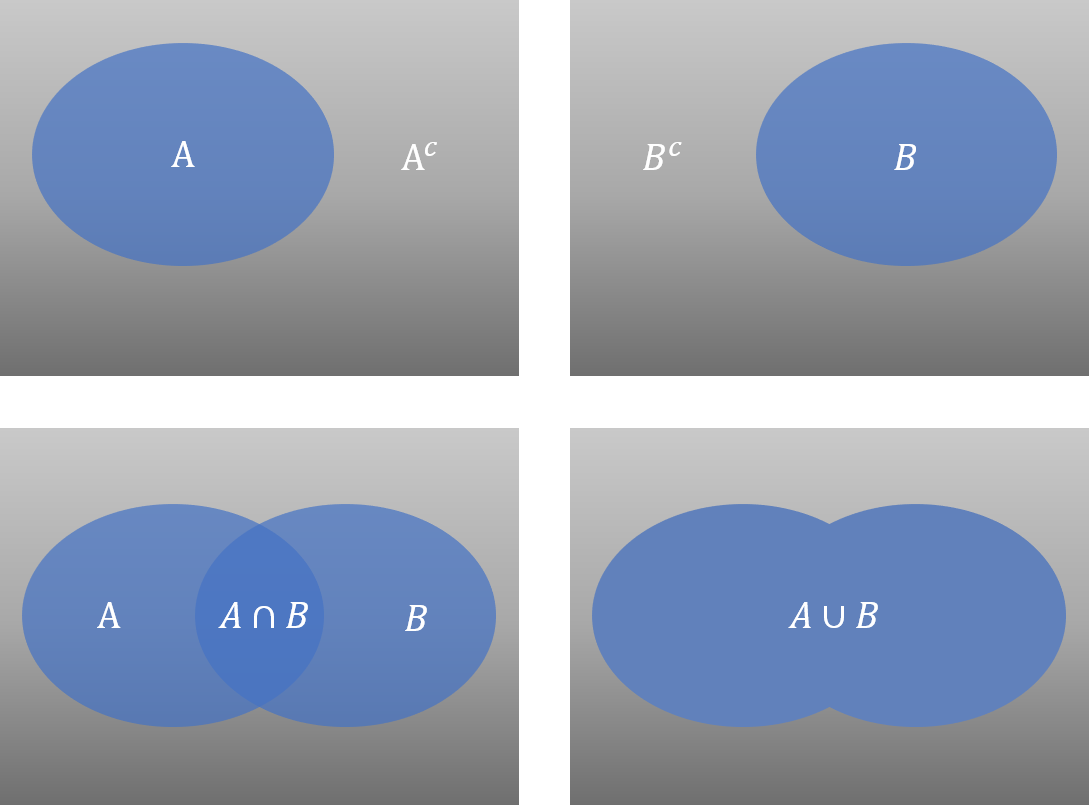
\includegraphics[width=1.0\linewidth]{boolean_algebra.png}
\end{figure}

举个简单的例子,如果$A$表示会打乒乓球的人,$B$表示会打篮球的人;则$A\cap B$表示既会打乒乓球又(AND)会打篮球的人;$A\cup B$表示所有会打乒乓球或者(OR)会打篮球的人;$A^c$表示所有所有不(NOT)会打乒乓球的人。

正如上面例中介绍到的,逻辑连接词$AND$、$OR$和$NOT$描述了由交集、并集和补集操作引起的集合的解释,表明\emph{集合操作(Set Operations)}和\emph{逻辑操作(Logic Operations)}之间存在密切的联系。

当我们能够将代数语句转化为逻辑语句后,我们就可以很容易地定义表示相同逻辑的不同代数。也就是用一个含有一系列用逻辑函数($AND,OR,NOT$)联系起来的变量($a,b,c,\dots$)的数学函数来表示一个或真或假的\emph{逻辑命题(Logical Proposition)}。
表\ref{tb:de_morgan_law}列出了部分所谓的\emph{De-Morgan定律(De-Morgan's Laws)},它给出了基本逻辑命题的句法等效版本。通过使用这些定律,我们可以从$\wedge$的所有实例或$\vee$的所有实例的任何逻辑表达式中系统地消除。这意味着我们可以将非常复杂的逻辑命题简化为形成两种标准形式之一,即连词的分离(即\emph{析取范式,Disjunctive Normal Form})或析取连词(即\emph{连词范式,Conjunctive Normal Form})。

因此,如果我们可以创建一些非常简单的基本门的硬件实现,例如,$NOT$, $AND$和$OR$,我们原则上可以将这些操作组合成非常复杂的电路。在经典的数字电路研究中包括许多这样的模块,比如加法器\cite[]{Mukherjee_Dhar_2014}、乘法器\cite[]{Shu_Haruo_2016}、滤波器\cite[]{Kumar_Agarwal_2021}等等,具体的相关内容将在后续章节进行介绍。

传统上,\emph{逻辑门(Logic Gate, LG)}被认为是一种接受一个或多个布尔值(即$FALSE$或$TRUE$)作为输入,并返回一个布尔值作为输出的物理设备。布尔值($FALSE$和$TRUE$)通常分别与位值$0$和$1$同义使用。逻辑门是现代计算机的关键部件。任何经典计算都可以分解成一系列逻辑门,每次只作用于几个比特。因此,逻辑门是所有现代计算机的核心。整体上各类基本的门电路可以分为两类:\emph{可逆门(Reversible Gate)}和\emph{不可逆门(Irreversible Gate)}。下面两小节将分别介绍他们。

\begin{table}
    \centering
    \caption[De-Morgan定律]{逻辑上等价的命题。这里通过使用\emph{De-Morgan定律},任何命题都可以单独使用$NOT$和$AND$表示,或者单独使用$NOT$和$OR$}
    \label{tb:de_morgan_law}
    \begin{tabular}[\linewidth]{L{8cm}L{4cm}}
        \toprule
        % % \rule{width}{height}
        % \rule{0pt}{1cm} %改变行高
        % \renewcommand\arraystretch{2}  % 2表示2倍行高,个人经验1.2比较好
        \textbf{逻辑等效形式} & \\
        \toprule 
        $a\wedge0=0$ & 0与\\
        $a\wedge1=a$ & 1与\\
        $a\vee 0=1$ & 0或\\
        $a\vee 1=a$ & 1或\\
        \midrule 
        $a\wedge a=a$ & 独立性\\
        $a\vee a=a$ & 独立性\\
        $a\wedge \neg a=0$ & 矛盾定理\\
        $a\vee \neg a=1$ & 无谓重复\\
        $ \neg \neg a=1$ & 双重否定\\
        \midrule 
        $a\vee b=b\vee a$ & 与的交换律\\
        $a\wedge b=b\wedge a$ & 或的交换律\\
        $a\vee (b\vee c)=(a\vee b)\vee c$ & 与的结合律\\
        $a\wedge (b\wedge c)=(a\wedge b)\wedge c$ & 或的结合律\\
        $a\wedge (b\vee c)=(a\wedge b)\vee (a\wedge c)$ & 分配律\\
        $a\vee (b\wedge c)=(a\vee b)\wedge (a\vee c)$ & 分配律\\
        \midrule
        $a\wedge (a\vee b)=a$ & 吸收律\\
        $a\vee (a\vee b)=a$ & 吸收律\\
        $a\wedge (\neg a\vee b)=a\vee b$ & 吸收律\\
        $a\vee (\neg a\vee b)=a\wedge b$ & 吸收律\\
        \midrule
        $\neg(a\wedge b)=(\neg a)\vee (\neg b)$ & De-Morgan定律\\
        $\neg(a\vee b)=(\neg a)\wedge (\neg b)$ & De-Morgan定律\\
        $(a\wedge b)\vee(a\wedge \neg b)=a$ & \\
        $a\Longrightarrow b=\neg a \vee b$ & \\
        $a\Longrightarrow b=\neg (a \vee \neg b)$ & \\
        \bottomrule
    \end{tabular}
\end{table}





\subsubsection[不可逆门:AND、OR、XOR]{不可逆门:AND、OR、XOR}

\begin{figure}
    \centering
    \caption[不可逻辑逆门]{不可逻辑逆门}
    \label{fig:irreversible_gates}
    \subcaptionbox{$AND$门图标\label{fig:and_gate}}{
        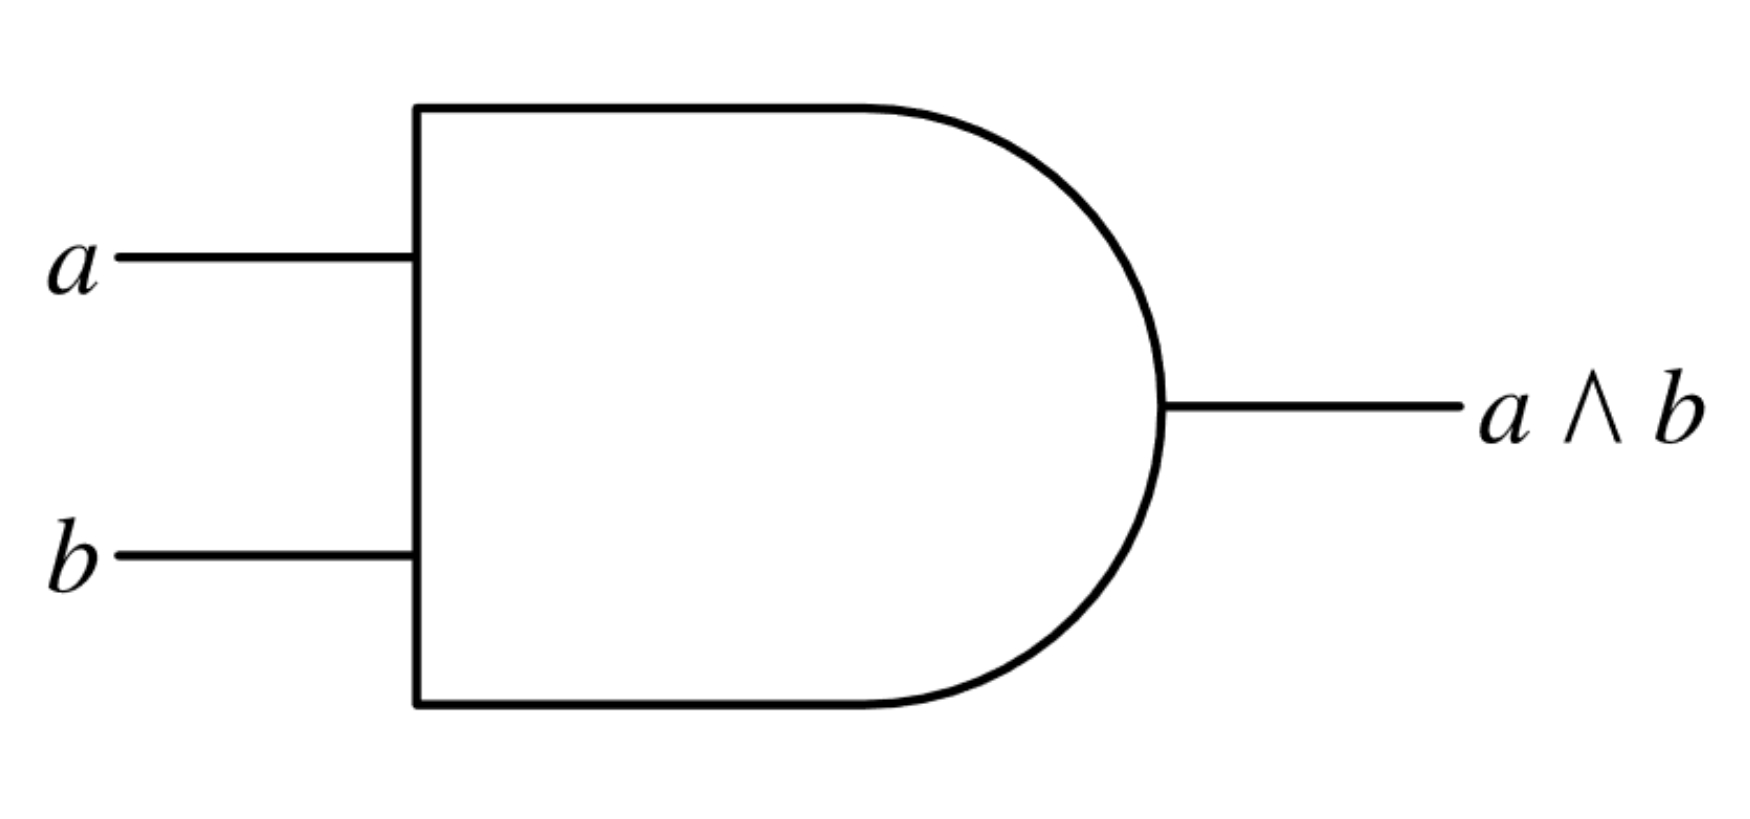
\includegraphics[width=0.3\linewidth]{and_gate.png}
    }
    \subcaptionbox{$OR$门图标\label{fig:or_gate}}{
        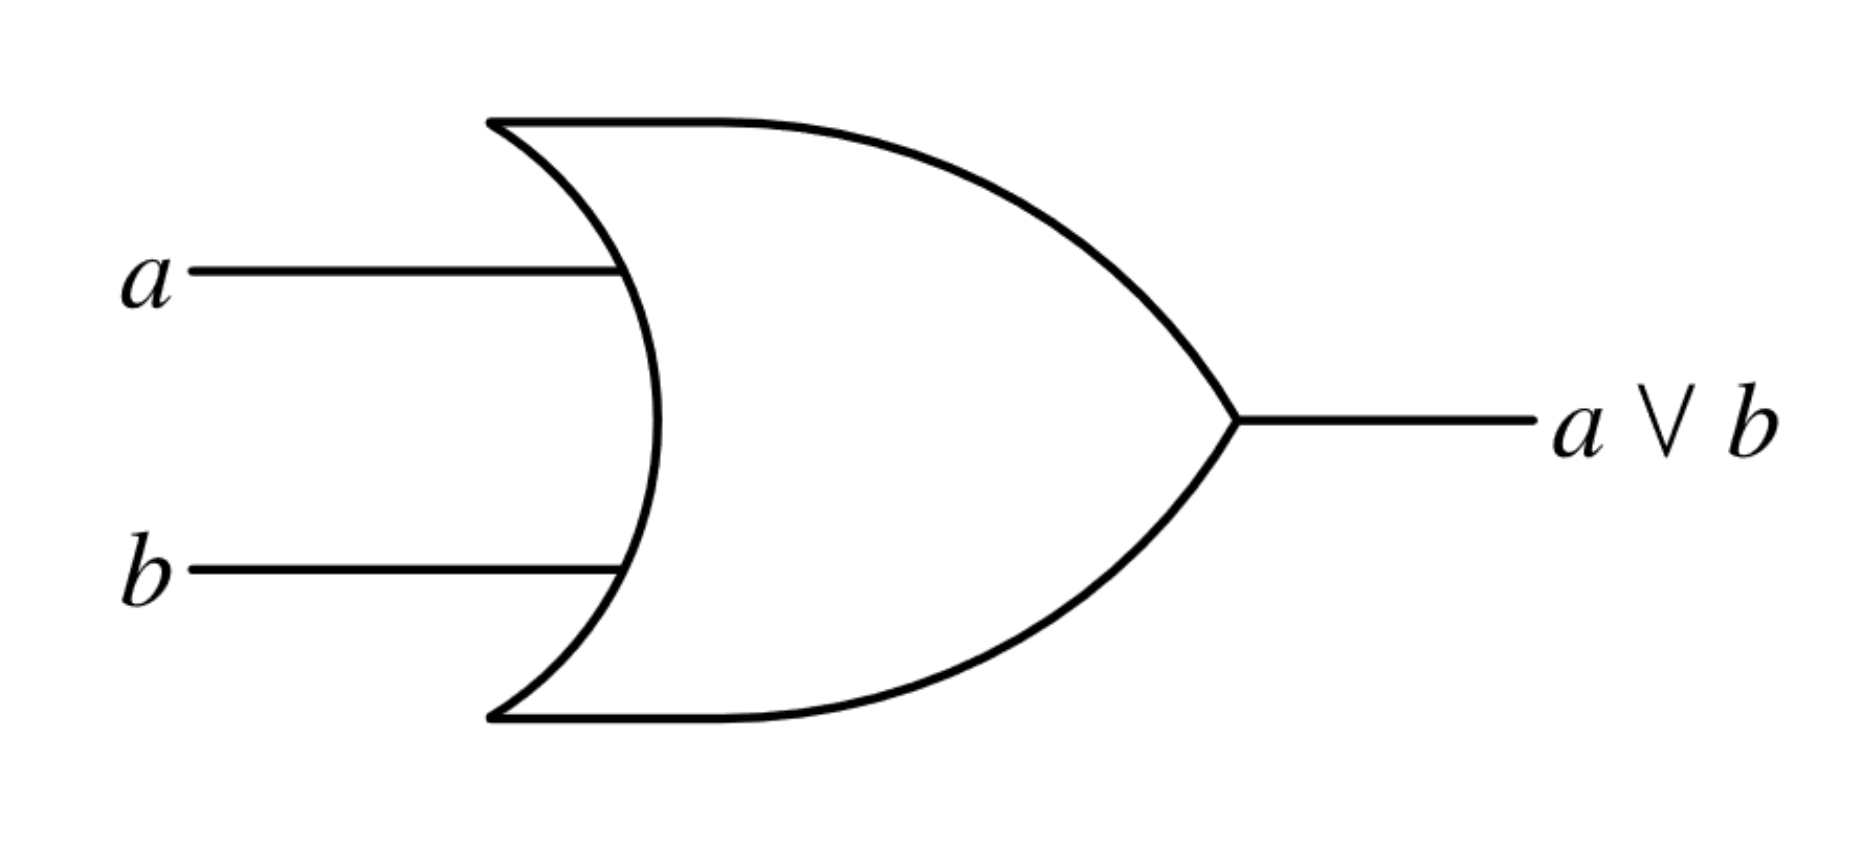
\includegraphics[width=0.3\linewidth]{or_gate.png}
    }
    \subcaptionbox{$XOR$门图标\label{fig:xor_gate}}{
        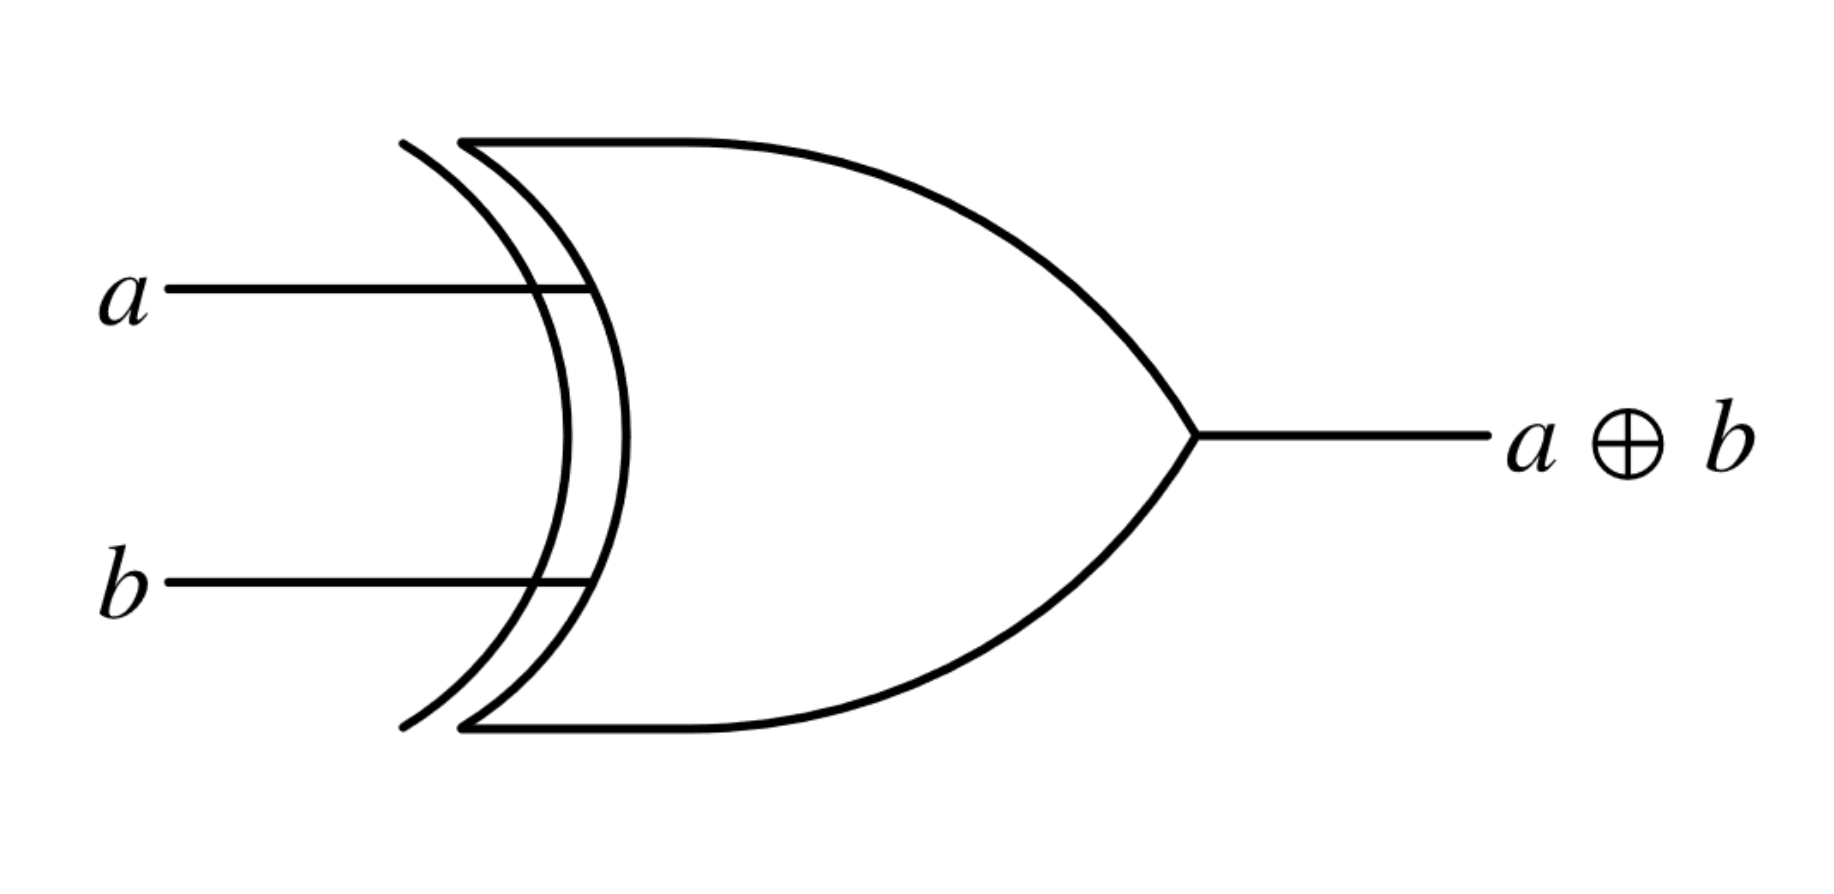
\includegraphics[width=0.3\linewidth]{xor_gate.png}
    }
\end{figure}

\begin{table}
    \centering
    \caption[不可逻辑逆门]{不可逻辑逆门}
    \subcaptionbox{$AND$门真值表\label{tb:and_gate}}{
        \begin{tabular}{C{1cm}C{1cm}C{1cm}}
            \toprule 
            \multicolumn{3}{c}{\textbf{AND}}\\
            \toprule
            a & b & $a\wedge b$ \\
            \hline
            0 & 0 & 0\\
            0 & 1 & 0\\
            1 & 0 & 0\\
            1 & 1 & 1\\
            \bottomrule
        \end{tabular}
    }
    \subcaptionbox{$OR$门的真值表\label{tb:or_gate}}{
        \begin{tabular}{C{1cm}C{1cm}C{1cm}}
            \toprule 
            \multicolumn{3}{c}{\textbf{OR}}\\
            \toprule
            a & b & $a\vee b$ \\
            \hline
            0 & 0 & 0\\
            0 & 1 & 1\\
            1 & 0 & 1\\
            1 & 1 & 1\\
            \bottomrule
        \end{tabular}
    }
    \subcaptionbox{$XOR$门的真值表\label{tb:xor_gate}}{
        \begin{tabular}{C{1cm}C{1cm}C{1cm}}
            \toprule 
            \multicolumn{3}{c}{\textbf{XOR}}\\
            \toprule
            a & b & $a\bigoplus b$ \\
            \hline
            0 & 0 & 0\\
            0 & 1 & 1\\
            1 & 0 & 1\\
            1 & 1 & 0\\
            \bottomrule
        \end{tabular}
    }
    
\end{table}


描述逻辑门动作的最好方法是用它的\emph{真值表(Truth Table)}。在真值表中,我们写下输入的所有可能的逻辑值及其相应的输出。例如,$AND$门的真值表如表\ref{tb:and_gate}所示。$AND$门在电路图中对应的图标如图\ref{fig:and_gate}所示。$AND$门在逻辑上是不可逆的,属于\emph{不可逆逻辑门(Irreversible Logic Gate, ILG)},这意味着我们无法为所有输出确定唯一的输入。具体来说,如果输出为$0$(即$FALSE$),则无法判断输入值是$00$、$01$还是$10$。换句话说,当$AND$门的输出为$0$时,它就会“擦除”一些信息。

同理,$OR$门的真值表如表\ref{tb:or_gate}所示。$OR$门对应的电路图标如图\ref{fig:or_gate}所示。$OR$门在逻辑上也是不可逆的,因为当它的输出为$1$(即$TRUE$)时,不可能说输入是$01$、$10$还是$11$。也就是说,当输出为$1$时,$OR$门再次擦除一些信息。

$OR$门有一种很常见变体,称为\emph{异或门(Exclusive-OR Gate)}(通常写为$XOR$或$\bigoplus$),事实证明它非常有用(因为很容易用晶体管实现)。$XOR$与$OR$相似,不同之处在于当两个输入都为$1$(即$TRUE$)时,它返回$0$(即$FALSE$)。$XOR$的真值表如表\ref{tb:xor_gate}所示。相应的异或电路图标如图\ref{fig:xor_gate}所示。




\subsubsection[可逆逻辑门:NOT、SWAP、CNOT]{可逆逻辑门:NOT、SWAP、CNOT}

上节介绍到的如$AND$门、$OR$门、$XOR$门等不可逆门在实践中应用十分广泛。随着数字芯片技术的不断发展,由于集成化的散热问题,不可逆门天然存在的限制逐渐被人们关注。基础物理理论告诉我们当信息被擦除时,一定伴随着能量的耗散\cite[]{Kastner_Schlatter_2023}。具体来说,每一比特信息的擦除会释放的能量为$kT\ln 2$,其中$k$是玻尔兹曼常数($k=1.3805\times 10^{-23}JK^{-1}$)而$T$是以\emph{凯尔文(Kelvin)}为单位的绝对温度。因此,即使所有其它能量损失机制从电路中消除了,由于信息擦除时发生的不可避免的能量损失,电路在操作时仍然会耗散能量。尽管当今在逻辑电路中由于逻辑不可逆性而导致的这种能量耗散与其它机制导致的能量耗散相比还比较小。然而,随着其它机制导致的能量耗散不断被克服,这种不可避免的信息擦除能量耗散将成为重要贡献,这将会阻碍计算芯片的进一步小型化和集成化。

克服上述问题的其中一个解决方案是修改现有的逻辑门使其仅使用\emph{可逆逻辑门(Reversible Logic Gate, RLG)}实现。在可逆逻辑门中,一个输入对应着一个确定的输出,反之亦然。因此,可逆门在起作用时永远不会删除任何信息,因此,可以向前运行基于可逆逻辑的计算以获得答案、复制的答案以及整个计算,然后再反向执行整个过程以恢复除用于复制中间点答案的小部分能量之外的所有能量。

可逆逻辑门的最简单例子是$NOT$门。$NOT$是一个\emph{1-input/1-output}门,它简单地反转它所处理的位值。$NOT$门的真值表如表\ref{tb:not_gate}所示。$NOT$门的电路图标如图\ref{fig:not_gate}所示。如果一个人知道输出位值,就可以明确地推断输入位值,反之亦然。

量子计算中非常重要的可逆门是\emph{受控非门($CNOT$)}。$CNOT$的真值表如表\ref{tb:cnot_gate}所示。$CNOT$门的电路图标如图2.9所示。$CNOT$门的效果是当且仅当第一个位设置为$1$时翻转第二个位的位值。也就是说,否定或不否定第二个位的决定由第一个位的值控制。这也是叫它受控非门的原因。
\begin{figure}
    \centering
    \caption{$NOT$门图标\label{fig:not_gate}}
    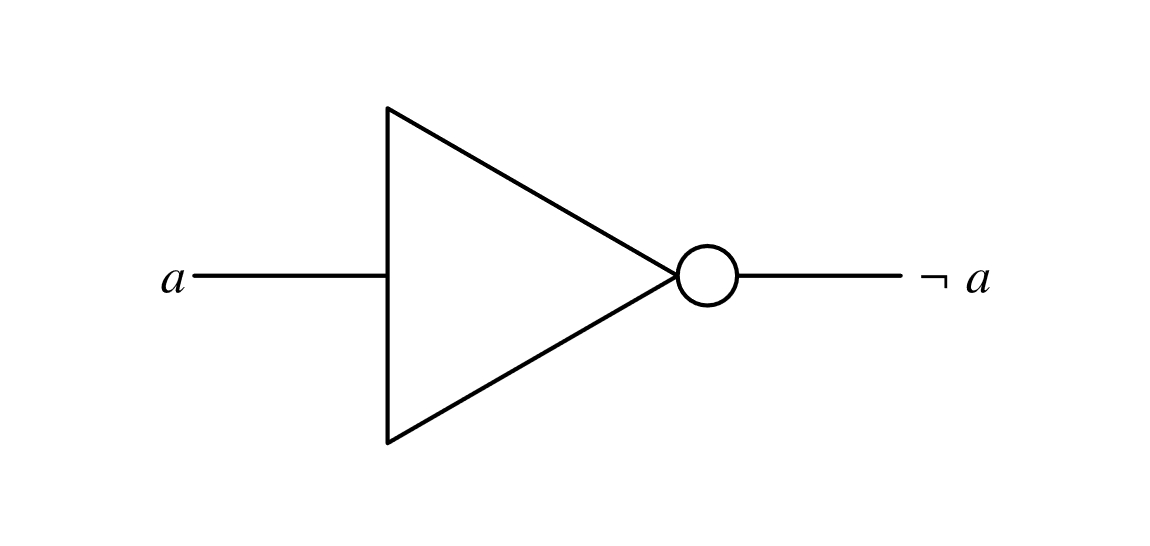
\includegraphics[width=0.8\linewidth]{not_gate.png}
\end{figure}

\begin{table}
    \centering
    \caption[\emph{NOT}门]{\emph{NOT}门\label{tb:not_gate}}
    \begin{tabular}{C{1.5cm}C{1.5cm}}
        \toprule 
        \multicolumn{2}{c}{\textbf{NOT}}\\
        \toprule
        a & $\neg a$  \\
        \hline
        0 & 1 \\
        1 & 0 \\
        \bottomrule
    \end{tabular}
\end{table}


\begin{figure}
    \centering
    \caption{$CNOT$门图标\label{fig:cnot_gate}}
    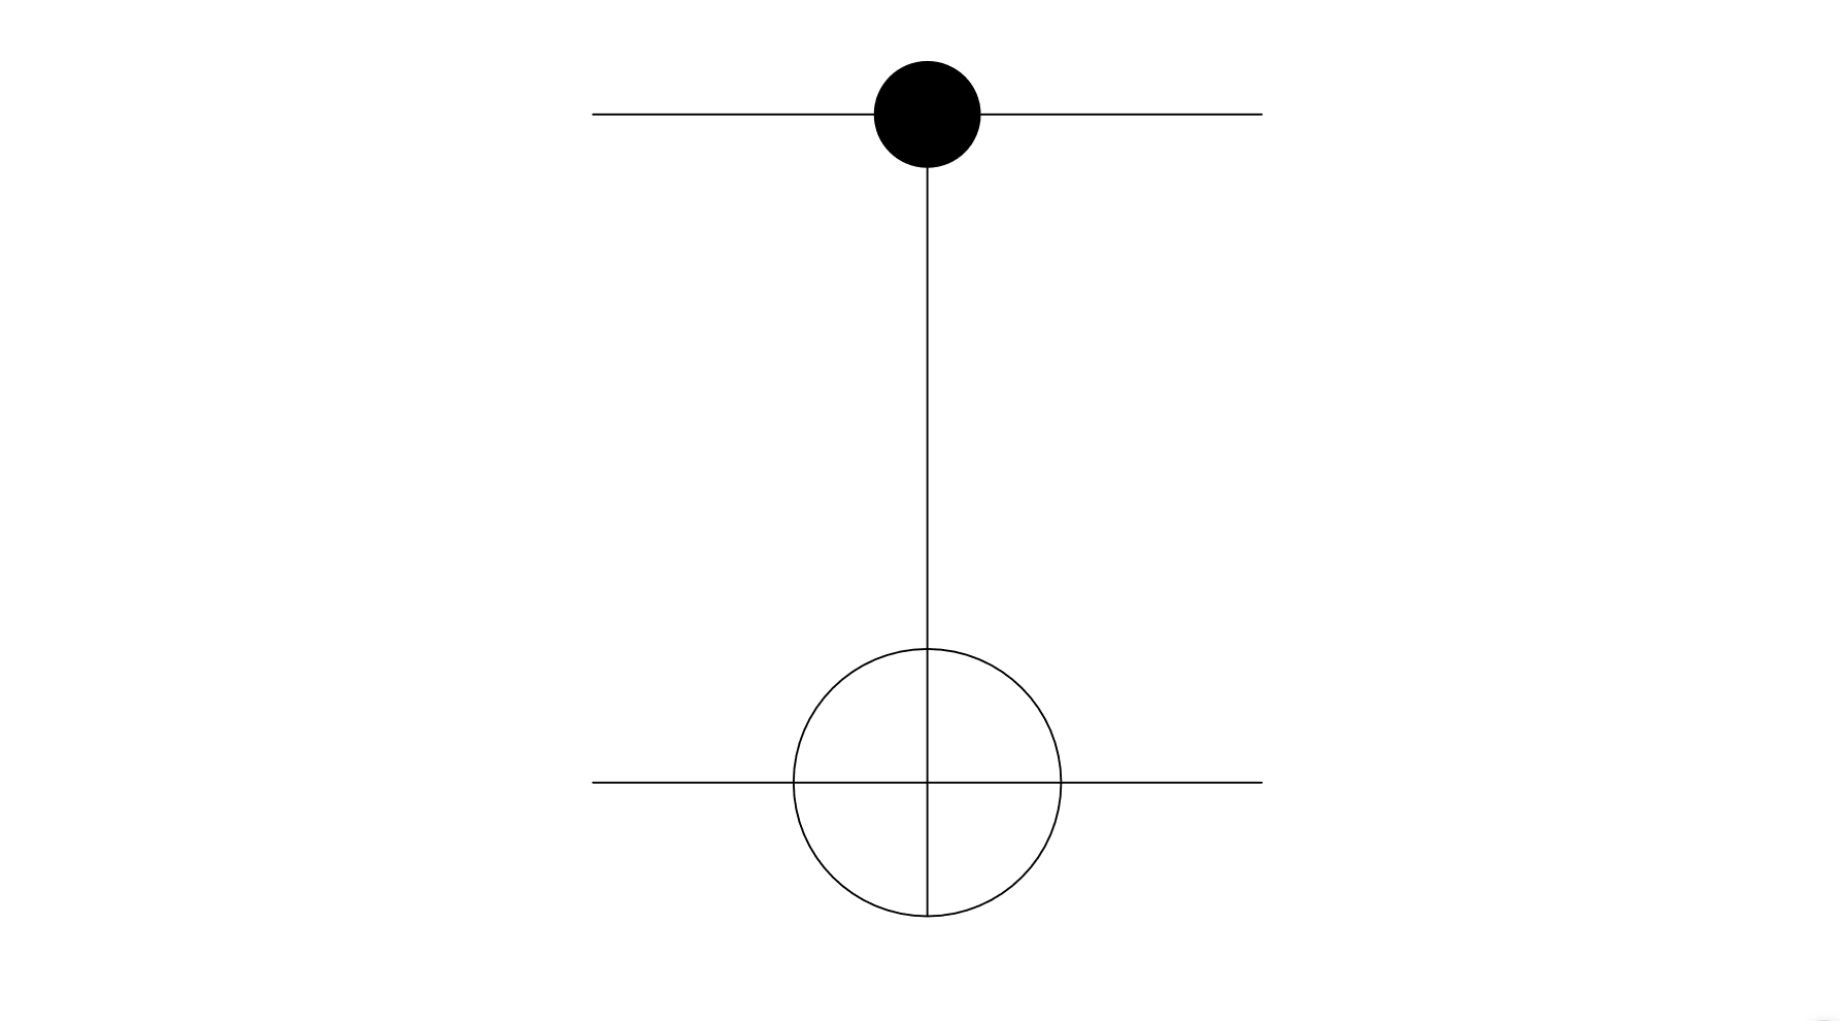
\includegraphics[width=0.8\linewidth]{cnot_gate.png}
\end{figure}

\begin{table}
    \centering
    \caption[\emph{CNOT}门]{\emph{CNOT}门\label{tb:cnot_gate}}
    \begin{tabular}{C{1cm}C{1cm}C{1cm}C{1cm}}
        \toprule 
        \multicolumn{4}{c}{\textbf{CNOT}}\\
        \toprule
        a & b & $a'$ & $b'$  \\
        \hline
        0 & 0 & 0 & 0 \\
        0 & 1 & 1 & 0 \\
        1 & 0 & 0 & 1 \\
        1 & 1 & 1 & 1 \\
        \bottomrule
    \end{tabular}
\end{table}
% \begin{figure}
%     \centering
%     \caption[可逆逻辑门]{可逆逻辑门}
%     \label{fig:reversible_gates}
%     \subcaptionbox{$NOT$门图标\label{fig:not_gate}}{
%         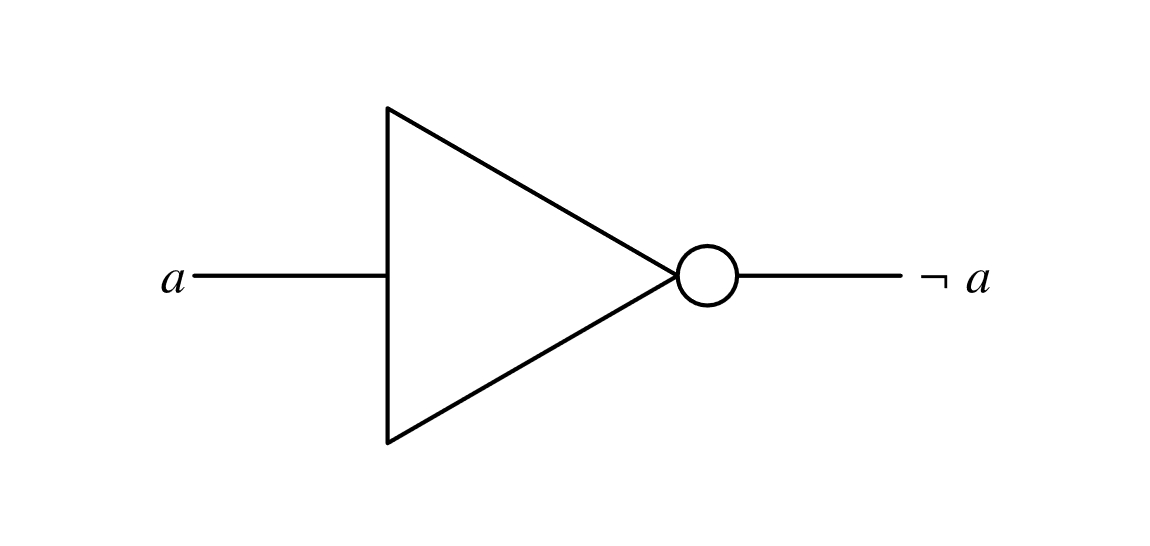
\includegraphics[width=0.45\linewidth]{not_gate.png}
%     }
%     \subcaptionbox{$CNOT$门图标\label{fig:cnot_gate}}{
%         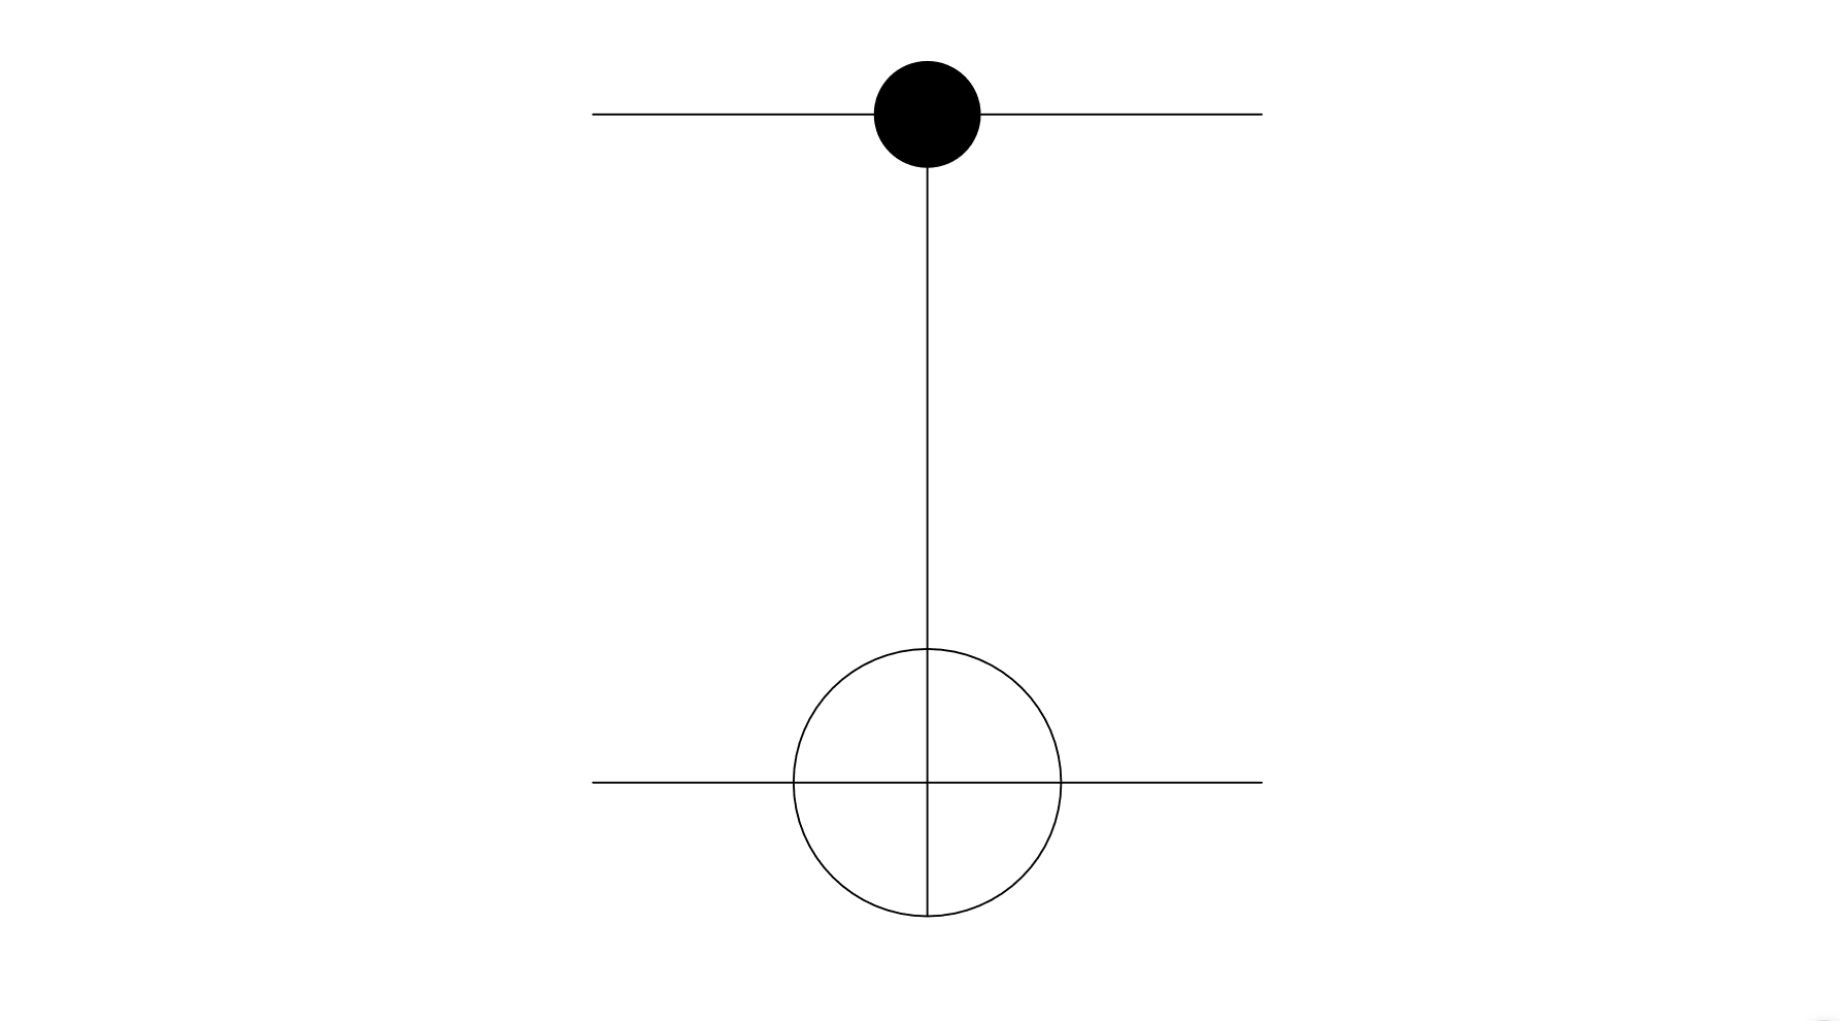
\includegraphics[width=0.45\linewidth]{cnot_gate.png}
%     }
% \end{figure}

% \begin{table}
%     \centering
%     \caption[可逆逻辑门]{可逆逻辑门}
%     \subcaptionbox{\emph{NOT}门\label{tb:not_gate}}{
%         \begin{tabular}{C{1.5cm}C{1.5cm}}
%             \toprule 
%             \multicolumn{2}{c}{\textbf{NOT}}\\
%             \toprule
%             a & $\neg a$  \\
%             \hline
%             0 & 1 \\
%             1 & 0 \\
%             \bottomrule
%         \end{tabular}
%     }
%     \subcaptionbox{\emph{CNOT}门\label{tb:cnot_gate}}{
%         \begin{tabular}{C{1cm}C{1cm}C{1cm}C{1cm}}
%             \toprule 
%             \multicolumn{4}{c}{\textbf{CNOT}}\\
%             \toprule
%             a & b & $a'$ & $b'$  \\
%             \hline
%             0 & 0 & 0 & 0 \\
%             0 & 1 & 1 & 0 \\
%             1 & 0 & 0 & 1 \\
%             1 & 1 & 1 & 1 \\
%             \bottomrule
%         \end{tabular}
%     }
% \end{table}




注意$CNOT$门不仅是一种RLG,还是一种\emph{通用逻辑门(Universal Logic Gate, ULG)}。也就是说以它为基础可以实现任何其它类型的门,比如$AND$、$OR$等等,进一步地可以只用$CNOT$搭建网络实现任何计算。ULG除了$CNOT$门外,还有$TOFFOLI$门\cite[]{Maslov_Dueck_Miller_2005}、$FREDKIN$门\cite[]{Adamatzky_2017}等等。$TOFFOLI$门和$FREDKIN$门都属于RLG,比如$TOFFOLI$门的真值表如表\ref{tb:toffoli_gate}所示,它的图标如图\ref{fig:toffoli_gate}所示。
\begin{table}
    \centering
    \caption[TOFFOLI]{\emph{TOFFOLI}门真值表}
    \label{tb:toffoli_gate}
    \begin{tabular}{C{1cm}C{1cm}C{1cm}C{1cm}C{1cm}C{1cm}}
        \toprule
        a & b & c & $a'$ & $b'$ & $c'$\\
        \toprule 
        0 & 0 & 0 & 0 & 0 & 0\\
        0 & 0 & 1 & 0 & 0 & 1\\
        0 & 1 & 0 & 0 & 1 & 0\\
        0 & 1 & 1 & 0 & 1 & 1\\
        1 & 0 & 0 & 1 & 0 & 0\\
        1 & 0 & 1 & 1 & 0 & 1\\
        1 & 1 & 0 & 1 & 1 & 1\\
        1 & 1 & 1 & 1 & 1 & 0\\
        \bottomrule
    \end{tabular}
\end{table}
\begin{figure}
    \centering
    \caption[\emph{TOFFOLI}门图标]{\emph{TOFFOLI}门图标}
    \label{fig:toffoli_gate}
    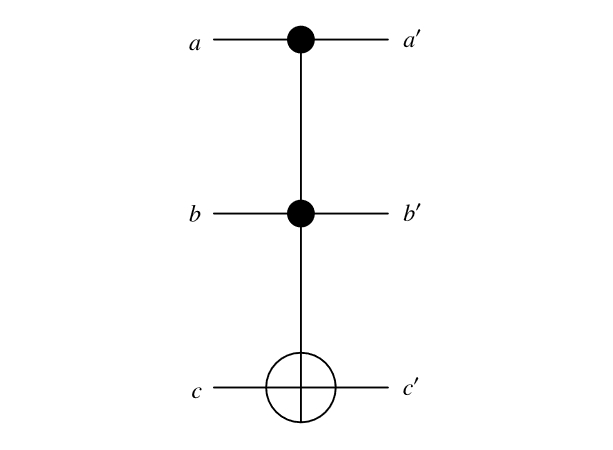
\includegraphics[width=0.8\linewidth]{toffoli_gate.png}
\end{figure}

\subsection[量子逻辑门]{量子逻辑门}
前面我们已经讨论过经典的不可逆和经典的可逆门,这使我们能够更好地理解量子门的优越性。就像任何经典计算都可以分解成一系列经典逻辑门,这些门一次只作用于几个经典比特,因此任何量子计算也可以分解成一系列量子逻辑门,这些门一次只作用于几个量子比特。主要区别在于,虽然经典逻辑门操纵经典位值$0$或$1$,但量子门可以操纵任意多量子态,包括计算基态的任意叠加,这些量子态也经常纠缠在一起。因此,量子计算的逻辑门比经典计算的逻辑门更加多样化。

通常我们使用\emph{泡利矩阵(Pauli Matrices)},$\mathbb{1}, \mathbfit{X}, \mathbfit{Y}, \mathbfit{Z}$,来描述单量子比特。单量子比特既是厄米特(Hermitian)的也是幺正(Unitary)的,任何1-量子比特哈密顿量总是可以写成泡利矩阵的加权和:
\begin{align}
    \mathbb{1}=\begin{pmatrix}
        1 & 0 \\
        0 & 1 \\
    \end{pmatrix}, \quad \mathbfit{X}=\begin{pmatrix}
        0 & 1 \\
        1 & 0 \\
    \end{pmatrix}, \quad  \mathbfit{Y}=\begin{pmatrix}
        0 & -i \\
        i & 0 \\
    \end{pmatrix}, \quad  \mathbfit{Z}=\begin{pmatrix}
        1 & 0 \\
        0 & -1 \\
    \end{pmatrix}
\end{align}

实际上泡利矩阵$\mathbfit{X}$和经典逻辑门中的$NOT$门对应,有:
\begin{align}
    \mathbfit{X}\equiv NOT = \begin{pmatrix}
        0 & 1 \\
        1 & 0 \\
    \end{pmatrix}
\end{align}

也就是说$\mathbfit{X}$可以类似经典比特的$NOT$门用来翻转量子比特的状态,即:
\begin{align}
    \mathbfit{X}\ket{0}=\begin{pmatrix}
        0 & 1 \\
        1 & 0 \\
    \end{pmatrix}\cdot \begin{pmatrix}
         1 \\
         0 \\
    \end{pmatrix}=\begin{pmatrix}
        0 \\
        1 \\
   \end{pmatrix}=\ket{1}\\
   \mathbfit{X}\ket{1}=\begin{pmatrix}
    0 & 1 \\
    1 & 0 \\
\end{pmatrix}\cdot \begin{pmatrix}
     0 \\
     1 \\
\end{pmatrix}=\begin{pmatrix}
    1 \\
    0 \\
\end{pmatrix}=\ket{0}\\
\end{align}

但是注意$\mathbfit{X}$并不是一个真正意义上的\emph{量子非门(Quantum Not Gate, QNG)},实际上并不存在一个通用的QNG。

有一个很重要的量子门值得在这里被介绍,它就是\emph{Hadamard门(Hadamard Gate)},它的定义如下\cite[]{PRUDÊNCIO_2013}:
\begin{align}
    \mathbfit{H}=\frac{1}{\sqrt{2}}\begin{pmatrix}
        1 & 1 \\
        1 & -1 \\
    \end{pmatrix}
\end{align}

它的最广泛的应用是用来制备量子叠加态,基本的过程示意如下:
\begin{align}
    \mathbfit{H}\ket{0}=\frac{1}{\sqrt{2}}\begin{pmatrix}
        \ket{0}+\ket{1}
    \end{pmatrix}\\
    \mathbfit{H}\ket{1}=\frac{1}{\sqrt{2}}\begin{pmatrix}
        \ket{0}-\ket{1}
    \end{pmatrix}\\
\end{align}

这是一个看似简单的看门,但它有一个重要的性质。进一步地,它可以制备$n$个比特的叠加态,这些态将会均匀地分布在$[0, 1, ..., 2^n-1]$的范围上:
\begin{align}
    \mathbfit{H}\ket{0}\otimes\mathbfit{H}\ket{0}\otimes\dots\otimes\mathbfit{H}\ket{0}=\frac{1}{\sqrt{2^n}}\sum_{j=0}^{2^n-1}\ket{j}
\end{align}

其中$\ket{j}$是是由二进制数索引的计算基态,该二进制数将对应于 十进制符号中的数字$j$。比如对于$3$量子比特的寄存器来说,$\ket{0}$表示计算基态$\ket{000}$;$\ket{1}$表示计算基态$\ket{001}$;··· ;$\ket{7}$表示计算基态$\ket{111}$。

这些本征态意味着可以使用$n$比特同时写入的所有可能比特串组合。它实际上是量子计算最重要的技巧之一,因为它实现了仅使用多项式多次操作而将指数多的索引加载到量子计算机中。如果自然界没有种方法,我们则必须像我们在经典计算中所做的那样一个一个单独输入不同的位串,那么量子计算在计算复杂性方面取得突破的可能性要小得多。

在量子门的阐述中有一个门是绝对不能忽略的,那就是量子$CNOT$门。和经典$CNOT$门一样,它会根据一个比特的状态来决定是否翻转两一个比特的状态,比如:
\begin{align}
    \ket{00}\overset{CNOT}{\longrightarrow}\ket{00}\\
    \ket{01}\overset{CNOT}{\longrightarrow}\ket{01}\\
    \ket{10}\overset{CNOT}{\longrightarrow}\ket{11}\\
    \ket{11}\overset{CNOT}{\longrightarrow}\ket{10}\\
\end{align}

其中第二个比特(靠右的)的状态受到第一个比特(靠左的)的状态控制。由于$CNOT$门是一个通用的门,因此只要一个量子物理体系能够实现$CNOT$门,那么这个体系就具备了实现通用量子计算机的前景\cite[]{Zajac_Sigillito_Russ_Borjans_Taylor_Burkard_Petta_2018,Zhu_Cheng_Zhu_Chen_Guan_2022}。


\subsection[量子算法]{量子算法}









\section[量子计算的不同实现平台]{量子计算的不同实现平台}
\textcolor{red}{这部分需要分别找各个平台的文献进行整理,每个平台找一到两篇吧}
\subsection[离子量子计算]{离子量子计算}

\subsection[超导量子计算]{超导量子计算}

\subsection[原子量子计算]{原子量子计算}

\subsection[硅基量子计算]{硅基量子计算}

\subsection[光量子计算]{光量子计算}

\subsection[拓扑量子计算]{拓扑量子计算}







% !TeX root = ../sustechthesis-example.tex

\chapter[离子阱量子计算系统]{离子阱量子计算系统\label{section:ion_trap_quantum_computation_system}}

% \textcolor{red}{
% 这部分简单讲一下离子阱量子计算的发展历史,重点介绍离子阱量子计算系统的基本组成,不针对特别具体的系统...
% }

% \section[离子阱的发展]{离子阱的发展}

% \textcolor{red}{这部分主要参考文献\cite[p2]{Bruzewicz_Chiaverini_McConnell_Sage_2019}}




% \section[离子阱的囚禁]{离子阱的囚禁}

\section[离子在RF阱中的经典运动]{离子在RF阱中的经典运动\label{section:ion_classical_motion}}
% \textcolor{red}{主要参考文献\cite[chap2-A]{Leibfried_Blatt_Monroe_Wineland_2003}}

离子阱采用射频阱对离子进行动态囚禁,最具代表性的一类是四极阱,它及它的一些变型也是目前在离子阱量子计算研究中应用最广泛的一类离子阱。四极阱的电势描述如下:
\begin{align}
    % \label{eq:quadrupolar_trap_potential}
    \Phi(x, y, z, t) = &U\frac{1}{2}(\alpha x^2 + \beta y^2 + \gamma z^2) \label{eq:time_independent_part}\\
    \label{eq:time_dependent_part}
    &+ \tilde{U}\cos (\omega_{rf}t)\frac{1}{2}(\alpha ' x^2 + \beta ' y^2 + \gamma ' z^2) 
\end{align}
其中$\Phi(x, y, z, t)$是四极阱的电势,公式\eqref{eq:time_independent_part}是不依赖时间的项,公式\eqref{eq:time_dependent_part}是随时间变化的项。整个电势的表达式每时每刻都要满足拉普拉斯方程(Laplace equation)$\Delta \Phi=0$的约束条件,从中可以导出整个四极阱的几何参数约束:
\begin{align}
    \alpha + \beta + \gamma =0,\\
    \alpha ' + \beta ' + \gamma ' =0
\end{align}

其中各参数的定义在公式\eqref{eq:time_independent_part}和公式\eqref{eq:time_dependent_part}定义。从这些限制可以明显看出,在自由空间中电势不可能稳定地产生局部三维最小值,因此电势只可能以动态方式来对离子进行囚禁。幸运的是,通过对四极阱几何参数的选择,再结合适当的驱动微波的频率和驱动电压我们可以做到这一点。其中一种几何参数选择如下:
\begin{align}
    -(\alpha + \beta )= \gamma > 0,\\
    \alpha ' = - \beta '
\end{align}
这种几何参数的设置会使离子在$x,y$平面上动态地被囚禁,在$z$方向上静态地被囚禁。在这种设置的离子阱中,多个离子会沿着$z$轴形成线性的离子链,这便是人们所知的\emph{线性离子阱(Linear Trap)},也被称为\emph{Paul Trap}\cite[]{Paul_1990}。在接下来的两小节里我将介绍囚禁离子的经典运动方程及其解析解(第\ref{section:classical_motion}节),并给出这些解的低阶近似(第\ref{section:lowest_order_approximation}节)。

\subsection[经典运动方程]{经典运动方程\label{section:classical_motion}}

一个质量为$m$电荷量为$Z|e|$的粒子在如公式\eqref{eq:time_independent_part}所描述的电场中的经典运动方程由Paul等人\cite[p415]{Paul1958}给出。粒子的运动在空间坐标方向上中是解耦的。下面只讨论$x$方向上的运动;其他方向可以类似地处理。运动方程如下:
\begin{align}
    \ddot{x}=-\frac{Z|e|}{m}\frac{\partial \Phi}{\partial x}=-\frac{Z|e|}{m}[U\alpha + \tilde{U}\cos(\omega_{rf}t)\alpha ']x
\end{align}

经过下面的参数代换,这个方程可以转化为标准的\emph{马修方程(Mathieu Equation, ME)}形式:
\begin{align}
    \frac{d^2x}{d\xi^2}+[a_x-2q_x\cos(2\xi)]x=0\label{eq:mathieu_equation}
\end{align}

相应的参数代换为:
\begin{align}
    \xi=\frac{\omega_{rf}t}{2},\ a_x=\frac{4Z|e|U\alpha}{m\omega_{rf}^2},\ q_x=\frac{2Z|e|\tilde{U}\alpha '}{m\omega_{rf}^2}\label{eq:parameters_substitution}
\end{align}

ME方程属于一般的周期系数微分方程。它的稳定解的一般形式可以由\emph{弗洛奎定理(Floquet Theorem)}导出\cite[]{McLachlan, McQuarrie}:
\begin{align}
    x(\xi)=&Ae^{i\beta_x\xi}\sum_{n=-\infty}^{\infty}C_{2n}e^{i2n\xi}\\
    &+ Be^{-i\beta_x\xi}\sum_{n=-\infty}^{\infty}C_{2n}e^{-i2n\xi}\label{eq:mathieu_solution}
\end{align}

其中实值特征指数$\beta_x$和系数$C_{2n}$仅是$a_x$和$q_x$的函数,不依赖于初始条件。$A$和$B$是任意常数,可用于满足边界条件或规格化特解。将公式\eqref{eq:mathieu_solution}代入公式\eqref{eq:mathieu_equation}可以得到一个递归关系:
\begin{align}
    C_{2n+2}-D_{2n}C_{2n}+C_{2n-2}=0,\\
    D_{2n}=[a_x-(2n+\beta_x)^2]/q_x\label{eq:recursion_raltion}
\end{align}

这一递归关系将实值特征指数$\beta_x$、系数$C_{2n}$与$a_x$、$q_x$联系起来。通过进一步地整理也可以得到$C_{2n}$的表达式:
\begin{align}
    C_{2n+2}=\frac{C_{2n}}{D_{2n}-\frac{1}{D_{2n+2}-\frac{1}{\dots}}}\\
    C_{2n}=\frac{C_{2n-2}}{D_{2n}-\frac{1}{D_{2n-2}-\frac{1}{\dots}}}\label{eq:c_2n_fraction}
\end{align}

利用结合上述公式$\beta_x$也可以计算:
\begin{align}
    \beta_x^2=a_x-q_x\left(\frac{1}{D_0-\frac{1}{D_2-\frac{1}{\dots}}} + \frac{1}{D_0-\frac{1}{D_{-2}-\frac{1}{\dots}}}\right) \label{eq:beta_x_fraction}
\end{align}

可以根据所需的精度,选择截断公式\eqref{eq:c_2n_fraction}和公式\eqref{eq:beta_x_fraction}中的连分式来获取相应的结果。
实际上,对于实验中常用到的典型$a_x$和$q_x$值,连分式中高阶项的贡献会迅速下降。

% \textcolor{red}{这里的$a_x, q_x$具体的含义后面有时间了可以再看看。}

\subsection[低阶近似]{低阶近似\label{section:lowest_order_approximation}}
实际实验系统中采用的在公式\eqref{eq:parameters_substitution}中定义的参数往往是满足$(|a_x|,q_x^2)\ll 1$的。在此条件下,假设$C_{\pm 4}\simeq 0$,则可以得到$x(t)$轨迹的\emph{低阶近似(Lowest-order Approximation)}。再同时设置初始条件$A=B$,公式\ref{eq:recursion_raltion}可以得到:
\begin{align}
    \beta_x\approx \sqrt{a_x+q_x^2/2},\\
    x(t)\approx2AC_0\cos\left(\beta_x\frac{\omega_{rf}}{2}t\right)\left[1-\frac{q_x}{2}\cos(\omega_{rf}t)\right]\label{eq:classical_motion_solution}
\end{align}

囚禁离子在$x$方向上的轨迹$x(t)$的由频率为$\nu=\beta_x\omega_{rf}/2\ll \omega_{rf}$的谐波振荡叠加频率为$\omega_{rf}$的RF频率造成的\emph{驱动位移}组成,分别称为\emph{长期运动(Secular-motion)}和\emph{微运动(Micro-motion)}两者相位相差$180^\circ$;
离子在离子阱中的微运动的频率为$\omega_{rf}\ll \nu$,且其振幅为长期运动振幅的$q_x/2\ll 1$,这也是它被称为微运动的原因。如果忽略微运动,则长期运动可以近似为频率为$\nu$的谐振子的运动。在大多数情况下,如果离子处于相当低的动能,即使我们用量子力学的方法来处理离子的质心运动,这个处理也是合理的。


\section[离子在RF阱中的量子力学运动]{离子在RF阱中的量子力学运动\label{section:quantum_motion}}
% \textcolor{red}{主要参考文献\cite[chap2-B]{Leibfried_Blatt_Monroe_Wineland_2003}}

如第\ref{section:ion_classical_motion}节中已经讨论过的,经典中的运动分析似乎已经可以很好地描述离子在离子阱中的运动了。但是,由于四极阱产生的囚禁势场不是静态的而是与时间相关的,因此不能理所当然地认为在有效时间平均势中量化运动已经为我们提供了囚禁离子足够的图景。实际上,在离子阱的实验中,即使是对离子陷阱中的冷却过程的简单解释,以及对非经典状态的描述,也都依赖于运动的量子力学图景的。

在接下来的两小节里,我将根据文献\cite[]{Arimondo_Phillips_Strumia_1992}中的方法导出囚禁离子在射频场中的量子力学表述。同时在这里讨论,在实验中使用的捕获参数范围内,囚禁离子的量子化运动可以用静态谐振子来近似。

\subsection[量子力学运动方程]{量子力学运动方程}
对于囚禁离子运动的量子力学处理,我们假设与时间相关的势在囚禁离子质心的三个笛卡尔坐标中的每一个中都是二次的(一维谐振子势\cite[]{Solimeno_Di_Porto_Crosignani})。然后,与经典运动一样,问题可分为三个一维问题。在一维中,用各自的算子$\hat{x}$替换坐标$x$,于是可以将与时间相关的势$V(T)$写为:
\begin{align}
    V(t)=\frac{m}{2}W(t)\hat{x}^2
\end{align}

其中,
\begin{align}
    W(t)=\frac{\omega_{rf}^2}{4}\left[a_x+2q_x\cos(\omega_{rf}t)\right]
\end{align}

可以被认为是一个时变弹簧常数,它的作用类似于在静态势谐振子中$\omega^2$的作用。在以上的定义下,囚禁离子运动的哈密顿量$H^{(m)}$的形式和我们在量子力学中处理的静态谐振子的哈密顿量很相似:
\begin{align}
    \hat{H}^{(m)}=\frac{\hat{p}^2}{2m}+\frac{m}{2}W(t)\hat{x}^2\label{eq:static_harmiltonian_oscillator}
\end{align}

于是我们可以很轻松地写出这些运动算子在\emph{海森堡图景(Heisenberg Picture)}下的的方程:
\begin{align}
    \dot{\hat{x}}= \frac{1}{i\hbar}\left[\hat{x,\hat{H}^{(m)}}=\frac{\hat{p}}{m}\right],\\
    \dot{\hat{p}}= \frac{1}{i\hbar}\left[\hat{p},\hat{H}^{(m)}\right]=-mW(t)\hat{x}
\end{align}

他们的一个更紧凑的方程形式如下:
\begin{align}
    \ddot{\hat{x}}+W(t)\hat{x}=0 \label{eq:quantum_motion_equation}
\end{align}

如果用函数$u(t)$替换算子$\hat{x}$,我们可以很容易验证这个公式\eqref{eq:quantum_motion_equation}与\emph{马修方程}\eqref{eq:mathieu_equation}是等价的。这就是我们能够借助前面所叙述的马修方程的解来寻找公式\eqref{eq:quantum_motion_equation}的解。添加边界条件:
\begin{align}
    u(0)=1,\ \hat{u}(0)=i\nu \label{eq:boundary_condition}
\end{align}

这对应于公式\eqref{eq:mathieu_solution}中的$A=1,\ B=0$,可以得到:
\begin{align}
    u(t)=e^{i\beta_x\omega_{rf}/2}\sum_{n=-\infty}^{\infty} C_{2n}e^{i n\omega_{rf}t}\equiv e^{i\beta_x\omega_{rf}t/2}\Phi(t) \label{eq:ut_expression}
\end{align}

其中$\Phi(t)$是一个周期为$T=2\pi/\omega_{rf}$的周期函数。于是公式\eqref{eq:boundary_condition}变为:
\begin{align}
    u(0)=\sum_{n=-\infty}^{\infty}C_{2n}=1,\ \nu = \omega_{rf}\sum_{n=-\infty}^{\infty}C_{2n}(\beta_x/2+n)
\end{align}

这个解及其复共轭是线性独立的;因此,它们服从\emph{Wronskian恒等式}:
\begin{align}
    u^*(t)\dot{u}(t)-u(t)\dot{u}^*(t)=u^*(0)\dot{u}(0)-u(0)\dot{u}^*(0)=2 i \mu
\end{align}

未知坐标$\hat{x}(t)$和$u(t)$满足相同的微分方程,因此复杂的线性组合:
\begin{align}
    \hat{C}(t)=\sqrt{\frac{m}{2\hbar \nu}}i\left\{u(t)\dot{\hat{x}(t)-\dot{u}(t)\hat{x}(t)}\right\} \label{eq:complex_combination}
\end{align}

与其如下的Wronskian恒等式成正比,并且在时间上也是恒定的:
\begin{align}
    \hat{C}(t)=\hat{C}(0)=\frac{1}{\sqrt{2m \hbar \nu}}\left[m\nu\hat{x}(0)+i\hat{p}(0)\right]
\end{align}

此外,等式右边恰好是质量$m$和频率$\nu$的在静态谐振子势场中的湮灭算符:
\begin{align}
    \hat{C}(t)=\hat{C}(0)=\hat{a}
\end{align}
也就是说有如下式:
\begin{align}
    \left[\hat{C},\hat{C}^\dagger\right]=\left[\hat{a},\hat{a}^\dagger=1\right]
\end{align}

这个静态势场中的谐振子在后续将被称为\emph{参考谐振子(Reference Oscillator)}。

海森堡算符$\hat{x}(t)$和$\hat{x}(t)$可以用$u(T)$和参考振荡器的算符用公式\eqref{eq:complex_combination}重新表示:

\begin{align}
    \hat{x}(t)=\sqrt{\frac{\hbar}{2m\nu}}\left\{\hat{a}u^*(t)+\hat{a}^\dagger u^(t)\right\},\\
    \hat{p}(t)=\sqrt{\frac{\hbar m}{2\nu}}\left\{\hat{a}\dot{u}^*(t)+\hat{a}^\dagger \dot{u}^(t)\right\}
\end{align}

所以囚禁离子的整个时间依赖性由特殊解$u(t)$及其复共轭给出。
这样一来,对于接下来的计算,在海森堡图景中表述一些列的时间依赖波函数就很方便了。同样,上面使用的参考振荡子也将非常有帮助。与静态势的情况类似,我们将考虑一系列的基态$\ket{n,t}$,其中$n=1,2,\dots,\infty$。这些状态被称为谐波振荡器\emph{数态(Fock States)}的动态对应物。参考振荡子$\ket{n=0}_\nu$的基态满足条件:
\begin{align}
    \hat{a}\ket{n=0}_\nu=\hat{C}(t)\ket{n=0}_\nu=0 \label{eq:obey_condition}
\end{align}

由于海森堡算子$\hat{C}$是通过$\hat{C}(t)=\hat{U}^\dagger(t)\hat{C}_S\hat{U}(t)$与$\hat{C}_S$联系起来的,我们可以很快得到(其中$\hat{U}(t)=\exp{\left[-(i/\hbar)\hat{H}^{(m)}\right]}$):
\begin{align}
    \hat{C}_S(t)\hat{U}(t)\ket{n=0}_\nu=\hat{C}_S(t)\ket{n=0,t}=0 \label{eq:oscillator_condition}
\end{align}

只需要通过将公式\eqref{eq:obey_condition}左侧与$\hat{U}(t)$相乘,并注意到$\hat{U}(t)\ket{n=0}_\nu$是从静态潜在参考振荡子的基态演变而来的时间相关振荡器的薛定谔态。由于薛定谔算子$C_S(t)$的时间依赖完全取决于$u(t)$的时间演化,于是公式\eqref{eq:oscillator_condition}等价于:
\begin{align}
    \left[u(t)\hat{p}-m\dot{u}\hat{x}\right]\ket{n=0,t}=0
\end{align}

在坐标空间表述为:
\begin{align}
    \left\{u(t)\frac{\hbar}{i}\frac{\partial}{\partial x'}\right\}\braket{x'|n=0,t}=0
\end{align}

归一化后的解为:
\begin{align}
    \braket{x'|n=0,t}=\left(\frac{mv}{\pi\hbar}\right)^{1/4}\frac{1}{\{u(t)\}^{1/2}}\exp\left[\frac{i m}{2\hbar}\frac{\dot{u}(t)}{u(t)}x'^2\right]
\end{align}

与静态势谐振子完全类似,可以通过创建算子$\hat{C}_S^\dagger(t)$对基态重复操作来创建完全正交基的所有其它状态:
\begin{align}
    \ket{n,t}=\frac{\left[\hat{C_S^\dagger(t)}\right]^n}{\sqrt{n!}}\ket{n=0,t}\label{eq:basic_sattes}
\end{align}

将$u(t)$如公式\eqref{eq:ut_expression}重写后,在坐标空间表述为:

\begin{align}
    \braket{x'|n,t}=\exp\left[-i\left(n+\frac{1}{2}\right)\nu t\right]\chi_n(t) \label{eq:quantum_states_expression}
\end{align}

其中,$H_n$是$n$阶厄米多项式,$\chi_n(t)$表达式如下:
\begin{align}
    \chi_n(t)=\frac{1}{\sqrt{2^n n!}}\left(\frac{m\nu}{\pi  \hbar}\right)^{1/4}
    \frac{\exp\{-i n \arg\left[\Phi(t)\right]\}}{\{\Phi(t)\}^{1/2}}\\
    \times H_n\left\{\left[\frac{m\nu}{\hbar|\Phi|^2}\right]^{1/2}x'\right\}\\
    \times \exp\left\{\frac{m\nu }{2\hbar}\left[1-\frac{i\Phi(t)}{\nu\Phi(t)}\right]x'^2\right\}
\end{align}

经典的微运动作为射频驱动场周期的脉动出现在波函数中。对于静态势谐振子,能量本征态的演化只将波函数乘以相位因子(这就是为什么它们被称为静止态)。在此处研究的时间相关电势场中,同样如此,不同之处仅在于这里时间只能取得RF周期$T=2\pi/\omega_{rf}$的整数倍。公式\ref{eq:quantum_states_expression}给出的状态并不是能量本征态(它们周期性地与驱动场交换能量,类似于经典的微运动),但它们是时间相关势中可能的平稳状态的很好的近似。因此,它们通常被称为\emph{准平稳状态(Quasistationary States)}。

紧接着的小结节中将介绍与第\ref{section:lowest_order_approximation}节中提出的经典伪势解类似的量子力学中的运动解的低阶近似,找到对静态势谐振子图像的最低阶修正。


\subsection[量子低阶近似]{量子低阶近似}
量子力学中的低阶近似从导出$u(t)$的近似表达开始。与经典的情况类似,低阶近似需要满足条件:$|a_x|,q_x^2\ll 1$、$C_{\pm 4}=0$。结合公式\eqref{eq:boundary_condition}中的初始条件可以得到:
\begin{align}
    \beta_x\approx\sqrt{a_x+q_x^2/2},\ \nu\approx\beta_x\omega_{rf}/2,\\
    u(t)\approx\exp{i\nu t}\frac{1+(q_x/2)\cos(\omega_{rf}t)}{1+q_x/2}\label{eq:quantum_lowest_order_approximation}
\end{align}

这实质上就是前面第\ref{section:lowest_order_approximation}节在公式\eqref{eq:classical_motion_solution}中找到的经典解。
仍然必须强调的是,只有在这种低阶近似中,参考谐振子的频率$\nu$才等于特征指数$\beta_x\omega_{rf}/2$。现在很明显地可以看出$\chi_n(t)$以周期$T_{rf}$进行周期性呼吸。具体可以从基态波函数的近似表达式$\chi_0(t)$中看到:
\begin{align}
    \chi_0(t)=\left(\frac{m\nu}{\pi \hbar}\right)^{1/4}\sqrt{\frac{1+q_x/2}{1+(q_x/2)\cos(\omega_{rf}t)}}
    \times \exp\left(\left\{i\frac{m\omega_{rf}\sin(\omega_{rf}t)}{2\hbar\left[1/q_x+\cos(\omega_{rf}t)\right]}-\frac{m\nu}{2\hbar}\right\}x'^2\right)
\end{align}

而公式\eqref{eq:quantum_states_expression}中的相位因子由基态伪能量$\hbar\nu/2$控制。如果设置$\omega_{rf}=0$,则这个表达式与静态谐波势基态波函数相同。




\section[阱中离子的一些特别的运动量子态]{阱中离子的一些特别的运动量子态}
% \textcolor{red}{主要参考文献\cite[chap2-C]{Leibfried_Blatt_Monroe_Wineland_2003}}

接着会讨论一些类似于静态势谐振子的数量和离子阱中一些特殊类别的运动态。这其中有些是非经典的但却让人不禁联想到经典的运动。这部分介绍的运动态都已经被实验观测和验证过了,因此也将介绍如何创建这些运动态。


\subsection[数算子和它的本征态]{数算子和它的本征态}

为了能更好地探索离子阱中的囚禁离子和静态势阱中的谐振子的联系,把运动态表述为以参考谐振子的本征态为基矢的形式将很有帮助。我们首先在海森堡途径中讨论。因为$\hat{C}(t)$是时间独立的,因此这个$\hat{N}$算子也是时间独立的:
\begin{align}
    \hat{N}=\hat{C}^\dagger(t)\hat{C}(t)=\hat{a}^\dagger\hat{a}
\end{align}

它的本征态也是时间独立的,也就是我们在静态势阱中所熟知的\emph{数态或Fock态},它拥有一套相应的升降算符:

\begin{align}
    \hat{a}\ket{n}_\nu=\sqrt{n}\ket{n-1}_\nu,\ \hat{a}^\dagger\ket{n}_\nu=\sqrt{n+1}\ket{n+1}_\dagger,\ \hat{N}\ket{n}_\nu=n\ket{n}_\nu
\end{align}

转换到薛定谔图景后可以得到:
\begin{align}
    \hat{U}^\dagger(t)\hat{N}\hat{U}(t)=\hat{U}^\dagger(t)\hat{C}^\dagger(t)\hat{U}(t) \hat{U}^\dagger(t)\hat{C}(t)\hat{U}(t) = \hat{C}_S^\dagger(t)\hat{C}_S(t)
\end{align}

这个算子的本质态和本征值可以用上节中的公式\eqref{eq:basic_sattes}得到:
\begin{align}
    \hat{C}_S(t)\ket{n,t}=\sqrt{n}\ket{n-1,t},\\
    \hat{C}_S^\dagger(t)\ket{n,t}=\sqrt{n+1}\ket{n+1,t}
\end{align}

如果使:
\begin{align}
    \hat{N}_S(t)\ket{n,t}=n\ket{n,t}
\end{align}

那么这些薛定谔图景下的本征态就可以像静势场谐振子那样使用了,并且静势场中升降算符的所有代数性质都可以对应到$\hat{C}_S(t)$和$\hat{C}_S^\dagger(t)$。
唯一的区别就是这里计算得到的并不是整个系统能量的本征态,因为微运动会周期地改变离子的动能。

任何运动态都可以表示为这些数态的叠加态:
\begin{align}
    \Psi = \sum_{0}^{\infty}c_n\ket{n,t}\label{eq:superposition_states}
\end{align}

这样的态表述会在后续章节的叙述中用到,简单起见,除了专门研究时间相关问题外后面通常会将$\ket{n,t}$简写成$\ket{n}$。






\subsection[相干态]{相干态}

在静势场谐振子中,离子的运动$\ket{\alpha}$的相干态对应于位置表示中的高斯最小不确定性波包,其中心在谐波中经典地振荡并保持其形状。
波包的形状与基态波函数相同。Glauber表明,在动态囚禁电势中从初始相干状态演变的状态也是如公式\eqref{eq:quantum_states_expression}描述的高斯基态的位移形式\cite[]{Arimondo_Phillips_Strumia_1992}。
位移的高斯与基态具有相同的振荡频率,但不扩散,其重心遵循陷阱中离子的经典轨迹(现在长期运动和微运动)。
这种情况最先由薛定谔在试图构造反映谐振子经典运动的波包时提出\cite[]{Schrödinger1926}。

% \textcolor{red}{这里的 breathing 应该怎么翻译?}

“相干态”的称呼最早是由Glauber提出的\cite[]{Glauber1963Photon,Dewitt_Blandin_Cohen_Tannoudji},与光场的量子态有关。定义相干态的方式有很多种(详见文献\cite[]{Klauder_Skagerstam_1985})。比如,它们是湮灭算子的本征态,相应的本征值为复数$\alpha$:
\begin{align}
    \hat{C}_S(t)\ket{\alpha}=\alpha\ket{\alpha}
\end{align}

这个态很容易用公式\eqref{eq:superposition_states}中的形式表示:
\begin{align}
    c_n=\frac{\alpha^n}{\sqrt{n!}}\exp(-|\alpha|^2/2)
\end{align}

这便是这个算子的本征态,它的数态概率密度分布是\emph{泊松分布(Poissonian Distribution)}:
\begin{align}
    P_n=|c_n|^2=|\braket{n|\alpha}|^2=(\bar{n}^n e^{-\bar{n}})/n!, \bar{n}=|\alpha|^2
\end{align}

另一个流行的方式是将相干态表述为位移算符的动作:
\begin{align}
    \hat{D}(\alpha)=\exp\left[\alpha\hat{C}_S^\dagger(t)-\alpha^* \hat{C}_S(t)\right]
\end{align}

在真空态中,
\begin{align}
    \hat{D}(\alpha)\ket{0}=\ket{\alpha}
\end{align}

连续应用一些列的位移算子的作用结果在相因子上也是相加的:

\begin{align}
    \hat{D}(\alpha)\hat{D}(\beta)=\hat{D}(\alpha+\beta)e^{\alpha\beta^*-\alpha^*\beta}
\end{align}

因此这些位移构成了一个自然单元为$\hat{D}(0)=\hat{I}$的群。
注意由于等式右边的额外相位,使得位移算子通常是不对易的。


\subsection[压缩真空态]{压缩真空态}

\emph{海森堡不确定性关系(Heisenberg Uncertainty Relation)}表明在任何量子态中位置和动量的方差的乘积的下界为$\hbar^2/4$。
静势场中谐振子与所有其它相干态的基态是最小不确定度状态,其中位置的方差为$(\Delta x)^2=\braket{x^2}-\braket{x}^2=1/(m\nu)\hbar/2$;动量的方差为$(\Delta p)^2=\left(m\nu\right)\hbar/2$。

如果现在我们“挤压”位置方差,那么动量方差必须变宽以满足海森堡不确定性关系。在时间演化过程中,压缩位置波包不会保持其形状,但在全周期后收缩回原始宽度之前,振荡周期的一半将变得更加宽。
动量波包相应地收缩或扩展,以便在任何时候不确定性最小\cite[]{Wallentowitz_Vogel_2002,Wallentowitz_Vogel_U_2002}。

\emph{压缩真空态(Squeezed vacuum state)}用公式\eqref{eq:superposition_states}的形式表述如下:
\begin{align}
    c_n=\begin{cases}
        \left(\frac{2\sqrt{\beta_s}}{\beta_s+1}\right)^{1/2} \left(\frac{\beta_s-1}{\beta_s+1}\right)^{n/2}(-1/2)^{n/2}\frac{\sqrt{n!}}{(n/2)!}e^{i n \phi}, &n\ even\\
        0, &n\ odd
    \end{cases}
\end{align}

参数$\beta_s$描述了状态压缩程度,压缩状态的位置方差在一定时间内减少:
\begin{align}
    \Delta x_s=\Delta x_0/\beta_s
\end{align}

% \textcolor{red}{这里的 variance 应该是指的飘动范围还是方差?可称为:方差或者不确定度}

其中$\Delta x_0$是基态的方差。基态时$\beta_s=1$(因此名称为“压缩真空态”)。
对于$\beta_s>1$的的情况位置波函数比相干态情况时要窄,而对于$0<\beta_s<1$的情况动量波函数比相干态情况时要窄。
角度$\phi$描述了压缩状态相对于位置和动量方向的对齐,这可以在相空间中最好地可视化。
压缩状态的\emph{Wigner函数}具有椭圆等轮廓线\cite[]{Caldeira_Leggett_2002}。如果这些椭圆的主轴之一与位置坐标轴对齐,$\phi$等于零。压缩真空态Wigner函数的质心与相空间的原点重合。

压缩真空状态的概率分布$P_n$是独立的,这里局限于偶数状态:

\begin{align}
    P_n=\frac{2\sqrt{\beta_s}}{\beta_s+1} \left(\frac{\beta_s-1}{\beta_s+1}\right)^{n}(2)^{-n}\frac{n!}{[(n/2)!]^2},\ n\ even
\end{align}

对于强压缩,这个分布有一个持续到非常大$n$的拖尾;例如,对于 $\beta_s=40$,压缩真空的统计状态中有$16\%$处于$n=20$以上的状态。

挤压真空状态,如相干状态,具有非常紧凑的算子表示。它们是由操作员从基态生成的:
\begin{align}
    \hat{S}(\epsilon)=\exp\left\{\frac{1}{2}\epsilon^* \hat{C}_S(t)^2-\frac{1}{2}\epsilon [\hat{C}_S^\dagger(t)]^2\right\}
\end{align}

其中$\epsilon=r e^{i\phi}$,$r$是和$\beta_s$相关的,关系为$\beta_s=e^{2r}$。

\subsection[热分布]{热分布}

如果离子在高温$T$下与外部储层处于热平衡状态,则激发态$\ket{n}$的平均权重将与玻尔兹曼因子$\exp[-n\hbar\nu/(k_B T)]$成正比,其中$k_B$是玻尔兹曼常数。
当然,讨论单个离子的温度是没有意义的。然而,如果离子与储存器耦合,则多次测量数算子$\hat{N}$(确保每次测量后离子再平衡),可以根据许多不同的实现集合从平均结果$\bar{n}$中提取温度:
\begin{align}
    T=\frac{\hbar\nu}{k_B\ln\left(\frac{\bar{n}+1}{\bar{n}}\right)}
\end{align}

在考虑系综时,可以用密度矩阵来表征这个状态。
此外,本着选择具有最小信息(因此最大熵)的密度矩阵的精神,非对角元素必须为零。
这使得无法以如公式\eqref{eq:superposition_states}的形式写出热分布,使它相对应的密度矩阵在$T>0$时具有非零非对角元素。因此,即使文献中经常使用术语“热状态”,“热分布”似乎是对系综这种性质更合适的称呼。

经过一些简单的代数来归一化由玻尔兹曼因子加权的状态的轨迹后,密度矩阵可以写成:
\begin{align}
    \rho_{th}=\frac{1}{\bar{n}+1}\sum_{n=0}^{\infty}\left(\frac{\bar{n}}{\bar{n}+1}\right)^n\ket{n}\bra{n}
\end{align}

总体概率水平为:
\begin{align}
    P_n=\frac{\bar{n}^n}{(\bar{n}+1)^{n+1}}
\end{align}







\section[囚禁离子的光场耦合]{囚禁离子的光场耦合}
% \textcolor{red}{这部分主要参考文献\cite[p3-8]{Leibfried_Blatt_Monroe_Wineland_2003}}

在合适的电磁场的帮助下,囚禁离子的内部能级可以相互相干耦合,并且与离子的外部运动自由度耦合。
强力囚禁和耦合良好的离子可以等价于
\emph{Jaynes-Cummings 哈密顿量(Jaynes-Cummings Hamiltonian)}\cite[]{Janszky_Yushin_1986}
因此,许多致力于囚禁离子相干相互作用的工作都受到这种耦合在量子光学中所起的重要作用的启发。除了这种特殊情况之外,剩下的许多可能性会到多个运动量子之间的相互交换,类似于量子光学中的多光子跃迁。
此外,产生耦合的光场可以作为的能量来源,因此原子-光子耦合中隐含的能量守恒不必局限在囚禁离子的内部态和运动态之间的转换,也可以实现囚禁离子内部态的相互转换,比如吸收能量跃迁到更高的能级上。
最后,如果考虑了运动的全量子力学图,包括微运动引起的修正,则可能存在另一类跃迁,涉及在离子阱的RF电势中运动态整数倍数的相互转换或驱动场整数倍数的组合和长期运动(微运动边带)。

% \subsection[囚禁离子的光场耦合]{囚禁离子的光场耦合}
\subsection[二能级近似]{二能级近似\label{section:two_level_approximation}}
在常规的离子阱研究中,会把囚禁离子的电子能级结构近似为\emph{二能级系统(Two-level System)},这为研究提供了很大的方便。这个二能级系统表示为$\ket{g}$和$\ket{e}$,他们之间有着$\hbar \omega=\hbar(\omega_e-\omega_g)$的能量差。这对于实际的囚禁离子不总是适用的,仅在广场与离子两能级近似共振耦合且耦合的拉比频率远强于衰减到其它态的强度时才成立。不过这个条件对当今研究的多数实验系统中的离子(如镱离子、钡离子、钙离子等等)来说都是成立的。
相应的二能级哈密顿量$\hat{H}^{(e)}$的表述如下:
\begin{align}
    \hat{H}^{(e)}=\hbar(\omega_g\ket{g}\bra{g}+\omega_e\ket{e}\bra{e})\\
    =\hbar\frac{\omega_e+\omega_g}{2}(\ket{g}\bra{g}+\ket{e}\bra{e})\\
    +\hbar\frac{\omega}{2}(\ket{g}\bra{g}-\ket{e}\bra{e}) \label{eq:two_level_hamiltonian}
\end{align}

任何二能级系统有关的算子都可以被映射到$1/2$自旋算子基矢上,因此上述的$\hat{H}^{(e)}$及其相关的算子也可以被表示为公式\eqref{eq:pauli_matrices}中描述的泡利矩阵的形式,它们之间的映射关系如下:
\begin{align}
    \ket{g}\bra{g}+\ket{e}\bra{e}\mapsto \hat{I},\ \ket{g}\bra{e}+\ket{e}\bra{g}\mapsto \hat{\sigma}_x,\ \\
    i(\ket{g}\bra{e}-\ket{e}\bra{g})\mapsto \hat{\sigma}_y,\ \ket{e}\bra{e}-\ket{g}\bra{g}\mapsto \hat{\sigma}_z
\end{align}

在这种映射情况下,$\hat{H}^{(e)}$可以被表述为:
\begin{align}
    \hat{H}^{(e)}=\hbar\frac{\omega}{2}\sigma_z
\end{align}

相应的能量以$-\hbar(\omega_e+\omega_g)/2$重新缩放,以抑制公式\eqref{eq:two_level_hamiltonian}中与状态无关的能量贡献。

\subsection[耦合的理论表述]{耦合的理论表述}

为了以一种简单而充分的方式描述囚禁离子与光场的相互作用,如前一节所述,我们假设囚禁离子的运动在所有三个维度上都是谐波的。
下面的描述将包括囚禁电势的显式时间依赖,但在许多情况下,将离子的运动建模为三维静态势谐振子是足够的。
因为如果无量纲Paul阱参数$a_x$和$q_x^2$的模量相对于与静态势和射频势(见第\ref{section:ion_classical_motion}节)远小于1,则一般理论只会引入非常微小的变化。这对于实验中常用的离子阱是成立的。
内部状态和运动耦合的广义描述遵循文献\cite[]{Cirac_Garay_Blatt_Parkins_Zoller_2002,1996Paul}中的方法。

另外还假定,在光场的多极展开中处理最低阶展开就足够了,在所讨论的近共振电子状态之间产生一个不退化的矩阵元。
电子波函数的扩展远小于耦合场的波长这一事实证明了这一假设是合理的。
对于偶极允许跃迁,将用偶极近似来处理场,而对于偶极禁止跃迁,只考虑场的四极分量。
对于拉曼跃迁,近共振的中间能级将绝热消除,使这些跃迁在形式上等同于其它类型的跃迁。

\subsubsection[总哈密顿量和相互作用哈密顿量]{总哈密顿量和相互作用哈密顿量\label{section:total_hamiltonian}}
系统的总哈密顿量可以写作如下形式:
\begin{align}
    \hat{H}=\hat{H}^{(m)}+\hat{H}^{(e)}+\hat{H}^{(i)}
\end{align}

其中$\hat{H}^{(m)}$是沿着离子阱轴向的运动哈密顿量,如在第\ref{section:quantum_motion}节公式\eqref{eq:static_harmiltonian_oscillator}中讨论过的;
$\hat{H}^{(e)}$代表如第\ref{section:two_level_approximation}节中所述的离子的内部电子能级结构;
$\hat{H}^{(i)}$代表本部分将要讨论施加的光场与离子之间的耦合。

电偶极跃迁、电四极跃迁和激发拉曼跃迁可以在一个统一的框架中描述,该框架将某个共振拉比频率$\Omega$、有效光频率$\omega$和有效的波矢量$\mathbf{k}$与这些跃迁类型中的每一种相关联。
电偶极跃迁和电四级跃迁的耦合光场的频率和波矢量是相同的,但两者驱动受激拉曼跃迁的光场频率差$\omega=\omega_1-\omega_2$,波矢量差$\mathbf{k}=\mathbf{k_1}-\mathbf{k_2}$。

对于行波光场,所有三种跃迁类型都可以用以下形式的耦合哈密顿量来描述:
\begin{align}
    \hat{H}^{(i)}=(\hbar/2)\Omega(\ket{g}\bra{e}+\ket{e}\bra{g})\\
    \times\left[e^{i(k\hat{x}_S-\omega t + \phi)}+e^{-i(k\hat{x}_S-\omega t + \phi)}\right]
\end{align}

在$1/2$自旋代数中我们可以将其重新表述为:
\begin{align}
    \ket{e}\bra{g}\mapsto\hat{\sigma}_+=1/2(\hat{\sigma}_x+i\hat{\sigma}_y),\\
    \ket{g}\bra{e}\mapsto\hat{\sigma}_+=1/2(\hat{\sigma}_x-i\hat{\sigma}_y)
\end{align}

为了便于说明和理解,我们以一个维度的阐述为例。有效波矢量$\mathbf{k}$选为沿着离子阱中的$x$轴方向。转换到相互作用表象,可以得到自由哈密顿量$\hat{H}_0=hat{H}_{(m)}+hat{H}_{(e)}$与相互作用哈密顿量$\hat{V}=\hat{H}_{(i)}$的最简单的一个动力学图景。记$\hat{U}_0=\exp[-(i/\hbar)\hat{H}_0t]$,转换后的相互作用哈密顿量为:

\begin{align}
    \hat{H}_{int} &=\hat{U}_0^\dagger\hat{H}^{(i)}\hat{U}_0\\
    &=(\hbar/2)\omega e^{(i/\hbar)\hat{H}^{(e)}t}(\sigma_++\sigma_-)\\
    &\times e^{-(i/\hbar)\hat{H}^{(e)}t}e^{(i/\hbar)\hat{H}^{(m)}t}\left[e^{i(k\hat{x}-\omega t + \phi)}+e^{-i(k\hat{x}-\omega t + \phi)}\right]e^{-(i/\hbar)\hat{H}^{(m)}t}\\
    &=(\hbar/2)\Omega(\sigma_+e^{i\omega_0 t}+\sigma_-e^{-i\omega_0 t}) e^{(i/\hbar)\hat{H}^{(m)}t} \\
    &\left[e^{i(k\hat{x}-\omega t + \phi)}+e^{-i(k\hat{x}-\omega t + \phi)}\right]e^{-(i/\hbar)\hat{H}^{(m)}t}
\end{align}

上面公式表述中与时间相关的振动项提取出来后就是$\exp[\pm i (\omega\pm \omega_0)t]$。这两项一项振动频率为$\delta_f=\omega+\omega_0$,是快速振荡项;另一项振动为$\delta=\omega-\omega_0\ll \omega_0$,是慢速振荡项。在研究中我们一般会忽略快速振动项的贡献,也就是所谓的\emph{旋波近似(Rotating-wave Approximation)}。

引入\emph{Lamb-Dick参数(Lamb-Dick Parameter, LDP)}$\eta=kx_0$,其中$x_0=\sqrt{\hbar/(2m\nu)}$是参考振荡子基态波函数的$x$轴方向的扩展,海森堡图景下的$\hat{x}(t)$表述为:
\begin{align}
    k\hat{x}(t)=\eta\left\{\hat{a}u^*(t)+\hat{a}^\dagger u(t)\right\}
\end{align}

旋转波近似中的相互作用哈密顿量取其最终形式为:

\begin{align}
    \hat{H}_{int}(t)=(\hbar/2)\Omega\hat{\sigma}_+ \exp(i\{\phi+\eta[\hat{a}u^*(t)+\hat{a}^\dagger u(t)]-\delta t\})+H.c.
\end{align}

指数项中的时间依赖性由频率差$\delta$和$u(t)$控制。
考虑公式\eqref{eq:ut_expression}中的解形式及Lamb-Dicke 参数下的拓展有:
\begin{align}
    &\exp(i\{\phi + \eta [\hat{a}u^*(t)+\hat{a}^\dagger u(t)]-\delta t\})\\
    &=e^{i(\phi-\delta t)}\sum_{m=0}^{\infty} \frac{(i\eta)^m}{m!}\left\{\hat{a}e^{-i\beta_x\omega_{rf}t} \sum_{n=-\infty}^{\infty}C_{2n}^* \times e^{-i n\omega_{rf}t+H.c.}\right\}^m
\end{align}

很容易验证任何时刻的衰减满足下式:
\begin{align}
    (l'+l\beta_x)\omega_{rf}=\delta
\end{align}

其中$l$和$l'$为整数且$l\neq l', if l'\neq 0$,它们是哈密顿量中的两项慢速变化,贡献了含时变化的主要部分(其余部分可以忽略)。如果其中一个调制边带与静止离子的跃迁频率$\omega_0$重合,则该边带可以诱导离子内部状态跃迁。实际上,由于实验中$(|a_x|,q_x^2)\ll 1$,因此公式\eqref{eq:quantum_lowest_order_approximation}中的$\beta_x\omega_{rf}\approx\nu$且$C_o\approx(1+q_x/2)^{-1}$。于是相互作用哈密顿量就可以简化成如下形式:
\begin{align}
    \hat{H}_{int}(t)=(\hbar/2)\Omega_0\sigma_+ \exp\{i\eta(\hat{a}e^{-i\nu t}+\hat{a}^\dagger e^{i\nu t})\}e^{i(\phi-\delta t)}+ H.c. \label{eq:interaction_hamiltonian}
\end{align}

其中缩放的相互作用强度为$\Omega_0=\Omega/(1+q_x/2)$,这个缩放反映了射频驱动频率下波包振荡引起的耦合减少。

% \textcolor{red}{这里的波包 ‘breathing’ 应该怎么翻译?}

\subsubsection[拉比频率]{拉比频率\label{section:rabi_frequency}}

依赖失谐变量$\delta$,公式\eqref{eq:interaction_hamiltonian}中的哈密顿量会耦合一定的内态和运动态。如果公式\eqref{eq:interaction_hamiltonian}在$\eta$范围内,这会产生一个包含$\sigma_{\pm}$的组合项,它有$l$个$\hat{a}$算符和$m$个$\hat{a}^\dagger$算符并以频率$(l-m)\nu=s\nu$转动。如果$\delta\approx s\nu$的话,这些组合将是共振的,并将多态$\ket{g}\ket{n}$和$\ket{e}\ket{n+s}$耦合起来。对于$s>0(s<0)$的情况,耦合强度通常称为$|s|$级\emph{蓝(红)边带}拉比频率,表达为\cite[]{Leibfried_Meekhof_King_Monroe_Itano_Wineland_2002, Beige_Bose_Braun_Huelga_Knight_Plenio_Vedral_2000}:
\begin{align}
    \Omega_{n,n+s}=\Omega_{n+s,n}=\Omega_0|\braket{n+s|e^{i\eta(a+a^\dagger)}|n}|\\
    =\Omega_0 e^{-\eta^2/2}\eta^{|s|}\sqrt{\frac{n_<!}{n_>!}}L_{n_<}^{|s|}(\eta^2)
\end{align}

其中$n_<$是比$n+s$和$n$小,$n_>$是比$n+s$和$n$大,$L_n^\alpha(X)$是广义拉盖尔多项式:
\begin{align}
    L_n^\alpha(X)=\sum_{m=0}^{n}(-1)^m\begin{pmatrix}
        n+\alpha \\ n-m
    \end{pmatrix}\frac{X^m}{m!}
\end{align}

\subsection[总结和说明]{总结和说明}

上述的两部分(第\ref{section:total_hamiltonian}和\ref{section:rabi_frequency}节)介绍了光与离子耦合的主要基础。实际上关于光与离子的耦合还有许多内容可以介绍,这些耦合特性也在离子量子计算中被使用到了,不过我并不打算在这里就将其一一说明。作为替代,我将在后续结合离子量子计算的相关操作来对这些特性做出相应的介绍,比如离子量子比特的冷却(第\ref{section:yb_laser_cooling}节)、初始化(第\ref{section:yb_state_init}节)、探测(第\ref{section:yb_state_detection}节)、操作(第\ref{section:yb_state_manipulation}节)等。

% \textcolor{red}{
% 这章剩下的离子本身部分考虑暂时不写,留到讲离子量子比特的时候写吧。}
% \subsection[离子内态测量]{离子内态测量}

% \subsection[离子运动态测量]{离子运动态测量}





% \section[离子的激光冷却]{离子的激光冷却}
% \textcolor{red}{主要介绍原理,不讲太多实验细节和结果,\textcolor{red}{这部分主要参考文献\cite[p16-19]{Leibfried_Blatt_Monroe_Wineland_2003}}}
% \subsection[多普勒冷却]{多普勒冷却}

% \subsection[边带冷却]{边带冷却}



% \section[Mølmer-Sørensen门]{Mølmer-Sørensen门}
% \textcolor{red}{这部分主要参考文献\cite[]{Azuma_2023}}





% \section[系统的组成——离子阱系统]{系统的组成——离子阱系统}
% \textcolor{red}{这部分尽量结合实验室的仪器设备展开叙述}

% \subsection[囚禁电极]{囚禁电极}


% \subsection[微波信号]{微波信号}


% \subsection[真空系统]{真空系统}


% \subsection[螺线管谐振腔]{螺线管谐振腔}











% \section[系统的组成——光学系统]{系统的组成——光学系统}
% \textcolor{red}{这部分尽量结合实验室的仪器设备展开叙述}

% \subsection[冷却激光]{冷却激光}

% \subsection[操控激光]{操控激光}






% \section[系统的组成——测控系统]{系统的组成——测控系统}
% \textcolor{red}{这部分尽量结合实验室的仪器设备展开叙述}
% \subsection[测控系统的构架]{测控系统的构架}


% !TeX root = ../sustechthesis-example.tex

\chapter[镱离子量子计算]{镱离子量子计算}

\textcolor{red}{
这部分讲解镱离子的基本情况以及镱离子用来做量子计算的各种基本操作原理... 
}

\section[镱离子的能级结构]{镱离子的能级结构}


\section[镱离子的比特编码方式]{镱离子的比特编码方式}


\section[镱离子的激光冷却]{镱离子的激光冷却\label{section:yb_laser_cooling}}


\section[镱离子的态初始化]{镱离子的态初始化\label{section:yb_state_init}}


\section[镱离子的态探测]{镱离子的态探测\label{section:yb_state_detection}}


\section[镱离子的态操控]{镱离子的态操控\label{section:yb_state_manipulation}}



% !TeX root = ../sustechthesis-example.tex

\chapter{English and $\text{lower-case}$ Example}

If your supervisor is a foreign resident, or if your supervisor or defense committee specifically allows writing in English, the thesis may be written in English as the primary language. Please check with your supervisor or department secretary to confirm if you can write in English.

\section{Reference guide}

Writing in English still requires the Chinese reference standard GB/T 7714-2015.


% !TeX root = ../sustechthesis-example.tex

\chapter[基于FPGA的RTMQ测控系统]{基于FPGA的RTMQ测控系统}

% \textcolor{red}{
% 这部分参考RTMQ的相关专利和文档介绍整个测控系统的情况... 
% }
\section[实时系统]{实时系统}

量子物理实验系统常常涉及到一些物理量的精确调控和测量,这既包括量上的精确性,也包括时间上的精确性。因此量子物理实验系统对测量和控制性能提出了很多新的要求,其中十分关键的一点就是对测控系统实时性的要求。

现有的实时系统一般使用主频在数百MHz至GHz量级的通用微处理器或微控制器作为控制的主体,以计时器中断和时间片分配等方式实现实时控制。这一方案成立的前提在于,所需的时间控制精度与指令执行频率之间有3-6个数量级的差异,因而通用处理器架构中存在的一些诸如分支预判、乱序执行等导致指令执行顺序不确定的因素以及中断系统中存在的现场保护、控制权交接等额外开销导致的时间控制不确定性可以忽略不计。

然而近来随着量子技术的发展,量子物理实验系统也开始产生对数据处理、复杂流程控制和实时控制的需求。不同于传统行业,量子物理实验系统对时间控制的精度和分辨率的要求在纳秒量级、延迟要求在百纳秒至数十微秒量级,与当前微处理器的主频相当,从而前述的现有的实时控制方案难以满足需求。

因此早年在量子物理实验领域内,通常用FPGA(现场可编程门阵列)设计特定的时序脉冲发生器来产生高时间精度的脉冲序列,以此作为其它实验设备的触发信号,进行准确的时序控制。然而,这种方案的灵活性较差,只能产生预定的序列,无法在实验中对实验数据进行即时的处理,或根据实验的中间结果对后续的流程进行及时的调整。近年来随着量子算法的发展,实验方案越来越复杂,实验流程中开始包含快速反馈的结构,即在实验过程中对实验目标进行测量,获得一些中间结果,而后对中间结果进行计算和处理,并进而确定后续的实验流程。中间结果的处理和后续流程的确定,一般要求在数十纳秒至数十微秒量级的时间内完成,并且执行时刻必须要严格确定。这要求实验的测控系统具有通用计算的能力,简单的时序脉冲发生器无法满足这一要求。

当前领域内针对此问题的主要解决思路为,另置一与时序脉冲发生器紧密连接的通用微处理器,用来对实验数据进行即时处理和产生时序脉冲发生器的后续输出时序。这一方案能较好的满足系统规模较小且实验时序不太复杂的情形下的实时控制需求。然而,这一方案的问题之一在于,微处理器和时序脉冲发生器依然是相互独立的两个个体,而微处理器的执行时序有其内在不确定性;二者之间要保持同步,或者需要频繁地相互交换触发信号,或者需要在时序设计上预留出充足的余量以覆盖此不确定性的最坏情形,总之都会复杂化时序的设计并产生时间浪费。

这一方案的另一问题在于,当系统规模较大,一个时序脉冲发生器无法控制整个系统时,就需要同时使用多个时序脉冲发生器,而一个微处理器同时处理过多的实验数据、同时控制过多的时序脉冲发生器,将不可避免的产生拥塞,这会进一步加剧前述的同步性问题。而如果同时使用多个微处理器,则不同微处理器之间的同步性又将成为问题;当前主流的微处理器架构和指令集都是针对通用计算而优化的,主流的微处理器使用的通信协议都是针对高吞吐率而优化的,二者都难以实现精确的时序同步。

\section[RTMQ实时系统架构]{RTMQ实时系统架构}

对于离子阱量子计算研究来说,一种实时性更强、拓展性更好、更灵活的测控系统十分重要。我们实验中对系统的控制和测量采用一种叫RTMQ的系统架构来实现。RTMQ系统架构提供了一种新的量子物理实验平台实时测控系统架构,解决了上述的不足。在RTMQ系统架构中,通用计算和时序控制由同一微处理器实现,因此避免了两个独立的模块之间同步性的问题;同时树状结构的系统中每个节点都具有通用计算的能力,因此可以实现计算任务的分布式处理,避免了拥塞的问题。

\begin{figure}
    \centering
    \caption[RTMQ系统架构示意图]{RTMQ系统架构示意图\label{fig:rtmq_nodes_and_leaves_structure}}
    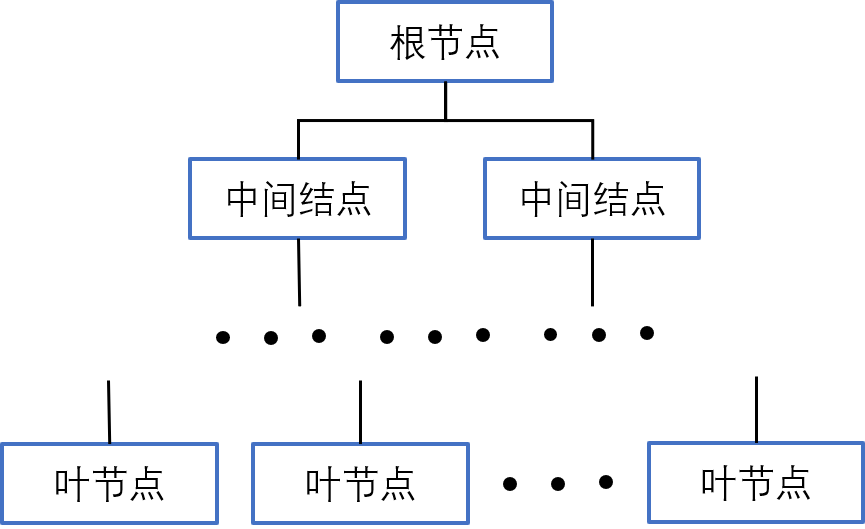
\includegraphics[width=0.6\linewidth]{rtmq/rtmq_nodes_and_leaves_structure}
\end{figure}

RTMQ(用于量子物理实验的实时微系统,RealTime Microsystem for Quantum physics)架构主要用于基于FPGA或ASIC的兼具通用计算和高精度时序控制能力的微系统。系统的整体结构为树状结构,如图\ref{fig:rtmq_nodes_and_leaves_structure}所示,系统包含一个根节点,多个中间结点和多个叶节点;根节点通过网络、USB等方式与控制计算机相连。不同节点可位于同一PCB上,亦可位于不同PCB上。

\begin{figure}
    \centering
    \caption[RTMQ系统架构节点示意图]{RTMQ系统架构节点示意图\label{fig:rtmq_board_overal_structure}}
    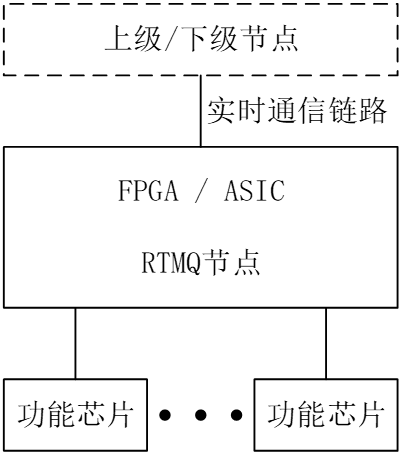
\includegraphics[width=0.4\linewidth]{rtmq/rtmq_board_overal_structure}
\end{figure}

一般而言一个板卡具有如图\ref{fig:rtmq_board_overal_structure}所示的结构,板卡上的FPGA或ASIC包含一个RTMQ节点,RTMQ节点通过控制FPGA或ASIC的输入输出与数模/模数转换等各类功能芯片进行交互以实现所需功能,同时通过实时通信链路与其上级和下级节点连接。

\begin{figure}
    \centering
    \caption[RTMQ系统架构节点内部模块示意图]{RTMQ系统架构节点内部模块示意图\label{fig:rtmq_board_inner_structure}}
    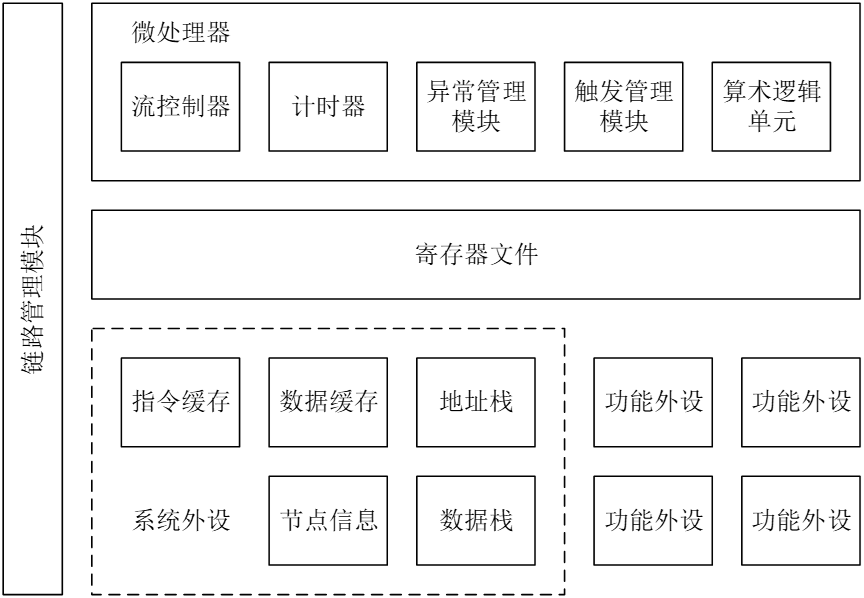
\includegraphics[width=1.0\linewidth]{rtmq/rtmq_board_inner_structure}
\end{figure}

一个RTMQ节点的内部模块儿如图\ref{fig:rtmq_board_inner_structure}所示,包含一个32位的微处理器、一个寄存器文件、一系列外设模块和一个链路管理模块。其中微处理器包含流控制器、计时器、异常管理模块、触发管理模块和算术逻辑单元5个子模块;寄存器文件包含多个寄存器;外设可分为系统外设和功能外设,系统外设包括指令缓存、数据缓存、节点信息只读存储器以及地址栈和数据栈,功能外设用于实现具体的逻辑或时序功能,可包含多个。

RTMQ架构中包含的微处理器可受指令控制进入挂起状态,而挂起状态可受计时器或触发管理模块的控制恢复正常运行,如此,微处理器的指令流便可以按一定的时间间隔对齐或与外部信号对齐。同时,节点中的系统外设和功能外设的行为受关联寄存器的读写控制,即微处理器的指令与系统各模块的功能和时序有严格的对应关系。因此,本发明提供的架构可实现实时控制与通用计算在指令流层面的结合。
而配置指令插入中断的机制确保了节点对其下级节点的绝对控制,即使下级节点的微处理器处于挂起状态,依然不受影响。配置指令插入中断配合具有确定通信延迟的实时通信链路系统,即可实现时序确定的跨节点的即时反馈控制。

此外,RTMQ架构中每个节点都具有通用计算和时序控制能力,如此,大多数通用计算和时序生成都可以在叶节点或较近的中间结点完成,对于大规模系统不存在拥塞的问题,具有良好的可扩展性。


\section[测控硬件组成]{测控硬件组成}
\textcolor{red}{
1. 展示实物板卡照片;}

RTMQ测控板实物图如图\ref{fig:rtmq_board_real}所示。
\begin{figure}
    \centering
    \caption[RTMQ测控板实物图]{RTMQ测控板实物图\label{fig:rtmq_board_real}}
    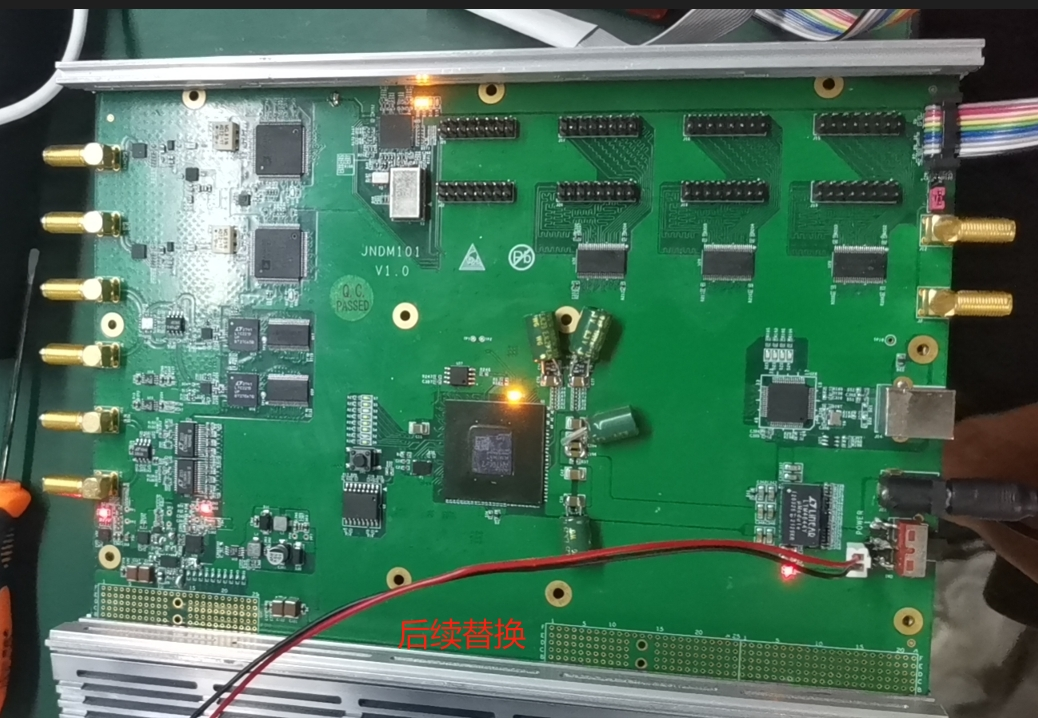
\includegraphics[width=1.0\linewidth]{rtmq/rtmq_board_real}
\end{figure}

\textcolor{red}{
2. 结合照片给出主要器件清单及其介绍(参考专利:一种量子物理实验平台的实时测控系统架构);}



\section[软件API]{软件API}
\textcolor{red}{
1. 介绍软件API的功能和使用(可选,根据情况看吧,怎么介绍还没想好);}


\section[基于FPGA的数字超前进位加法器]{基于FPGA的数字超前进位加法器}
% \textcolor{red}{
% 1. 介绍数字加法器功能、逻辑图、Vivado中的实现、局限性;}

\subsection[加法器]{加法器}


加法器是一种用于执行加法运算的装置,在数字系统中有着广泛的用途。以下是几种常见的加法器结构:
\begin{itemize}
    \item 串行进位加法器(Carry Ripple Adder,CRA):这是最简单、最基本的加法器结构;
    \item 进位跳跃加法器(Carry Skip Adder,CKA);
    \item 进位选择加法器(Carry Select Adder,CSA);
    \item 超前进位加法器(Carry Lookahead Adder,CLA);
    \item 并行前缀加法器(Parallel Prefix Adder,PPA);
\end{itemize}
 
不同的加法器结构具有不同的性能和特点,在实际应用中,需要根据具体需求选择合适的加法器结构。

\subsection[超前进位加法器]{超前进位加法器\label{section:carray_lookahead_adder}}

加法器是构成运算器的基本部件,是构成乘法器、滤波器、数字PID等的基础和重要组成部分。量子测控系统要求高速的运算以实现对量子比特的精准调控,为提高运算速度,加法器一般都采用超前进位或先行进位方式。下面我将以超前进位加法器为例,介绍它的原理和在FPGA中的实现。

超前进位加法器指电路进行二进制加法运算时,通过快速进位电路同时产生除最低位全加器外的其余所有全加器的进位信号,无需再由低位到高位逐位传递进位信号,从而消除了串行进位加法器逐位传递进位信号的时间,提高了加法器的运算速度。

简单来说就是先用初始数据将各个进位都算出来,然后在经过一级全加器得出各个位的数据结果。

对于一个全加器,它的真值表如表\ref{tb:carry_ripple_adder}。其中$i_c$表示输入来自前一位的进位,$i_a, i_b$表示输入当前位待相加的两个数,$o_d$表示加法器输出结果的数据位;$o_c$表示加法器输出的向下一位的进位。
\begin{table}
    \centering
    \caption[串行进位加法器真值表]{串行进位加法器真值表。$i_c$表示输入来自前一位的进位;$i_a, i_b$表示输入当前位待相加的两个数;$o_d$表示加法器输出结果的数据位;$o_c$表示加法器输出的向下一位的进位。\label{tb:carry_ripple_adder}}
    \begin{tabular}{C{1.5cm}C{1.5cm}C{1.5cm}|C{1.5cm}C{1.5cm}}
        \toprule 
        \multicolumn{3}{c}{\textbf{Input}} & \multicolumn{2}{c}{\textbf{Output}}\\
        \toprule
        $i_c$ & $i_a$ & $i_b$ & $o_d$ & $o_c$\\
        \hline
        0 & 0 & 0 & 0 & 0 \\
        1 & 0 & 0 & 1 & 0 \\
        0 & 0 & 1 & 1 & 0 \\
        1 & 0 & 1 & 0 & 1 \\
        0 & 1 & 0 & 1 & 0 \\
        1 & 1 & 0 & 0 & 1 \\
        0 & 1 & 1 & 0 & 1 \\
        1 & 1 & 1 & 1 & 1 \\
        \bottomrule
    \end{tabular}
\end{table}

上述串行加法器的布尔表达式为:
\begin{align}
    o_d=&i_c \oplus i_a \oplus i_b\\
    Case1:
    o_c=&(i_a \cdot i_b) + (i_a \cdot i_c) + (i_b \cdot i_c)\\
    Case2:
    o_c=&i_c \cdot (i_a \oplus i_b) + i_a \cdot i_b\\
    Case3:
    o_c =& i_c \cdot (i_a + i_b) + i_a \cdot i_b
\end{align}

其中“$\oplus$”表示“异或”运算,“$\cdot$”表示“与”运算,“$+$”表示“或”运算。

\begin{figure}
    \centering
    \caption[串行进位加法器的FPGA实现结构图]{串行进位加法器的FPGA实现结构图\label{fig:carry_ripple_adder}(Vivado)}
    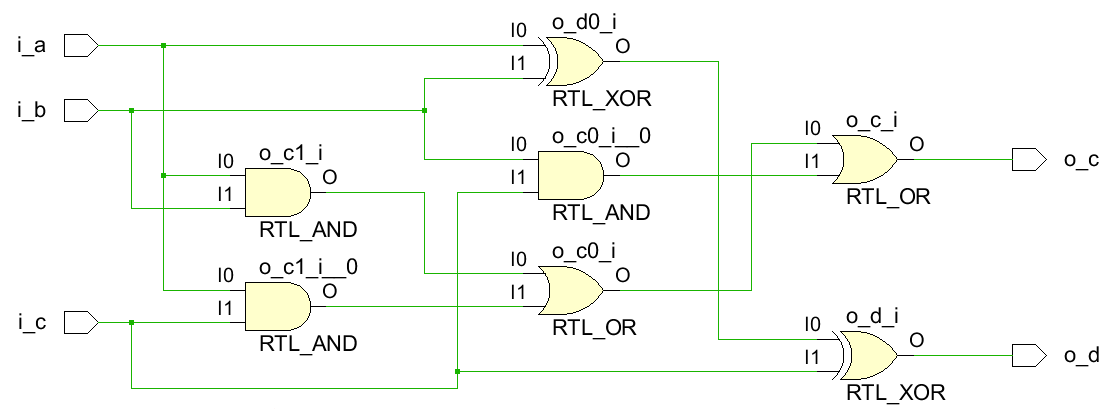
\includegraphics[width=0.9\linewidth]{rtmq/adder_case1}
    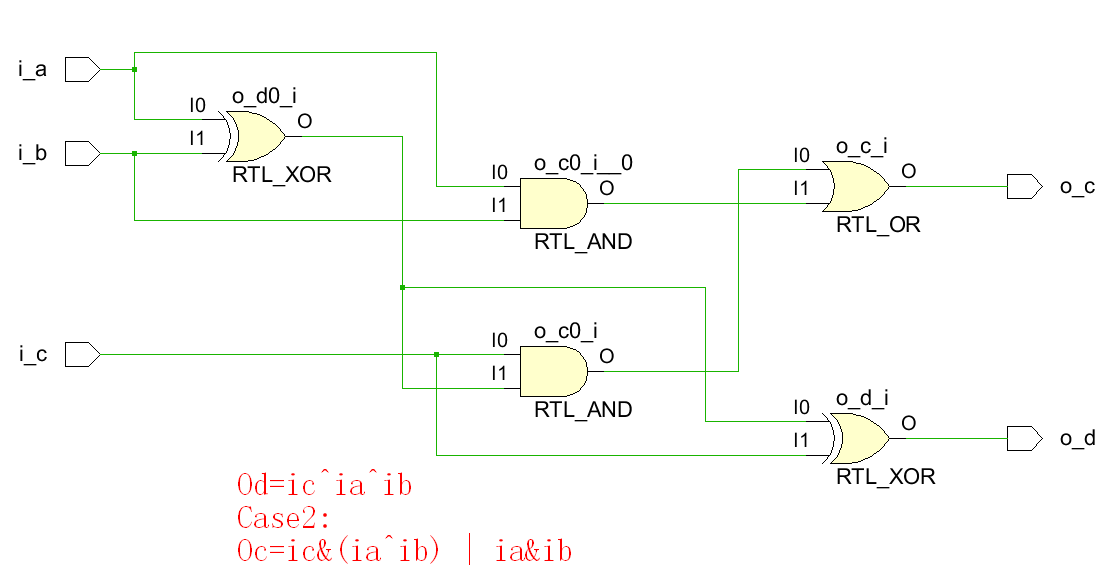
\includegraphics[width=0.9\linewidth]{rtmq/adder_case2}
    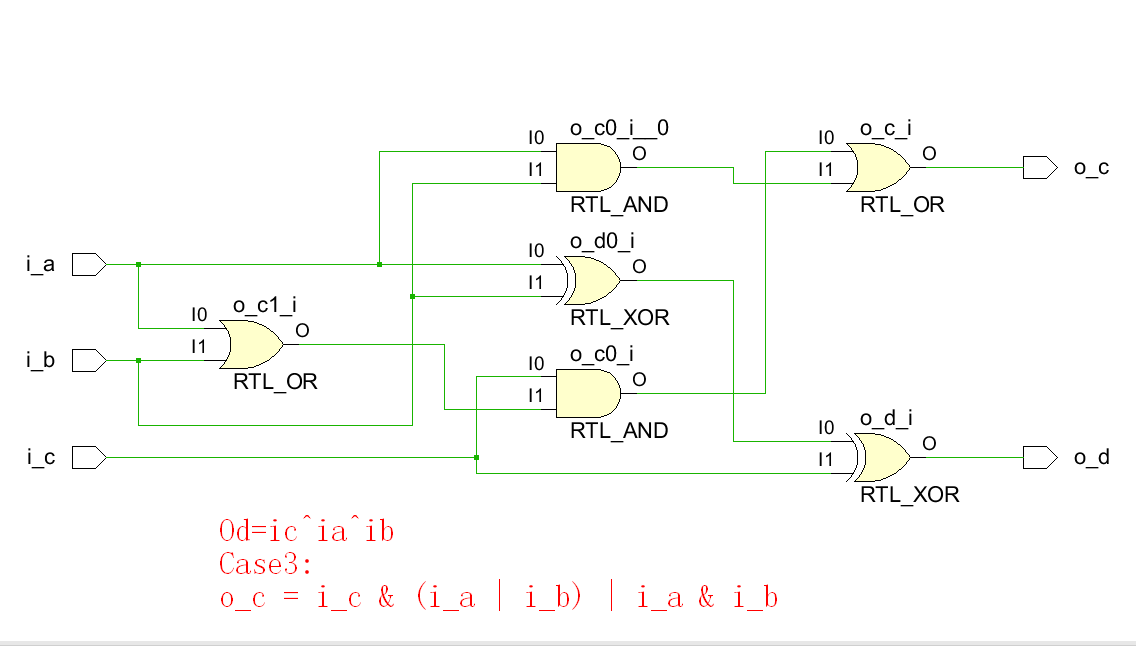
\includegraphics[width=0.9\linewidth]{rtmq/adder_case3}
\end{figure}

三种串行进位加法器实现的结构图如图\ref{fig:carry_ripple_adder}所示。从结果可以看到,第一种写法用了7个元件,输入到输出需要三级门电路得到结果;第二种写法用了5个器件,输入到输出需要三级门电路得到结果;第三种写法用了6个元件,输入到输出需要三级门电路得到结果;从器件数量角度优选地应该使用第二种写法,具体还取决于系统可用的元器件情况。可以看出当前位对下一位的数据和进位逻辑如下:

\begin{align}
    d_i =& a_i\oplus b_i \oplus c_i\\
    c_{i+1}=& a_i \cdot b_i +(a_i \oplus b_i)\cdot c_i = G_i + (P_i)\cdot c_i
\end{align}

其中$G_i=a_i \cdot b_i$是生成信号,$P_i=a_i \oplus b_i$是传播信号。如果想要消除进位依赖,那么进位$c_{i+1}$的表达式就不能有$c_i, c_{i-1}, \dots, c_i$项,$c_0$项为初始赋予不需要替换。这里考虑四位超前进位加法器设计如下:

\begin{align}
    c_0 &= c_0\\
    c_1 &= G_0 + P_0 c_0\\
    c_2 &= G_1 + P_1 c_1 = G_1+P_1 (G_0+P_0 c_0 )=G_1+P_1 G_0+P_1 P_0 c_0\\
    c_3 &=G_2+P_2 c_2=G_2+P_2 (G_1+P_1 G_0+P_1 P_0 c_0 )\\
    &=G_3+P_3 G_2+P_3 P_2 G_1+P_3 P_2 P_1 P_0 c_0\\
    c_5 &=G_4+P_4 c_4=G_4+P_4 (G_3+P_3 G_2+P_3 P_2 G_1+P_3 P_2 P_1 P_0 c_0 )\\
    \dots\\
    c_{i+1} &=G_i+P_i G_{i-1}+P_i P_{i-1} G_{i-2}+ \dots +\prod_0^i P_j \cdot c_0
\end{align}

从中可见,对于第$i+1$位进位的计算$P_i$要参加$i+1$组计算。超前进位加法器的FPGA实现结构图如图\ref{fig:ahead_adder_4bits}所示。

\begin{figure}
    \centering
    \caption[4位超前进位加法器的FPGA实现结构图]{4位超前进位加法器的FPGA实现结构图(Vivado)\label{fig:ahead_adder_4bits}}
    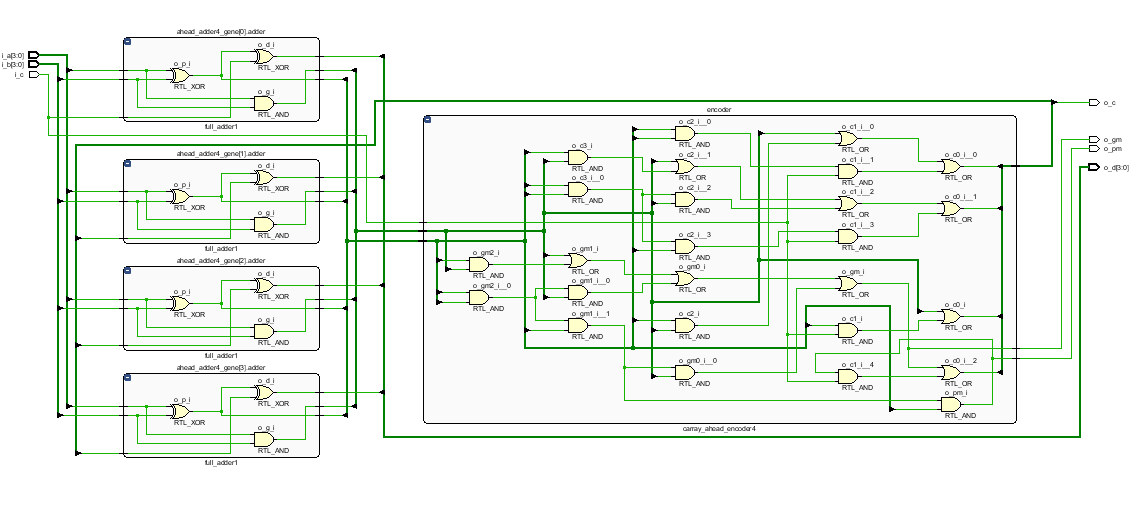
\includegraphics[width=1.0\linewidth]{rtmq/ahead_adder_4bits}
\end{figure}

按照上述规律进行拓展,可以依次得到需求位数的超前进位加法器,比如8位(附录图\ref{fig:ahead_adder_8bits})、16位(附录图\ref{fig:ahead_adder_16bits})、32位(图\ref{fig:ahead_adder_32bits})等。值得注意的是,理论上使用超前进位方式可以实现任意位数的加法器,并且实现的加法器只需要两级流水线就可以得到最终结果。不过实际上高速数字电路的延时不仅有流水线延时,还有器件延时。可以看到超前进位加法器从4位(图\ref{fig:ahead_adder_4bits})到32位(图\ref{fig:ahead_adder_32bits}),在超前进位计算的逻辑有了相当程度的复杂化了。受到器件压时延的限制,我们无法超前计算无限位数的超前进位$c_{\infty}$。

\begin{figure}
    \centering
    \caption[32位超前进位加法器的FPGA实现结构图]{32位超前进位加法器的FPGA实现结构图(Vivado)\label{fig:ahead_adder_32bits}}
    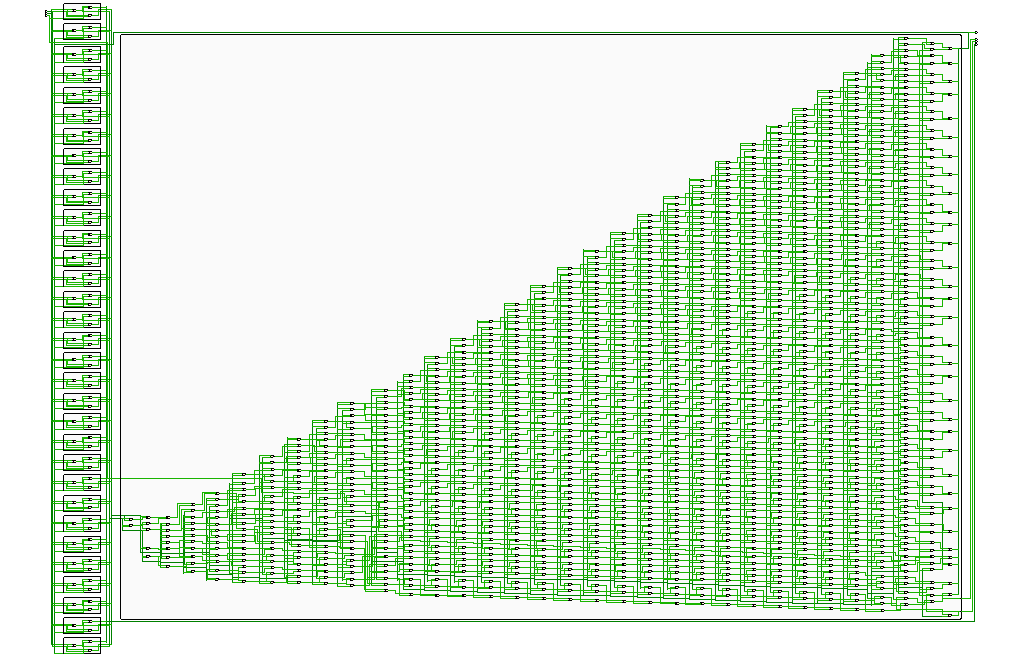
\includegraphics[width=1.0\linewidth]{rtmq/ahead_adder_32bits}
\end{figure}
\begin{figure}
    \centering
    \caption[用两个32位超前进位加法器拓展为一个64位加法器]{用两个32位超前进位加法器拓展为一个64位加法器(Vivado)\label{fig:adder_64bits}}
    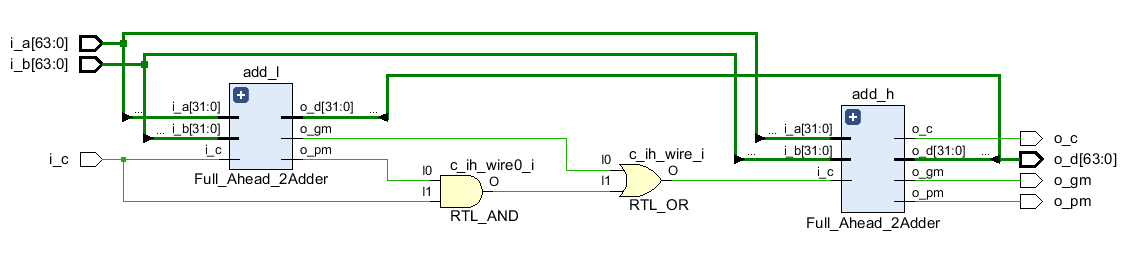
\includegraphics[width=1.0\linewidth]{rtmq/adder_64bits}
\end{figure}

一般情况下32位加法器就足够用了,比如RTMQ系统就是采用32位运算的。如果需要更高位数的加法器可以继续向上拓展,也可以考虑用串行进位加法器的思想对超前进位加法器进行拓展。

如图\ref{fig:adder_64bits}所示,这里用了两个32位加法器添加了一级流水线,拓展为了一个64位的加法器。用这种方式可以满足一些特殊的更高位数加法器的实现。不过,在流水线时延上要做出一点妥协。







\newpage
\section[基于FPGA的数字Booth乘法器]{基于FPGA的数字Booth乘法器\label{section:booth_multiplier}}
% \textcolor{red}{
% 1. 介绍数字Booth乘法器功能、逻辑图、Vivado中的实现、优势;}
布斯(Booth)乘法器是一种对乘数进行重新编码,以减少乘法运算中所需的加法次数的乘法器。它由布斯夫妇于 1950 年发明,因硬件实现简单、所需硅片面积较小、能够显著提高乘法运算速度而被广泛采用。

Booth乘法器通过相加和相减的操作计算补码数据的乘积。该算法对乘数从低位开始判断,根据后两个数据位的情况决定进行加法、减法还是仅仅进行移位操作。
在计算两个补码相乘时,会将上一轮编码产生的进位与当前轮编码进行相加,然后再进行移位操作。通过这种方式,布斯乘法器可以减少乘法运算中所需的加法次数,从而提高计算速度。

Booth乘法器在数字信号处理、计算机算术、密码学等领域中具有广泛的应用\cite[]{Jigjidsuren_Badarch_Sukhbaatar_Namsrai_2021}。在RTMQ系统中有关的乘法运算基本都是以Booth乘法器来实现的。下面将介绍它的原理和实现。

\subsection[乘法基本]{乘法基本}
不采用任何优化算法的乘法过程可以用列竖式乘法来表示。从乘数的低位开始,每次取一位与被乘数相乘,乘积作为部分积(Partial Product, PP)暂存。乘数的全部有效位乘完后,再将所有部分积(PP0-PPx)按照对应乘数位的相应权重错位相加,得到最后的乘积。如图\ref{fig:multiple_process}所示,左图和右图分别展示了十进制数和二进制数的无优化算法乘法过程,可见二进制乘法和十进制乘法本质上并无差别。

\begin{figure}
    \centering
    \caption[十进制数和二进制数的无优化算法乘法过程]{十进制数和二进制数的无优化算法乘法过程\label{fig:multiple_process}}
    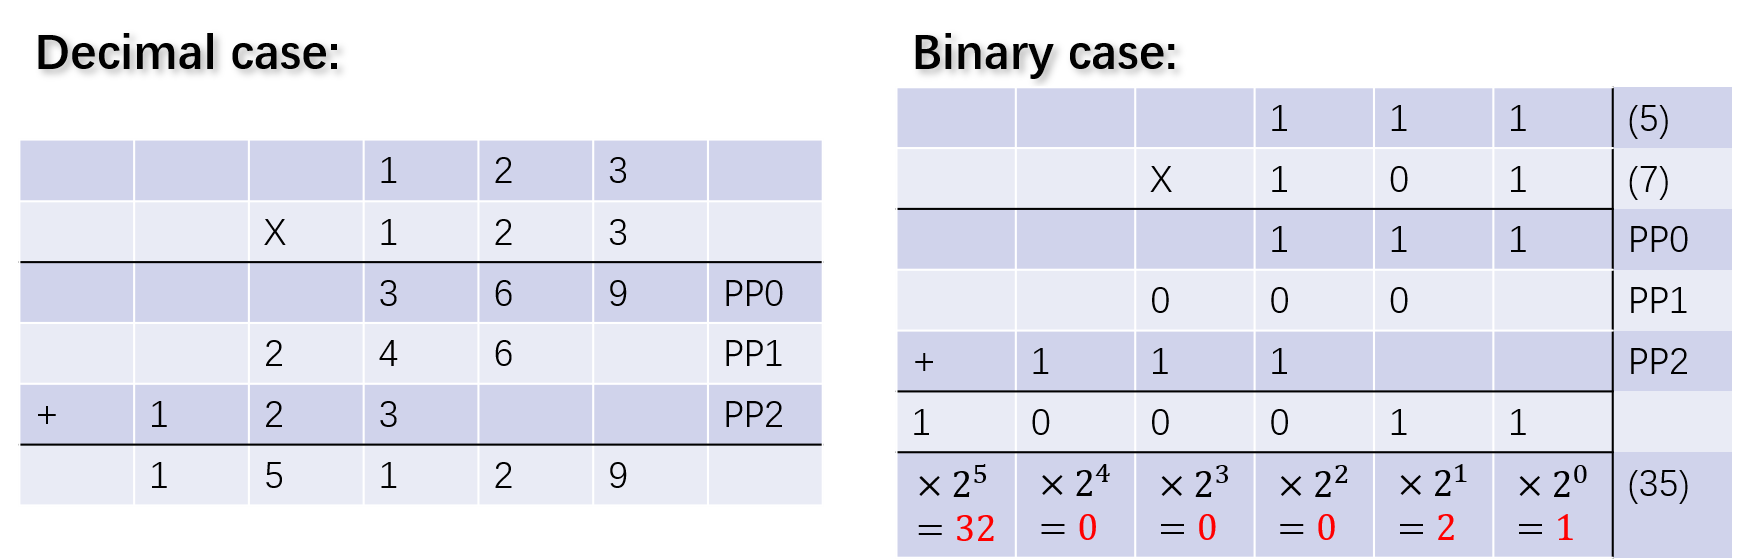
\includegraphics[width=1.0\linewidth]{rtmq/multiple_process}
\end{figure}

如果将乘法过程表示成通式,比如4位乘法器,如图\ref{fig:multiple_process_general}所示。这样原始的乘法在设计上是可以实现的,但在工程应用上几乎不会采用,在时延与面积上都需要优化。一个$n_1=n_2=N$位的乘法运算,需要产生$N$个部分积,并对它们进行全加处理,位宽越大,部分积个数越多,需要的加法器也越多,加法器延时也越大,这对高速芯片来说是很不有好的。实际上乘法过程拆解开来就是获得部分积和处理部分积相加的过程。由于在二进制中获得部分积的过程可以通过简单的移位来实现,因此针对乘法运算的优化,主要就集中在两个方面:一是减少部分积的个数,二是减少加法器带来的延时。

\begin{figure}
    \centering
    \caption[4位乘法过程通式]{4位乘法过程通式\label{fig:multiple_process_general}}
    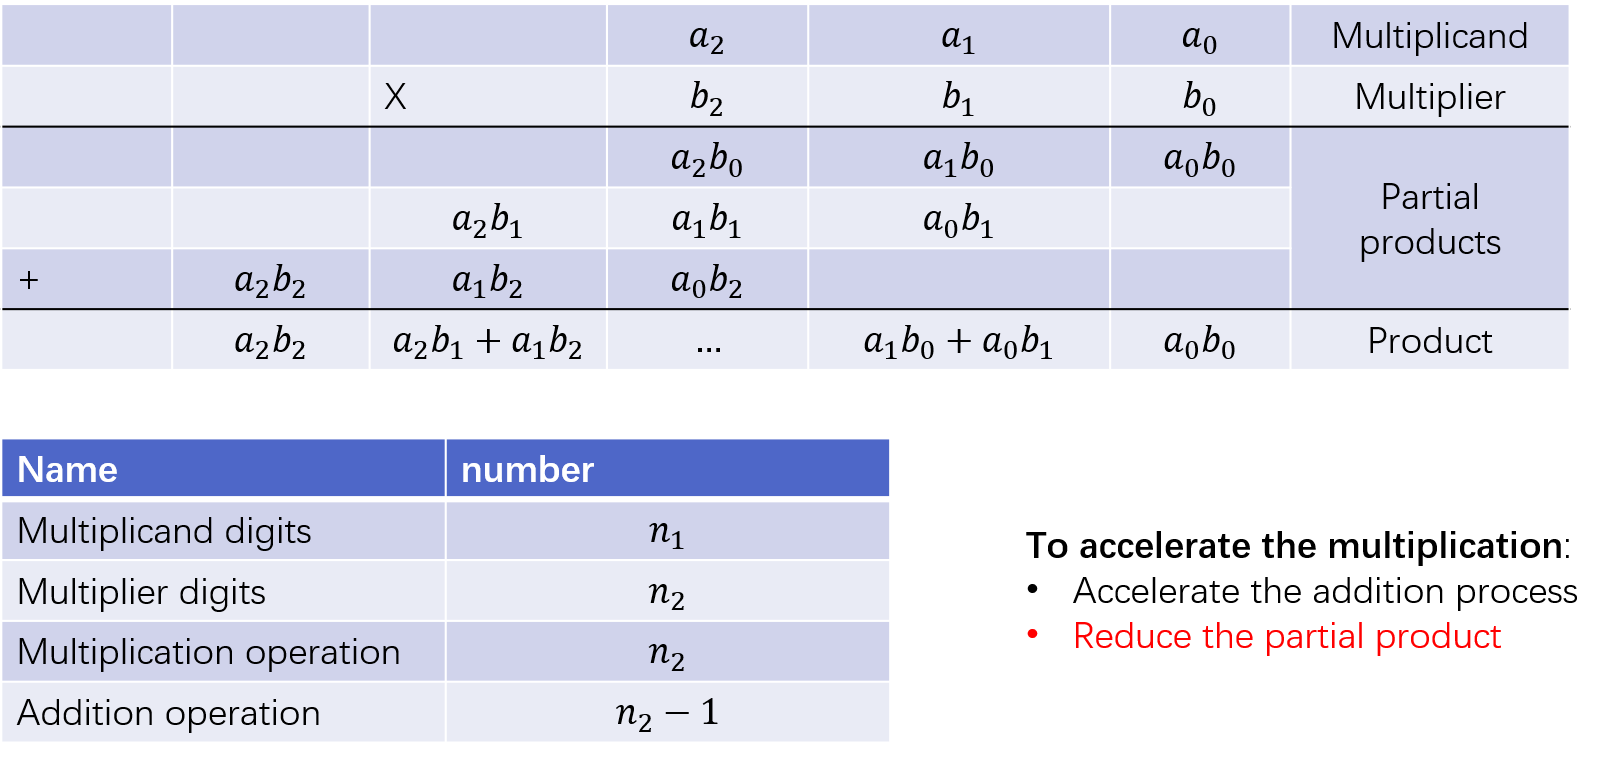
\includegraphics[width=1.0\linewidth]{rtmq/multiple_process_general}
\end{figure}

\subsection[改进的Booth编码]{改进的Booth编码}

任意$n$比特的有符号数可以表示为:
\begin{align}
    y=&-2^{n-1} y_{n-1}+2^{n-2} y_{n-2}+\\
    &…+2^2 y_2+2^1 y_1+2^0 y_0+y_{-1}\label{eq:binary_number_expression}
\end{align}

其中$-2^(n-1) y_(n-1)$是符号,$y_(-1)=0$是添加的辅助比特。公式\ref{eq:binary_number_expression}可以被进一步变形为:

\begin{align}
    y=&-2^{n-1} y_{n-1}+(2^{n-2} y_{n-2}+2^{n-2} y_{n-2} )-2^{n-2} y_{n-2}+…+(2^2 y_2\\
    &+2^2 y_2 )-2^2 y_2+(2^1 y_1+2^1 y_1 )-2^1 y_1+(2^0 y_0+2^0 y_0 )-2^0 y_0+y_{-1}\\
    =&-2^{n-1} y_{n-1}+(2^{n-1} y_{n-2} )-2^{n-2} y_{n-2}+\\
    &…+(2^3 y_2 )−2^2 y_2+(2^2 y_1 )-2^1 y_1+(2^1 y_0 )-2^0 y_0+y_{-1}\\
    =&2^{n-1} (-y_{n-1}+y_{n-2} )+2^{n-2} (-y_{n-2}+y_{n-3} )+\\
    &…+2^1 (-y_1+y_0 )+2^0 (-y_0+y_{-1})\label{eq:binary_number_expression1}
\end{align}

通过公式\eqref{eq:binary_number_expression1}可以发现,多项表达式的项数变成了原来的一半。原二进制数从LSB(最低位)开始,以三位为一组(第一组最低位需补一个附加位即$y[-1]$,附加值为$0$),相邻组之间重叠一位(低位组的最高位与高位组的最低位重叠),构成新的多项式因子,这就是\emph{改进的布斯编码}方式。

两个二进制数乘,如果对乘数进行公式\eqref{eq:binary_number_expression1}所示的改进型布斯编码,则得出的部分积个数相较直接相乘可以减半。比如,两个32位数相乘,不做布斯编码直接相乘,则有32个部分积需要累加,而采用 式3 的编码方式对其中一个因数进行变换后,将只有16个部分积需要累加。

由公式\eqref{eq:binary_number_expression1}可知,组成多项式因子的每连续三位之间的关系是完全相同的,二进制中每一位的数值非0即1,由此可以列出相邻三位所有取值组合下,其对应多项式因子的值。设某乘法运算中,被乘数为$X$,乘数为$Y$,$Y_{i+1},\ Y_{2i},\ Y_{2i-1}$分别为$Y$的连续三位,其中$i$为自然数$N$,$PP_i$为$i$不同取值下对应的部分积,对$Y$进行改进的布斯变换后再与$X$相乘,则可以有如表\ref{tb:booth_lookup_table}推算关系。

\begin{table}
    \centering
    \caption[基4布斯编码查找表]{基4布斯编码查找表\label{tb:booth_lookup_table}}
    \begin{tabular}{C{2cm}C{2cm}C{2cm}|C{2cm}}
        \toprule 
        \multicolumn{3}{c}{\textbf{Input}} &\textbf{Output}\\
        \toprule
        $Y_{2i+1}$ & $Y_{2i}$ & $Y_{2i-1}$ & $PP_i$\\
        \hline
        0 & 0 & 0 & 0 \\
        1 & 0 & 0 & X\\
        0 & 0 & 1 & X\\
        1 & 0 & 1 & 2X\\
        0 & 1 & 0 & -2X\\
        1 & 1 & 0 & -X\\
        0 & 1 & 1 & -X\\
        1 & 1 & 1 & 0\\
        \bottomrule
    \end{tabular}
\end{table}

由此可见,根据乘数每连续三位的值,可以快速推算出其对应的部分积。且在二进制中,乘2操作可以通过左移一位来实现,不需要复杂的计算,电路实现非常简单,通过此方法,解决了硬件乘法优化的第一个方面,简化和减少部分积的生成。作为改进型布斯编码中最基础的一种,它被称之为基4布斯编码。基4编码相当于每次用乘数的两位与被乘数相乘产生部分积,从而使部分积个数减少一半,也可以看成是将乘数转化为4进制表达,故称为基4(Radix-4 Booth Encoding)。采用基4布斯编码的乘法相较于传统乘法运算,优化效果已经很明显且易于实现,可以满足大部分应用要求,32位乘法器,甚至64位乘法器都可以采用,是比较常用的一种方式。当然,更高阶的布斯编码可以更大程度地减少部分积个数,但因其部分积产生逻辑无法单纯通过移位实现,需要引入加法器等其它运算部件,从这方面来看又削弱了优化效果,需要综合考量选择。

\subsection[进位保留加法器与3-2压缩、4-2压缩]{进位保留加法器与3-2压缩、4-2压缩}
布斯编码解决了乘法优化的第一个方面,通过减少部分积个数从而减少累加器个数,但累加器本身的进位传递延时对电路性能依然存在非常大的影响,所以优化的第二个方面,就是改进部分积累加结构,提升累加性能。如果采用部分积直接相加的方式,因为全加器进位的关系,当前bit的相加结果依赖于它前一bit的进位输出,整个计算过程相当于串行化,位宽越大,延时越大,所以优化的关键就是消除进位链,使运算并行化。

进位保留加法器(Carry Save Adder, CSA)是比较常用的一种优化方式,CSA实际上就是一位全加器,其逻辑表达示如下:


进位保留加法器编码相当于一次接受三个输入,产生两个输出,因此也称为3-2计数器或3-2压缩(3-2编码)。如图\ref{fig:carray_save_adder_clock}所示,运用到乘法器中,通过对若干个部分积按每3个为一组进行CSA计算,然后用同样的方法运用到每级CSA产生的输出上,直到最后一级CSA的两个输出,再用全加器得到最后的部分积累加结果。
\begin{figure}
    \centering
    \caption[进位保留加法器编码(3-2编码)]{进位保留加法器编码(3-2编码)\label{fig:carray_save_adder_clock}}
    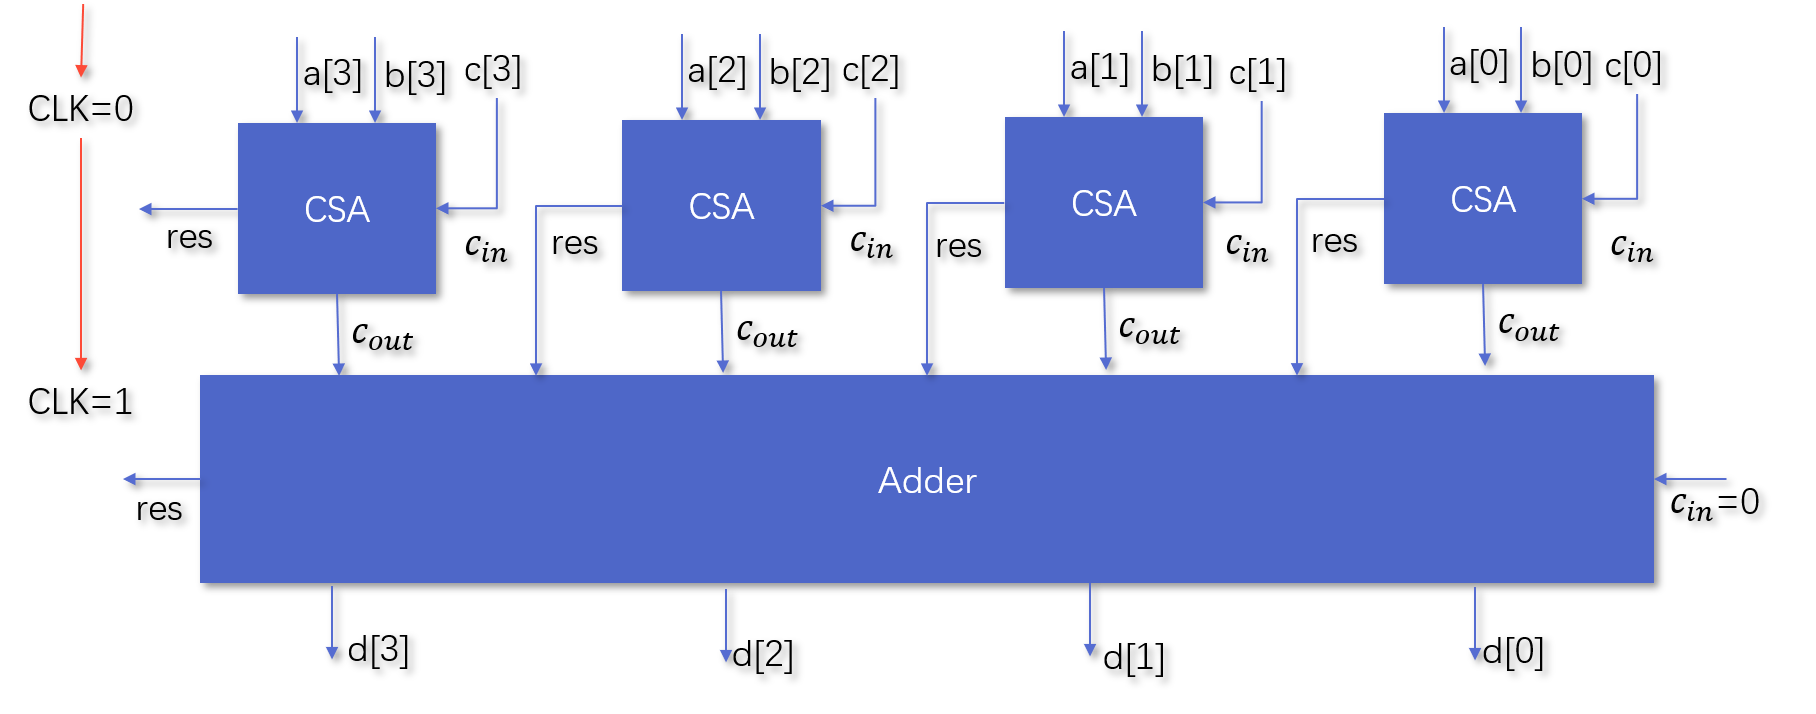
\includegraphics[width=1.0\linewidth]{rtmq/carray_save_adder_clock}
\end{figure}

相较于3-2压缩,还有一种压缩率更高的方式叫4-2压缩(编码),或称为5-3计数器。顾名思义,就是有5个输入端,产生3个输出,运用到加法上,可以实现同时计算四个加数,生成对应的结果与进位值。设5-3计数器的5个输入分别为$I[0], I[1], I[2], I[3], C_i$,3个输出端分别为$ D, C, C_o$,则它们之间满足如下代数关系:
\begin{align}
    D+C\times 2+C_o\times 2=I_0+I_1+I_2+I_3+C_i\label{eq:encoder_5to3}
\end{align}
根据公式\eqref{eq:encoder_5to3},可以推算出相应的真值表如表\ref{tb:encoder_5to3}所示。
\begin{table}
    \centering
    \caption[4-2压缩器真值表]{4-2压缩器真值表\label{tb:encoder_5to3}}
    \begin{tabular}{C{1.5cm}|C{4cm}|C{1.5cm}C{1.5cm}C{1.5cm}}
        \toprule 
        \multicolumn{2}{c}{\textbf{Input}} &\multicolumn{3}{c}{\textbf{Output}}\\
        \toprule
        $C_i$ & $I_0+I_1+I_2+I_3$ & $C_0$ & $C$ & $D$\\
        \midrule
        \multirow{5}{3cm}{0} & 0 & 0 & 0 & 0 \\
        & 1 & 0   & 0     & 1 \\
        & 2 & 0/1 & 1/0   & 0 \\
        & 3 & 0/1 & 1/0   & 1 \\
        & 4 & 1   & 1     & 0\\
        \hline
        \multirow{5}{3cm}{1} & 0 & 0 & 0 & 1\\
        & 1 & 0/1 & 1/0   & 0 \\
        & 2 & 0/1 & 1/0   & 1 \\
        & 3 & 1   & 1     & 0 \\
        & 4 & 1   & 1     & 1 \\
        \bottomrule
    \end{tabular}
\end{table}

输出与输入之间的逻辑经化简最后可表达示为:
\begin{align}
    D=&I_0\oplus I_1\oplus I_2\oplus I_3 \oplus C_i\\
    C=&((I_0\oplus I_1\oplus I_2\oplus I_3)\cdot C_i)\\
    &+\neg ((I_0\oplus I_1\oplus I_2\oplus I_3)+\neg((I_0\cdot I_1)+(I_2\cdot I_3)))\\
    C_o=&(I_0+I_1)\cdot(I_2+I_3)
\end{align}
\subsection[Booth乘法器的硬件实现]{Booth乘法器的硬件实现}
下面以一个$8\times 8$的乘法器为例,介绍运用上述介绍设计和实现Booth乘法器的方法,更大位宽的乘法器可以通过类似的方法拓展得到。

前面对算法原理的论述中,没有提及有符号数和无符号数,但在设计的时候,则需要考虑有符号数与无符号数的区别。实际上布斯编码是带符号位的,也就是它的编码方式是建立在有符号数基础之上,从多项式1的最高次项也可以看出来。所以,采用布斯编码的乘法器是一种有符号数乘法器,或者说补码乘法器(原码与补码的关系不在此文讨论范围)。为了使乘法器能够兼容无符号数计数,可以对乘数扩展一位符号位,当计算无符号数时,该位为0;当计算有符号数时,该位等于扩展前的符号位。如此会导致增加一个部分积,但带来的便利是对两种不同性质的数可以采用完全一样的计算方式,下面的设计实例遵循此方式进行。

设$A[8:0], B[8:0]$分别为乘法器的两个输入,以$A$为被乘数,$B$为乘数。$A[8]$和$B[8]$为兼容无符号数扩展的符号位。

首先,根据前文内容,对乘数B以基4的方式进行改进型布斯编码,即从LSB开始,以每3bit为一组进行分组,每相邻两组之间的最高位与最低位重合(红色位),LSB的右边还需增加一个附加位,定义为$B[-1]$,值为零。如图\ref{fig:booth_multiplier_8bits_basic1}所示。

\begin{figure}
    \centering
    \caption[8位Booth乘法器编码表]{8位Booth乘法器编码表\label{fig:booth_multiplier_8bits_basic1}}
    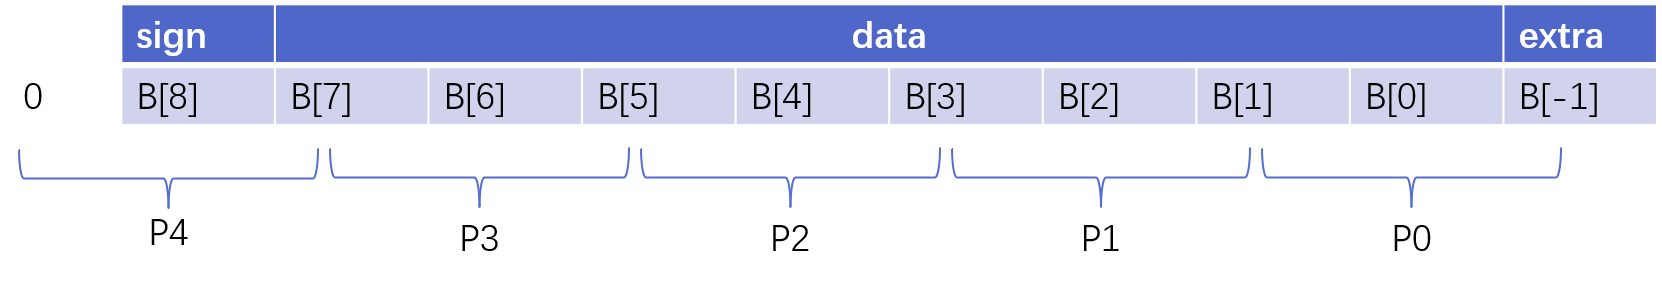
\includegraphics[width=1.0\linewidth]{rtmq/booth_multiplier_8bits_basic1}
\end{figure}


$B[1:-1]$为第1组,$B[3:1]$为第2组,$B[5:3]$为第3组,依此类推,一共可划分为5组。其中第5组因为不够3个bit,故在最高位再扩展一位符号位,符号位的扩展并不会改变补码数据的值。根据每组的值和表\ref{tb:booth_lookup_table}的查找关系,可得出对应的部分积,一共产生5个部分积,定义为PP0~PP4。相邻两组部分积之间权重相差4倍,相当于二进制运算中的左移两位,于是可以将部分积按对应权重排列为如图\ref{fig:booth_multiplier_8bits_basic0}形式。
\begin{figure}
    \centering
    \caption[8位Booth乘法器部分积排列表]{8位Booth乘法器部分积排列表\label{fig:booth_multiplier_8bits_basic0}}
    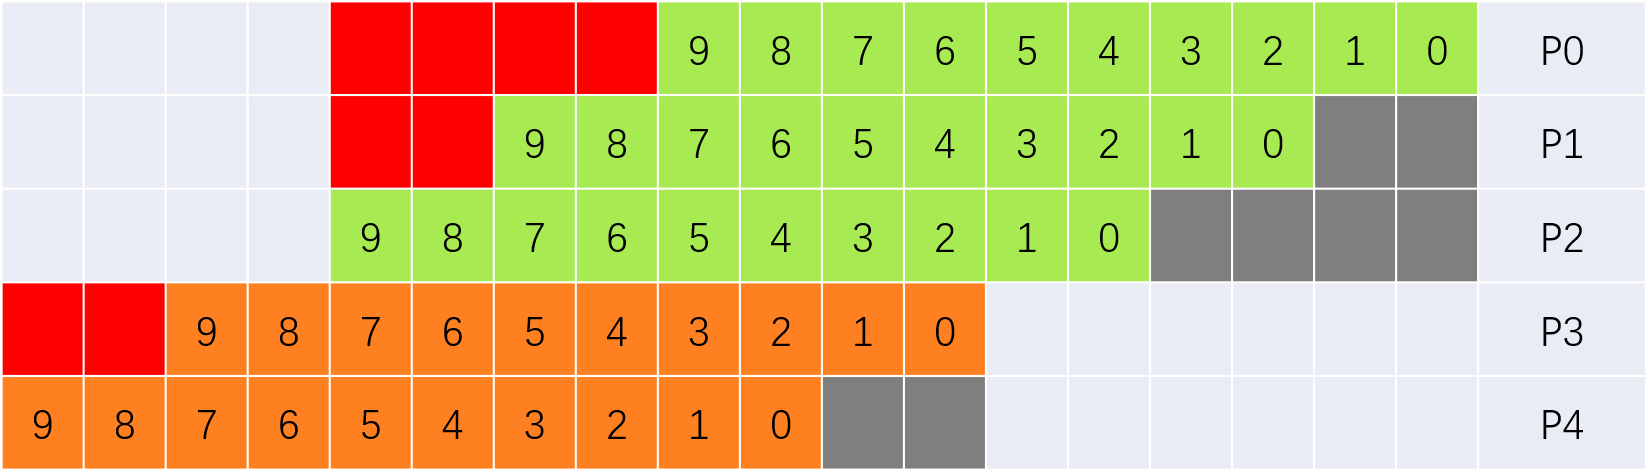
\includegraphics[width=1.0\linewidth]{rtmq/booth_multiplier_8bits_basic0}
\end{figure}

\subsection[3-2压缩器组建加法树]{3-2压缩器组建加法树}
部分积生成后,即可组建加法树。加法树的构成采用3-2压缩方式,8位Booth乘法器的编码表和加法树如图\ref{fig:booth_multiplier_8bits_basic}所示。

% 8位Booth乘法器的编码表和编程设计图如图\ref{fig:booth_multiplier_8bits_basic}所示。
\begin{figure}
    \centering
    \caption[8位Booth乘法器加法树的构建]{8位Booth乘法器加法树的构建\label{fig:booth_multiplier_8bits_basic}}
    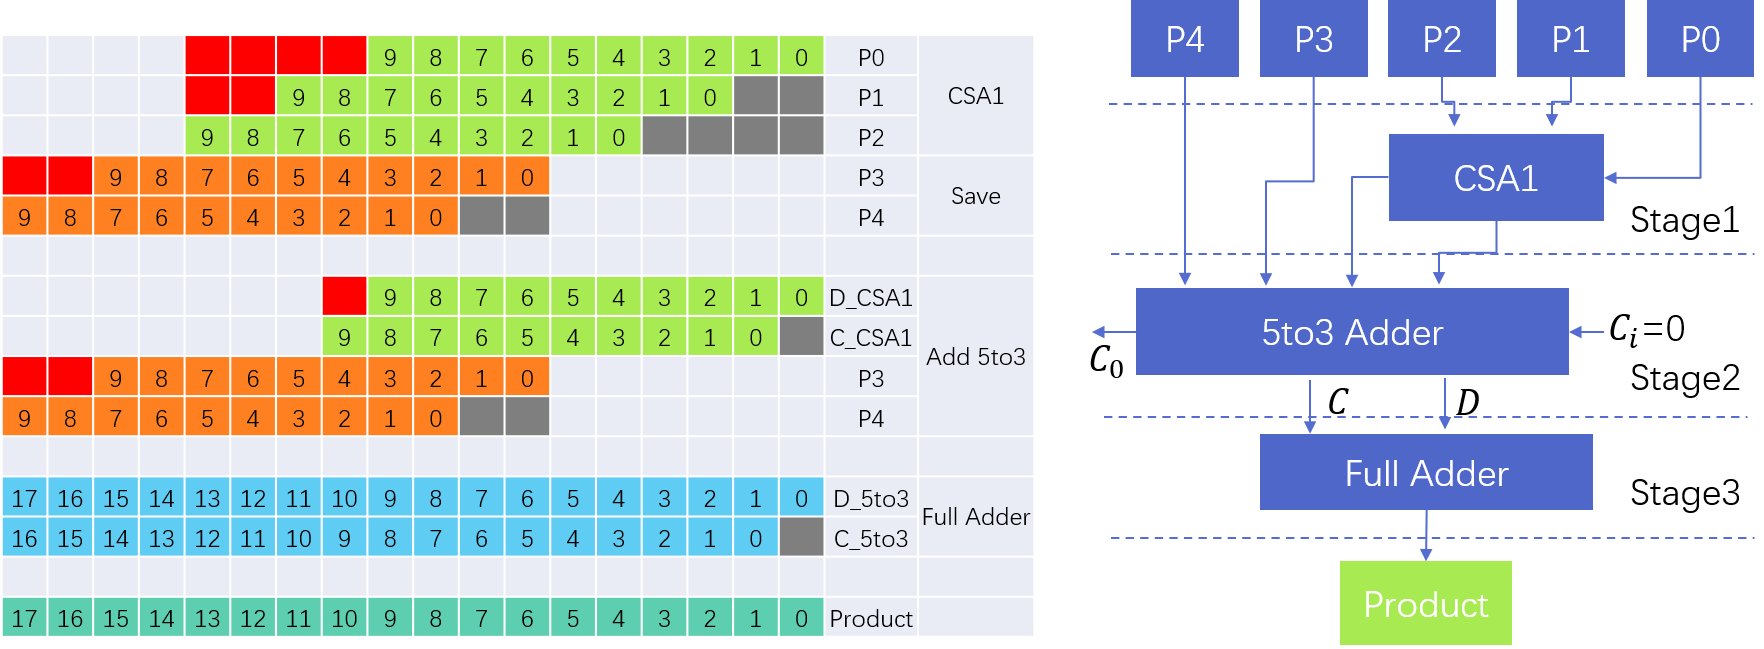
\includegraphics[width=1.0\linewidth]{rtmq/booth_multiplier_8bits_basic}
\end{figure}

5个部分积分别为PP0-PP4,从PP0开始,每三个为一组进行3-2压缩,使用一个3-2压缩器。在第一级中PP0-PP2使用一个3-2加法器,由于P3和P4不足三个输入,在第一级进行保留;第二级中的输入有4个,正好可以采用一个4-2编码器;在第三级中可以直接采用全加器计算得到最终结果。在每个3-2压缩或者4-2压缩的过程中,相邻部分积由于偏移造成的输入不足时,低位补0(图表中灰色填充部分),高位补符号位(图表中红色填充部分)。8位乘法器的正常积结果为16位,因此超过16位的部分可以直接舍弃不参与运算。

综上例子中的$8\times 8$Booth乘法器采用了一个3-2编码器、一个4-2编码器和一个16位全加器,经过3级流水线计算得到最终积。加法树的拓扑可以有很多选择,比如也可以仅采用3-2编码器或者仅采用4-2编码器,一般来说优化的方向是编码级数尽量少、器件尽量少,具体可以根据实际应用进行取舍。

从上面的叙述中可以看出,Booth乘法器的实现重点是要获得一个编码和加法树表,根据加法树表可以绘制出相应的加法树,并进一步在代码中实现。
16位Booth乘法器的编程设计图如图\ref{fig:booth_multiplier_16bits_basic}所示。相应的结构示意图如图\ref{fig:booth_multiplier_16bits_basic_s}所示。
\begin{figure}
    \centering
    \caption[16位Booth乘法器编码和加法树表]{16位Booth乘法器编码和加法树表\label{fig:booth_multiplier_16bits_basic}}
    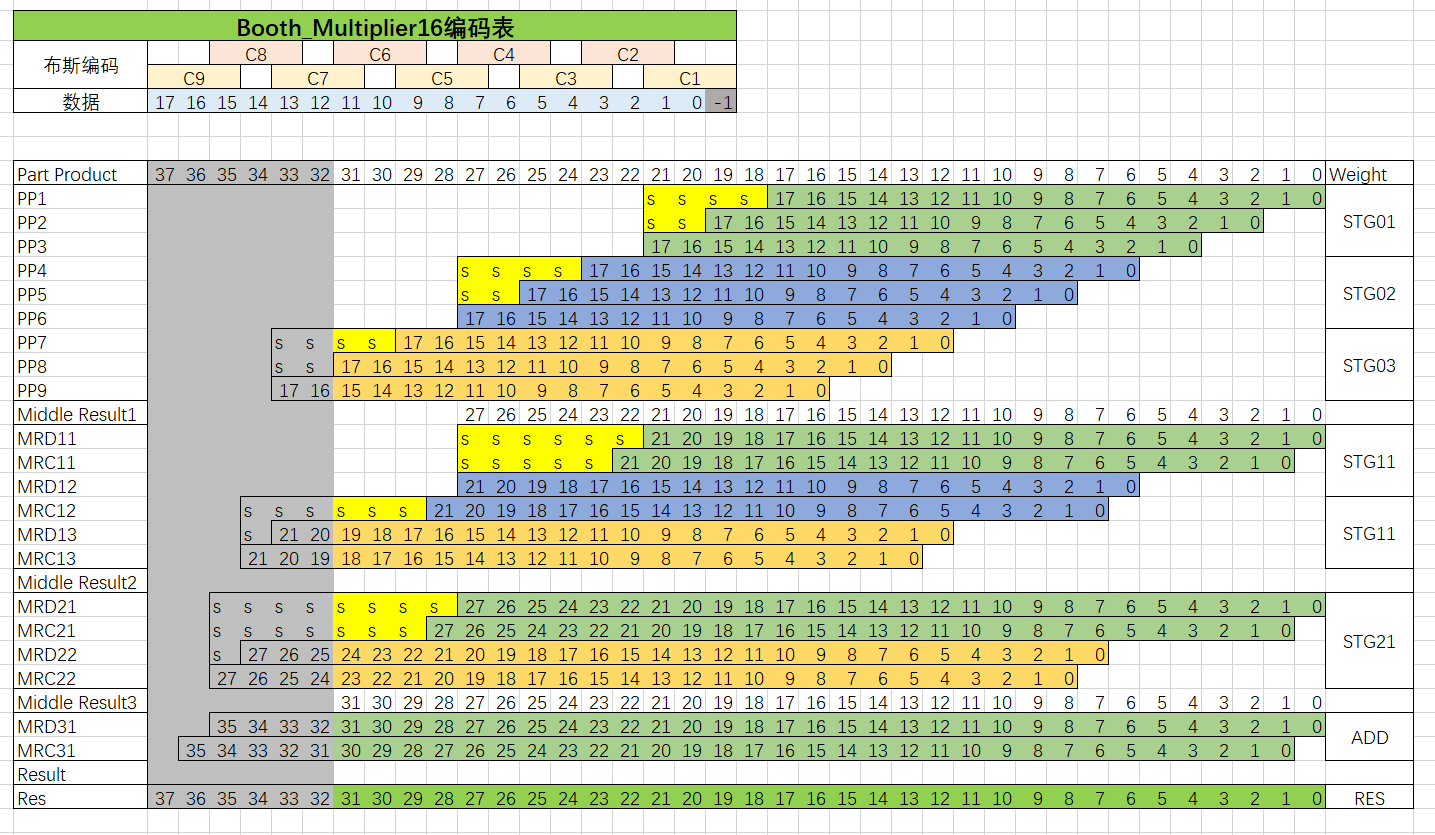
\includegraphics[width=1.0\linewidth]{rtmq/booth_multiplier_16bits_basic}
\end{figure}

\begin{figure}
    \centering
    \caption[16位Booth乘法器结构示意图]{16位Booth乘法器结构示意图\label{fig:booth_multiplier_16bits_basic_s}}
    \includesvg[width=1.0\linewidth]{rtmq/booth_multiplier_16bits_basic_s}
\end{figure}

上述实现的16位Booth乘法器已经可以满足RTMQ系统的基本使用需求了。更高位数的Booth乘法器实现可以依据上述规律进行设计开发。作为扩展,附录图\ref{fig:booth_multiplier_16bits_basic}给出了32位Booth乘法器的编码表和加法树表。









\newpage
\section[基于FPGA的数字PID]{基于FPGA的数字PID\label{section:digital_pid}}
% \textcolor{red}{
% 1. 介绍数字PID功能、逻辑图、Vivado中的实现、优势;}
\subsection[数字PID]{数字PID}
数字PID控制器是一种常用的自动控制算法,用于实现对系统的闭环控制。PID控制器通过对系统的误差进行比例(Proportional)、积分(Integral)和微分(Derivative)计算,生成控制信号来调整系统的输出,以达到期望的控制效果。在量子测控系统中很多地方都需要用到闭环控制,比如激光的功率稳定、激光的波长稳定、离子阱频率稳定等。相对于模拟PID控制器,数字PID控制器具有结构简单、易于实现、控制灵活、工作稳定等优点,是RTMQ系统中的重要组成部分。

PID 控制器的数学表达式可以表示为:
\begin{align}
    u(t)= K_p e(t) + K_i \int_{0}^{t} e(\tau) d\tau + K_d \frac{d e(t)}{dt}
\end{align}

其中,$u(t)$是控制器的输出,$e(t)$是系统的误差,$K_p$、$K_i$和$K_d$分别是比例系数、积分系数和微分系数。
 
PID控制器的实现可以分为模拟PID和数字PID两种方式。模拟PID是通过模拟电路实现的,而数字PID是通过数字计算实现的。数字PID控制器通常使用微处理器或计算机来实现,其基本结构包括采样、计算和输出三个部分。数字 PID 控制器的实现步骤如下:
\begin{itemize}
    \item 采样:对系统的输入和输出进行采样,获取当前时刻的误差值e(t);
    \item 计算:根据采样得到的误差值,按照 PID 控制器的数学表达式计算控制信号u(t);
    \item 输出:将计算得到的控制信号输出到执行机构,调整系统的输出;
\end{itemize}

在数字PID控制器的实现中,需要对积分和微分操作进行离散化处理。常用的离散化方法有矩形法和梯形法。矩形法将积分区间划分为若干个相等的子区间,每个子区间的积分值近似为矩形的面积;梯形法将积分区间划分为若干个相等的子区间,每个子区间的积分值近似为梯形的面积。这一步骤在嵌入式系统中通常使用模拟数字转换(ADC)芯片来完成。

\subsection[数字PID的增量表达式]{数字PID的增量表达式}
\begin{figure}
    \centering
    \caption[数字滤波器结构示意图]{数字滤波器结构示意图\label{fig:digital_pid_structure_16bits_s}}
    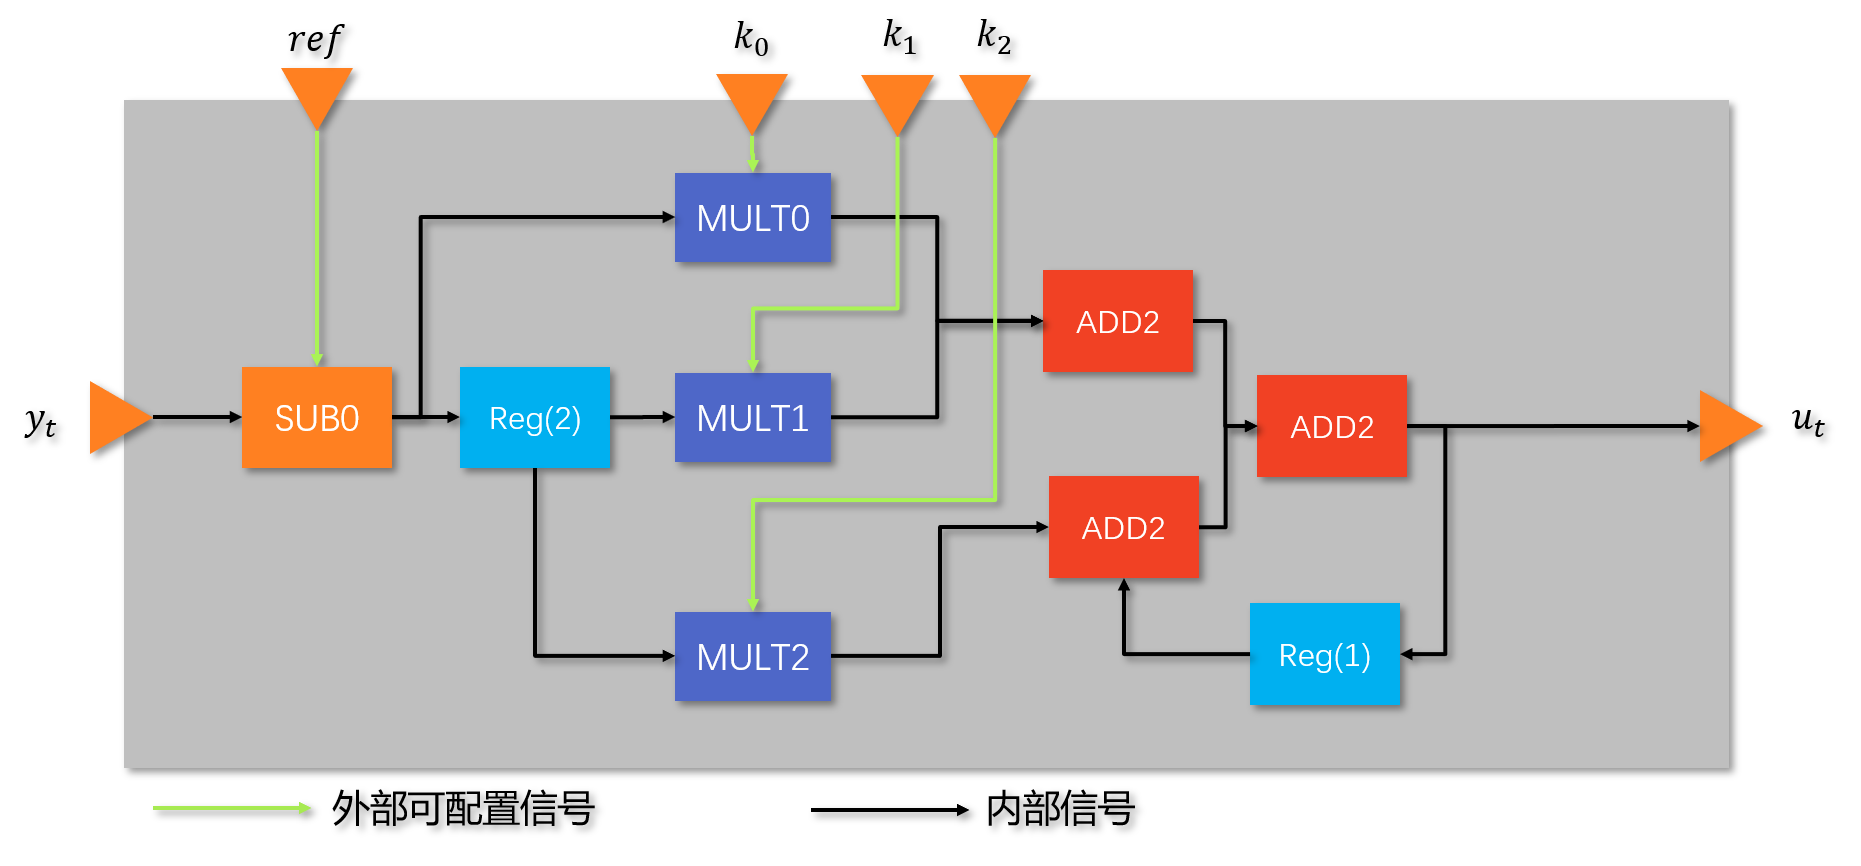
\includegraphics[width=1.0\linewidth]{rtmq/digital_pid_structure_16bits_s}
\end{figure}

离散化后的PID表达式为:
\begin{align}
    u(n)=k_p e(n)+k_i\sum_{j=-}^{n}e(j)+k_d[e(n)-e(n-1)]\\
    u(n-1)=k_p e(n-1)+k_i \sum_{j=0}^{n-1}e(j)+k_d [e(n-1)-e(n-2)]
\end{align}

由上面两式可以导出:

\begin{align}
    \Delta u(n)=&u(n)-u(n-1)\\
    =&k_0 e(n)+k_1 e(n-1)+k_2 e(n-2)
\end{align}

其中$k_0=k_p+k_i+k_d,\ k_1=-k_p-2k_d,\ k_2=k_d$,这个式子被称为PID的增量算法。采用这种形式的好处是避免了计算PID原始表达式中的无限积分项。在这种增量式的方式下,PID的控制输出可以表达为:
\begin{align}
    u(n)=u(n-1)+\Delta u(n)=u(n-1)+k_0 e(n)+k_1 e(n-1)+k_2 e(n-2)\label{eq:increment_pid}
\end{align}

按照上述式\eqref{eq:increment_pid}表示的增量式算法,数字PID实现的结构示意图如图\ref{fig:digital_pid_structure_16bits_s}所示。接口主要有参考$ref$、参数$k_0, k_1, k_2$等可配置输入,反馈信号$y_t$等系统回路输入,以及$u_t$等系统控制输出。用到的器件包括加法器/减法器(图示中红、橙色模块)、乘法器(图示中蓝色模块)、寄存器(图示中靛色模块)。

\subsection[数字PID的FPGA实现]{数字PID的硬件实现}

% 增量式PID最终在FPGA中实现的结构图如图\ref{fig:digital_pid_structure_16bits}所示。

根据图\ref{fig:digital_pid_structure_16bits_s}所示的结构,可以在FPGA中实现硬件的PID。其中涉及到的数字加法器、数字乘法器在第\ref{section:carray_lookahead_adder}节和第\ref{section:booth_multiplier}节中已经有过介绍。对于高速时序电路,在开发过程中需要注意流水线的设置和对齐,最终的实现硬件框图如图\ref{fig:digital_pid_structure_16bits}所示。
\begin{figure}
    \centering
    \caption[16位数字滤波器FPGA实现结构图]{16位数字滤波器FPGA实现结构图\label{fig:digital_pid_structure_16bits}}
    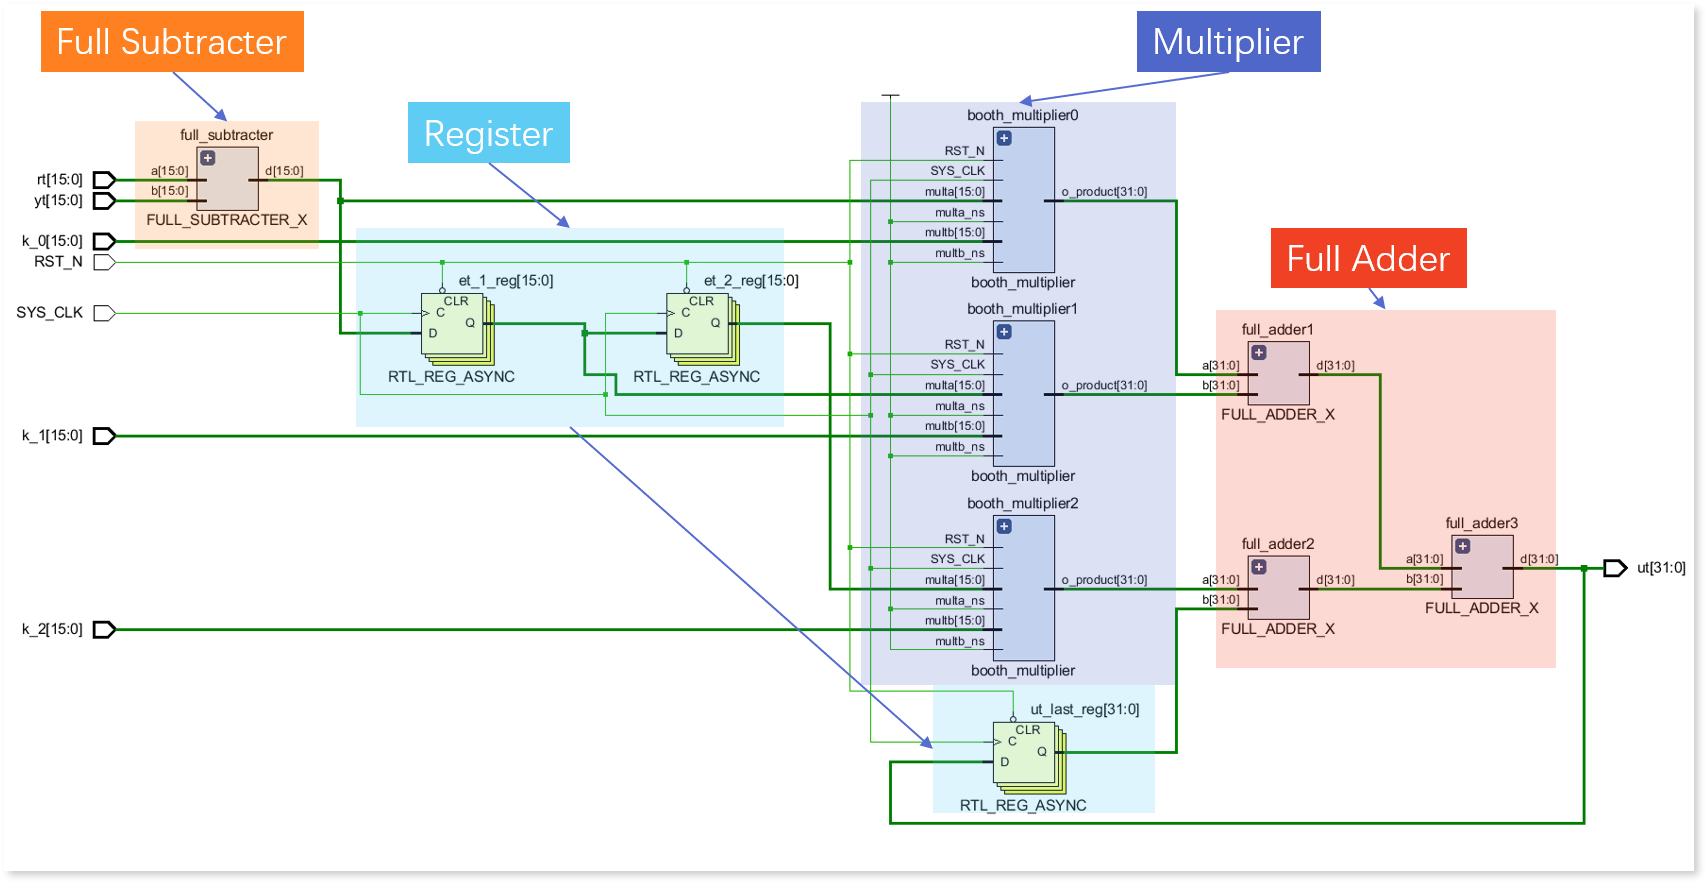
\includegraphics[width=1.0\linewidth]{rtmq/digital_pid_structure_16bits}
\end{figure}

整个PID控制器使用了一个减法器、三个加法器、三个乘法器和若干寄存器。图\ref{fig:digital_pid_structure_16bits}是一个16位输入的数字PID,它的输出是32位的,该实例模块总共包含9级流水线,工作频率可达200MHz以上。对更低或者更高位数的数字PID控制器,可以通过替换相应位数的加减运算和乘法模块,并调整相应的寄存器位宽来方便地得到。




\newpage
\section[基于FPGA的通用数字滤波器]{基于FPGA的通用数字滤波器\label{section:digital_iir}}
\textcolor{red}{
1. 介绍数字滤波器功能、种类、基本原理,比如有限冲激响应滤波器、无限冲激响应滤波器等等;}

\textcolor{red}{
2. 介绍数字通用滤波器功能、逻辑图、Vivado中的实现、优势;}

IIR滤波器结构如图\ref{fig:iir_filter_s}所示。
\begin{figure}
    \centering
    \caption[IIR滤波器结构框图]{IIR滤波器结构框图\label{fig:iir_filter_s}}
    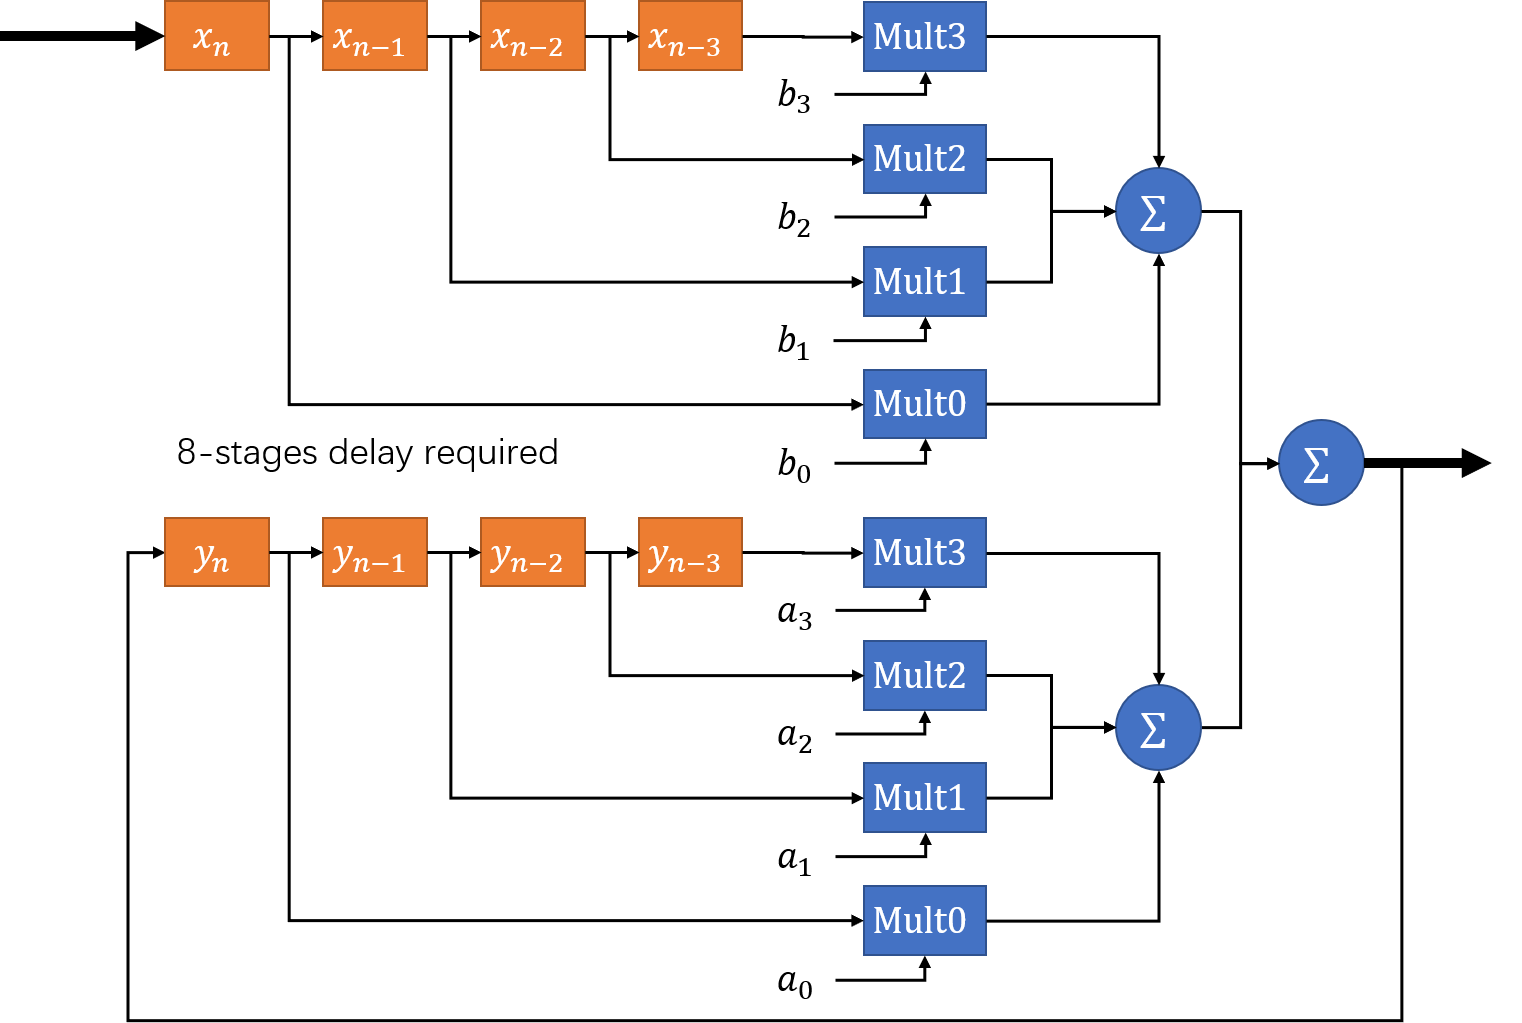
\includegraphics[width=1.0\linewidth]{rtmq/iir_filter_s}
\end{figure}




% !TeX root = ../sustechthesis-example.tex

\chapter[螺线管谐振腔]{螺线管谐振腔\label{section:helical}}
% \textcolor{red}{
% 这部分将对之前谐振腔的研究进行整理和总结...
% }
\section[离子阱系统中的螺线管谐振腔]{离子阱系统中的螺线管谐振腔}

如前面在第\ref{section:ion_trap_quantum_computation_system}章中所介绍的,Paul阱是离子阱量子计算实验平台上普遍使用的阱,它也是一类具有代表性的离子阱,利用交替电流(Alternating-Current, AC)电场来动态囚禁带电原子或粒子。上述交流场的频率总是落在射频(RF)范围内,而相应的电压可以达到几百伏。通常,将这种高压射频信号直接应用于Paul阱的电极是具有挑战性的,因为阱本身可以被视为纯电容器件;因此,信号发生器和阱之间的阻抗失配使得功率注入效率低下。

解决上述困难的标准方法是使用螺线管谐振腔来作为信号发生器和离子阱之间的“桥梁”。一个设计合适的螺线管谐振腔既能够实现阻抗匹配的要求也能够放大施加到阱电极上的电场。同时,它还充当带通滤波器来阻断潜在的电子噪声。因此,螺线管谐振腔是离子陷阱系统中最关键的角色之一。

对于螺线管谐振腔,它通常具有两个基本特性,即谐振频率$f_0$和品质因子$Q$。它们的值主要由谐振腔本身的几何设计决定,如图\ref{fig:helical_structure_2d}所示。
设计螺线管谐振腔的主要目标是找到合适的几何参数,使得谐振频率$f_0$与期望值相匹配,并最大化品质因子$Q$。设计谐振器的一种方法是由其简化的LC电路模型指导,并利用经验公式从几何参数估计相应的电容、电感和电阻。
然而,为了使用经验公式,某些几何参数之间的比率仅限于给定的区间,而且估计的$f_0$和$Q$总是偏离实际值。
近来,一种基于商业软件的有限元(Finite Element, FE)仿真的设计方法开始被广泛使用。与经验估计方法相比,使用FE方法模拟谐振腔在属性评估方面提供了更高的准确性,在几何设计方面提供了更大的灵活性。

\begin{figure}
    \centering
    \caption[谐振腔结构平面示意图]{谐振腔结构平面示意图。$H$:耦合线圈底部到主线圈底部的距离;$B$:屏蔽壳侧壁长度;$D$:屏蔽壳内筒直径;$\tau$:主线圈螺距;$d_0$:主线圈线粗;$d$:主线圈直径;$b$:主线圈总长度;$l_{out}$:输出线长度;$D_1$:输出口内直径。\label{fig:helical_structure_2d}}
    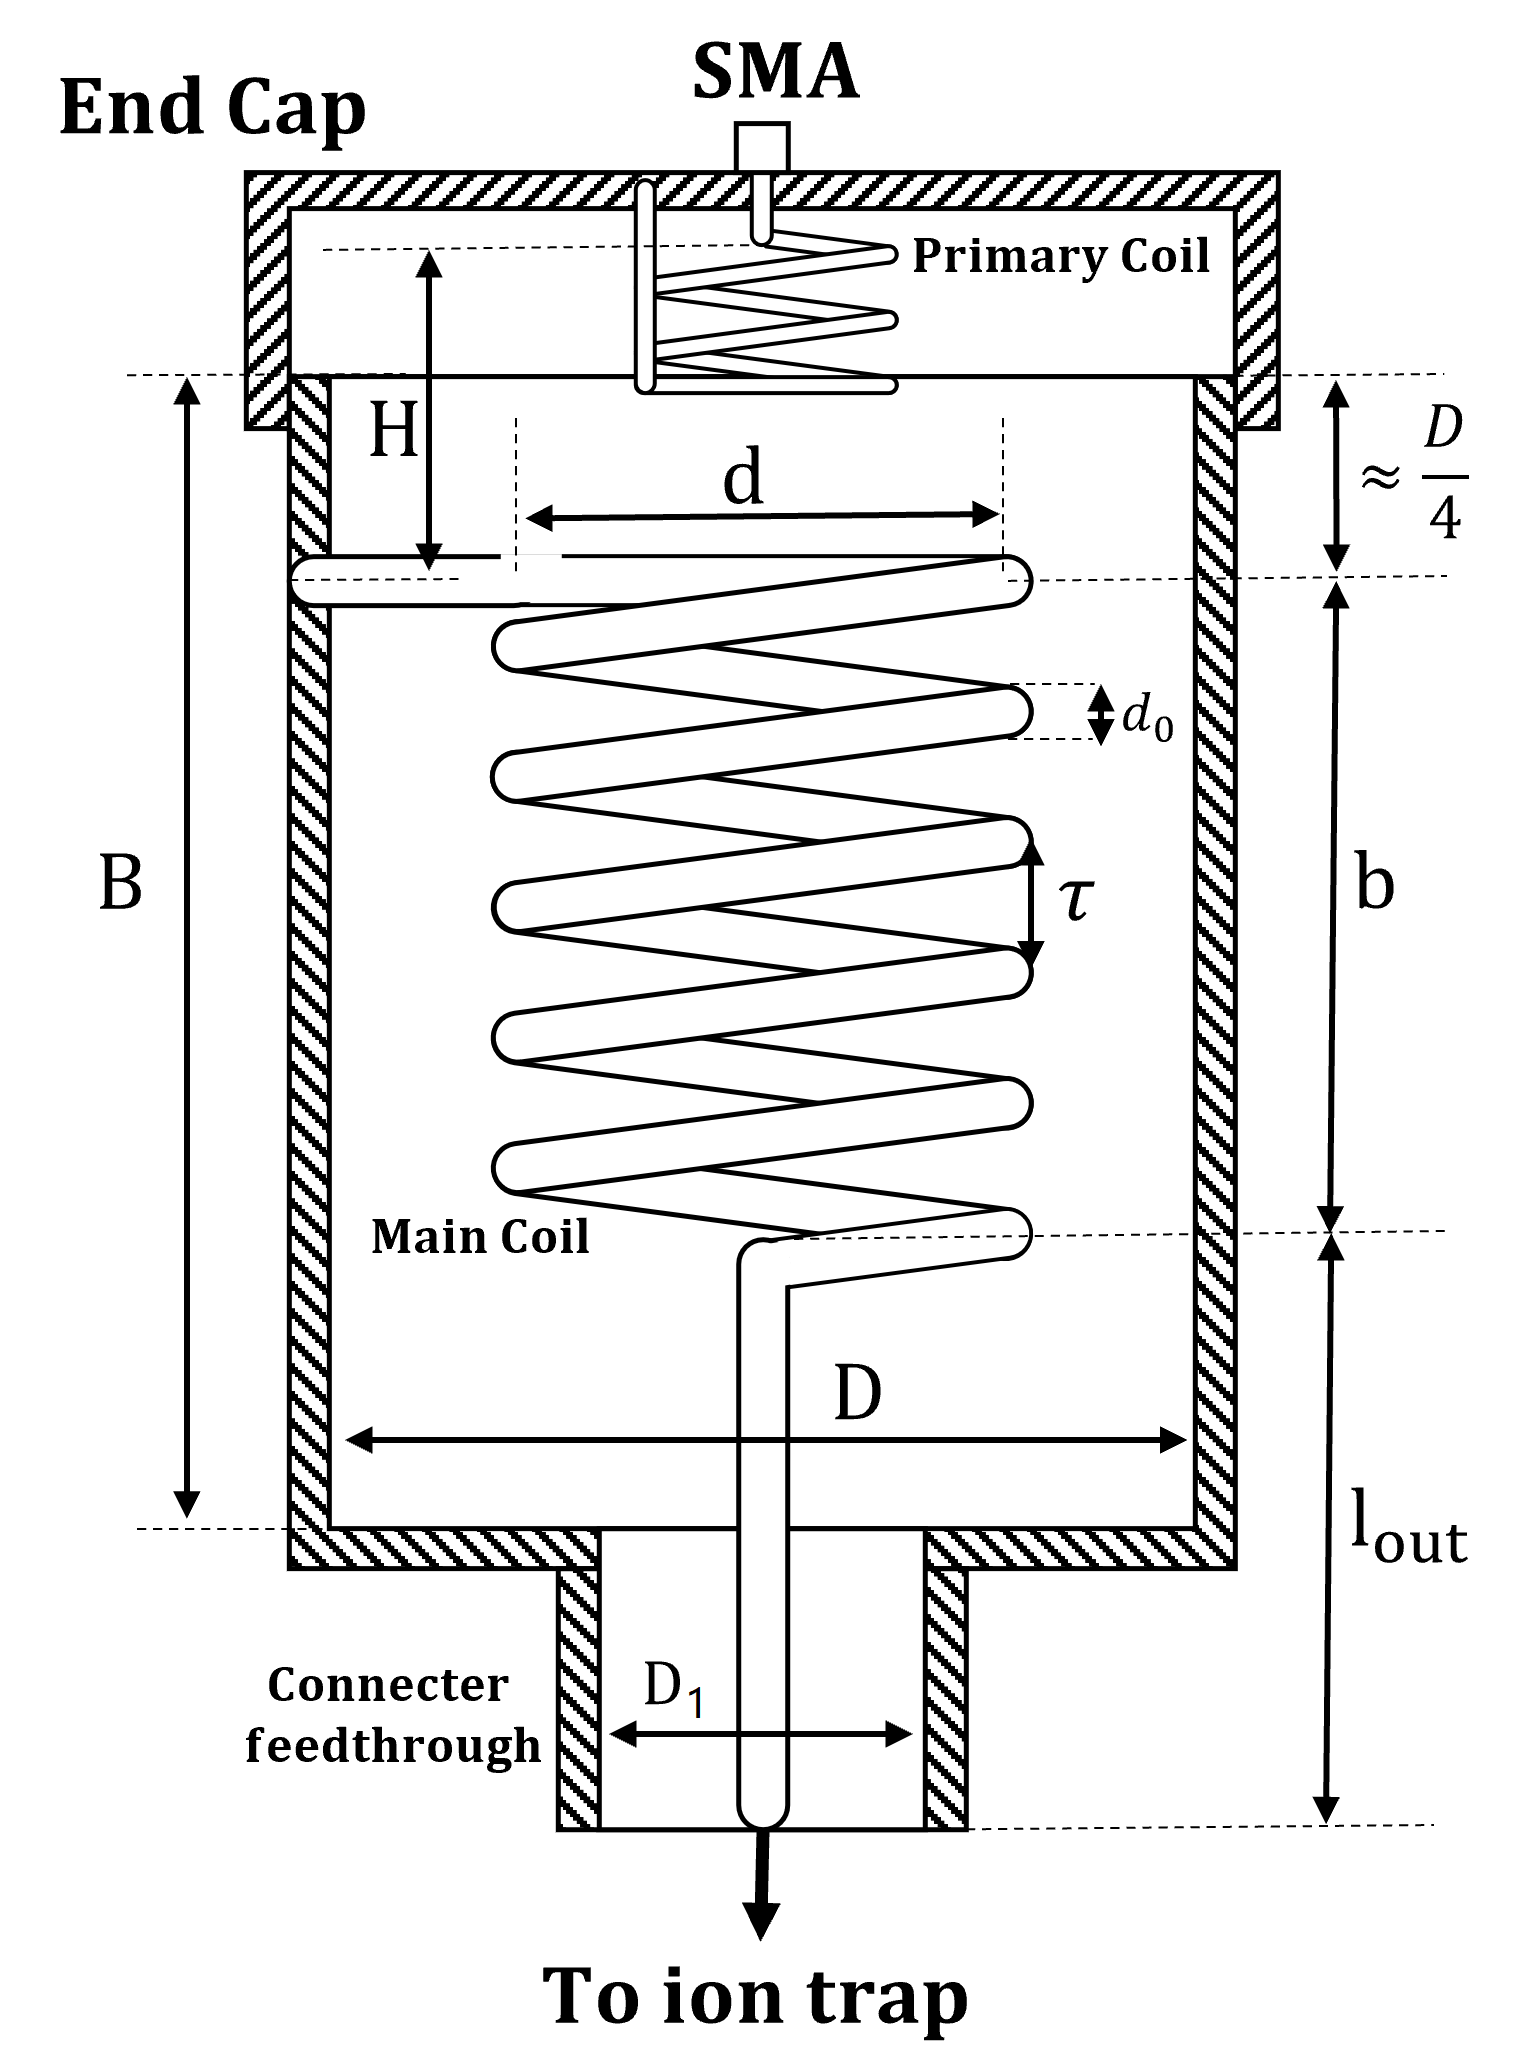
\includegraphics[width=0.5\linewidth]{helical/helical_structure_2d}
\end{figure}

\section[螺线管谐振腔的仿真]{螺线管谐振腔的仿真}

常用的商业化FE仿真工具有ANSYS HFSS、Comsol等,接下来的仿真中我们采用的ANSYS HFSS来研究影响谐振腔$f_0$和$Q$值的各种因素。在HFSS中,有两种方法可以分析3D结构,本征模模式(Eigen-mode)和驱动模式(Driven-mode)。
本征模模式通过分析计算电磁场模式,直接给出谐振频率$f_0$和品质因子$Q$的结果;而驱动模式是通过设置输入和输出微波端口,分析和计算\emph{散射参数(Scattering Parameter, SP)},与实验更具可比性。
这两种模式都可以用来模拟螺线管谐振腔,但本征模法更常用于谐振器设计,驱动模态在一般仿真中更为频繁。因为驱动模式得到的结果可以直接与实际实验结果做比对,在接下来的仿真研究中我们默认使用这种方法来进行仿真(特别说明的情况除外)。
请注意,由于阻抗匹配网络损耗\cite[]{Gandolfi_Niedermayr_Kumph_Brownnutt_Blatt_2012},驱动模态中品质因子$Q$的结果大约是本征模结果的一半。

我们在仿真软件中构建了与实际谐振器相同的一个3D模型。模型结构示意图如图\ref{fig:helical_structure_2d}所示,HFSS中建立的3D模型视图如图\ref{fig:helical_HFSS_3d}所示。
在这个3D模型中,除了主线圈和铜壳结构外,它还包括耦合线圈、输出导线$l_{out}$和连接器馈通结构,3D模型的所有实体结构均为紫铜材料。
主线圈与铜屏蔽壳侧壁接触(gnd);在耦合线圈和主线圈设置两个集总端口,耦合线圈作为输入端口,主线圈作为输出端口,如图\ref{fig:helical_HFSS_3d}中黄色的圆片所示。通过调整耦合线圈到主线圈的距离可以实现阻抗匹配,阻抗匹配的目标是使得S参数反射最小,仿真中采用的标准是$S_{11}<-40$dB。仿真结果的后处理与实际实验完全相同,中心频率$f_0$和$Q$因子可以从$S$参数导出。

\begin{figure}
    \centering
    \caption[HFSS中建立的3D模型图]{HFSS中建立的3D模型图。黄色圆片表示微波输入和输出端口;橙色部分表示耦合线圈和主线圈,一般采用紫铜材质制作;绿色部分是屏蔽外筒,一般采用紫铜或者黄铜制作。\label{fig:helical_HFSS_3d}}
    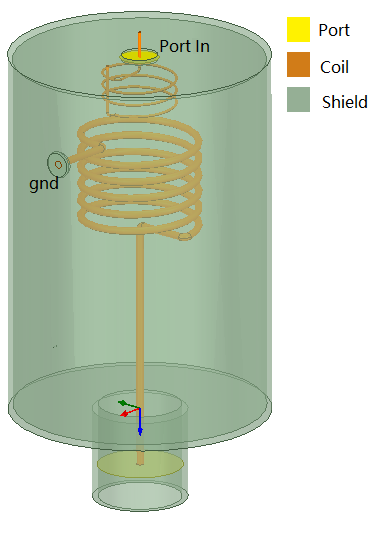
\includegraphics[width=0.4\linewidth]{helical/helical_HFSS_3d}
\end{figure}

离子阱实验中的谐振频率通常在$10-100$MHz之间,主线圈的典型直径和螺距间距分别为$50-60 $mm和$5-8$mm。为了测试HFSS模拟和实验之间的一致性,我们选择了三组几何设置,如表\ref{tb:helical_simulation_parameters}所示。
在每个组中,谐振器具有相似的谐振中心频率,但线圈直径和绕组间距不同,即$30$MHz、$50$MHz、$75$MHz组。
除了正常参数外,我们故意选择一个更大的参数范围,接近线圈直径和绕组间距的极限,比如线圈直径在$30-80$mm之间(与屏蔽直径$D=103$mm相比);绕组间距在$4mm$到$ 18$mm之间(与导线直径为$d0 = 3$mm相比)。
关于其它参数,参数$d=48$mm$/\tau = 7$mm的初始轮数$N = 5.734$,屏蔽外壳的高度$ B = 136$mm。螺旋谐振器由网络分析仪Keysight E5063A进行了实验测试。实验测试方案和螺旋谐振器的照片如图\ref{fig:helical_experiment_test}所示。
\begin{table}
    \centering
    \caption[仿真的谐振腔参数设置]{仿真的谐振腔参数设置\label{tb:helical_simulation_parameters}}
    \begin{tabular}{lccccccc}
        %Left\footnote{Note a.}&Centered\footnote{Note b.}&Right\\
        \toprule
        $\#$ & groups & d & $\tau$ & $f_{HFSS}$ & $Q_{HFSS}$ & f$_{exp}$ & $Q_{exp}$ \\
        \midrule

        1 & \multirow{5}*{30MHz} 	& 40 & 4  & 32.4062 & 565 & 31.7472 & 513   \\
        2 & 						& 80 & 4  & 25.2663 & 346 & 24.8038 & 207   \\
        3 & 						& 60 & 5  & 28.4732 & 639 & 28.3904 & 587   \\
        4 & 						& 50 & 6  & 30.2228 & 650 & 30.6030 & 599   \\
        5 & 						& 80 & 10 & 27.1943 & 354 & 27.6059 & 317   \\
        \midrule
        6 & 50MHz 					& 48 & 5  & 49.878739 & 708 & 49.2687 & 631   \\
        \midrule
        7 & \multirow{5}{*}{75MHz} 	& 30 & 4  & 76.4602 & 595 & 76.2748 & 542   \\
        8 & 						& 80 & 4  & 61.2866 & 453 & 60.7942 & 389   \\
        9 & 						& 48 & 7  & 74.9382 & 802 & 75.2466 & 708   \\
        10 & 						& 40 & 14 & 88.4308 & 686 & 88.8163 & 571   \\
        11 & 						& 80 & 18 & 77.9517 & 469 & 78.4634 & 377   \\
        \bottomrule
    \end{tabular}
\end{table}


\begin{figure}
    \centering
    \caption[实际实验的测量方式示意图]{实际实验的测量方式示意图\label{fig:helical_experiment_test}}
    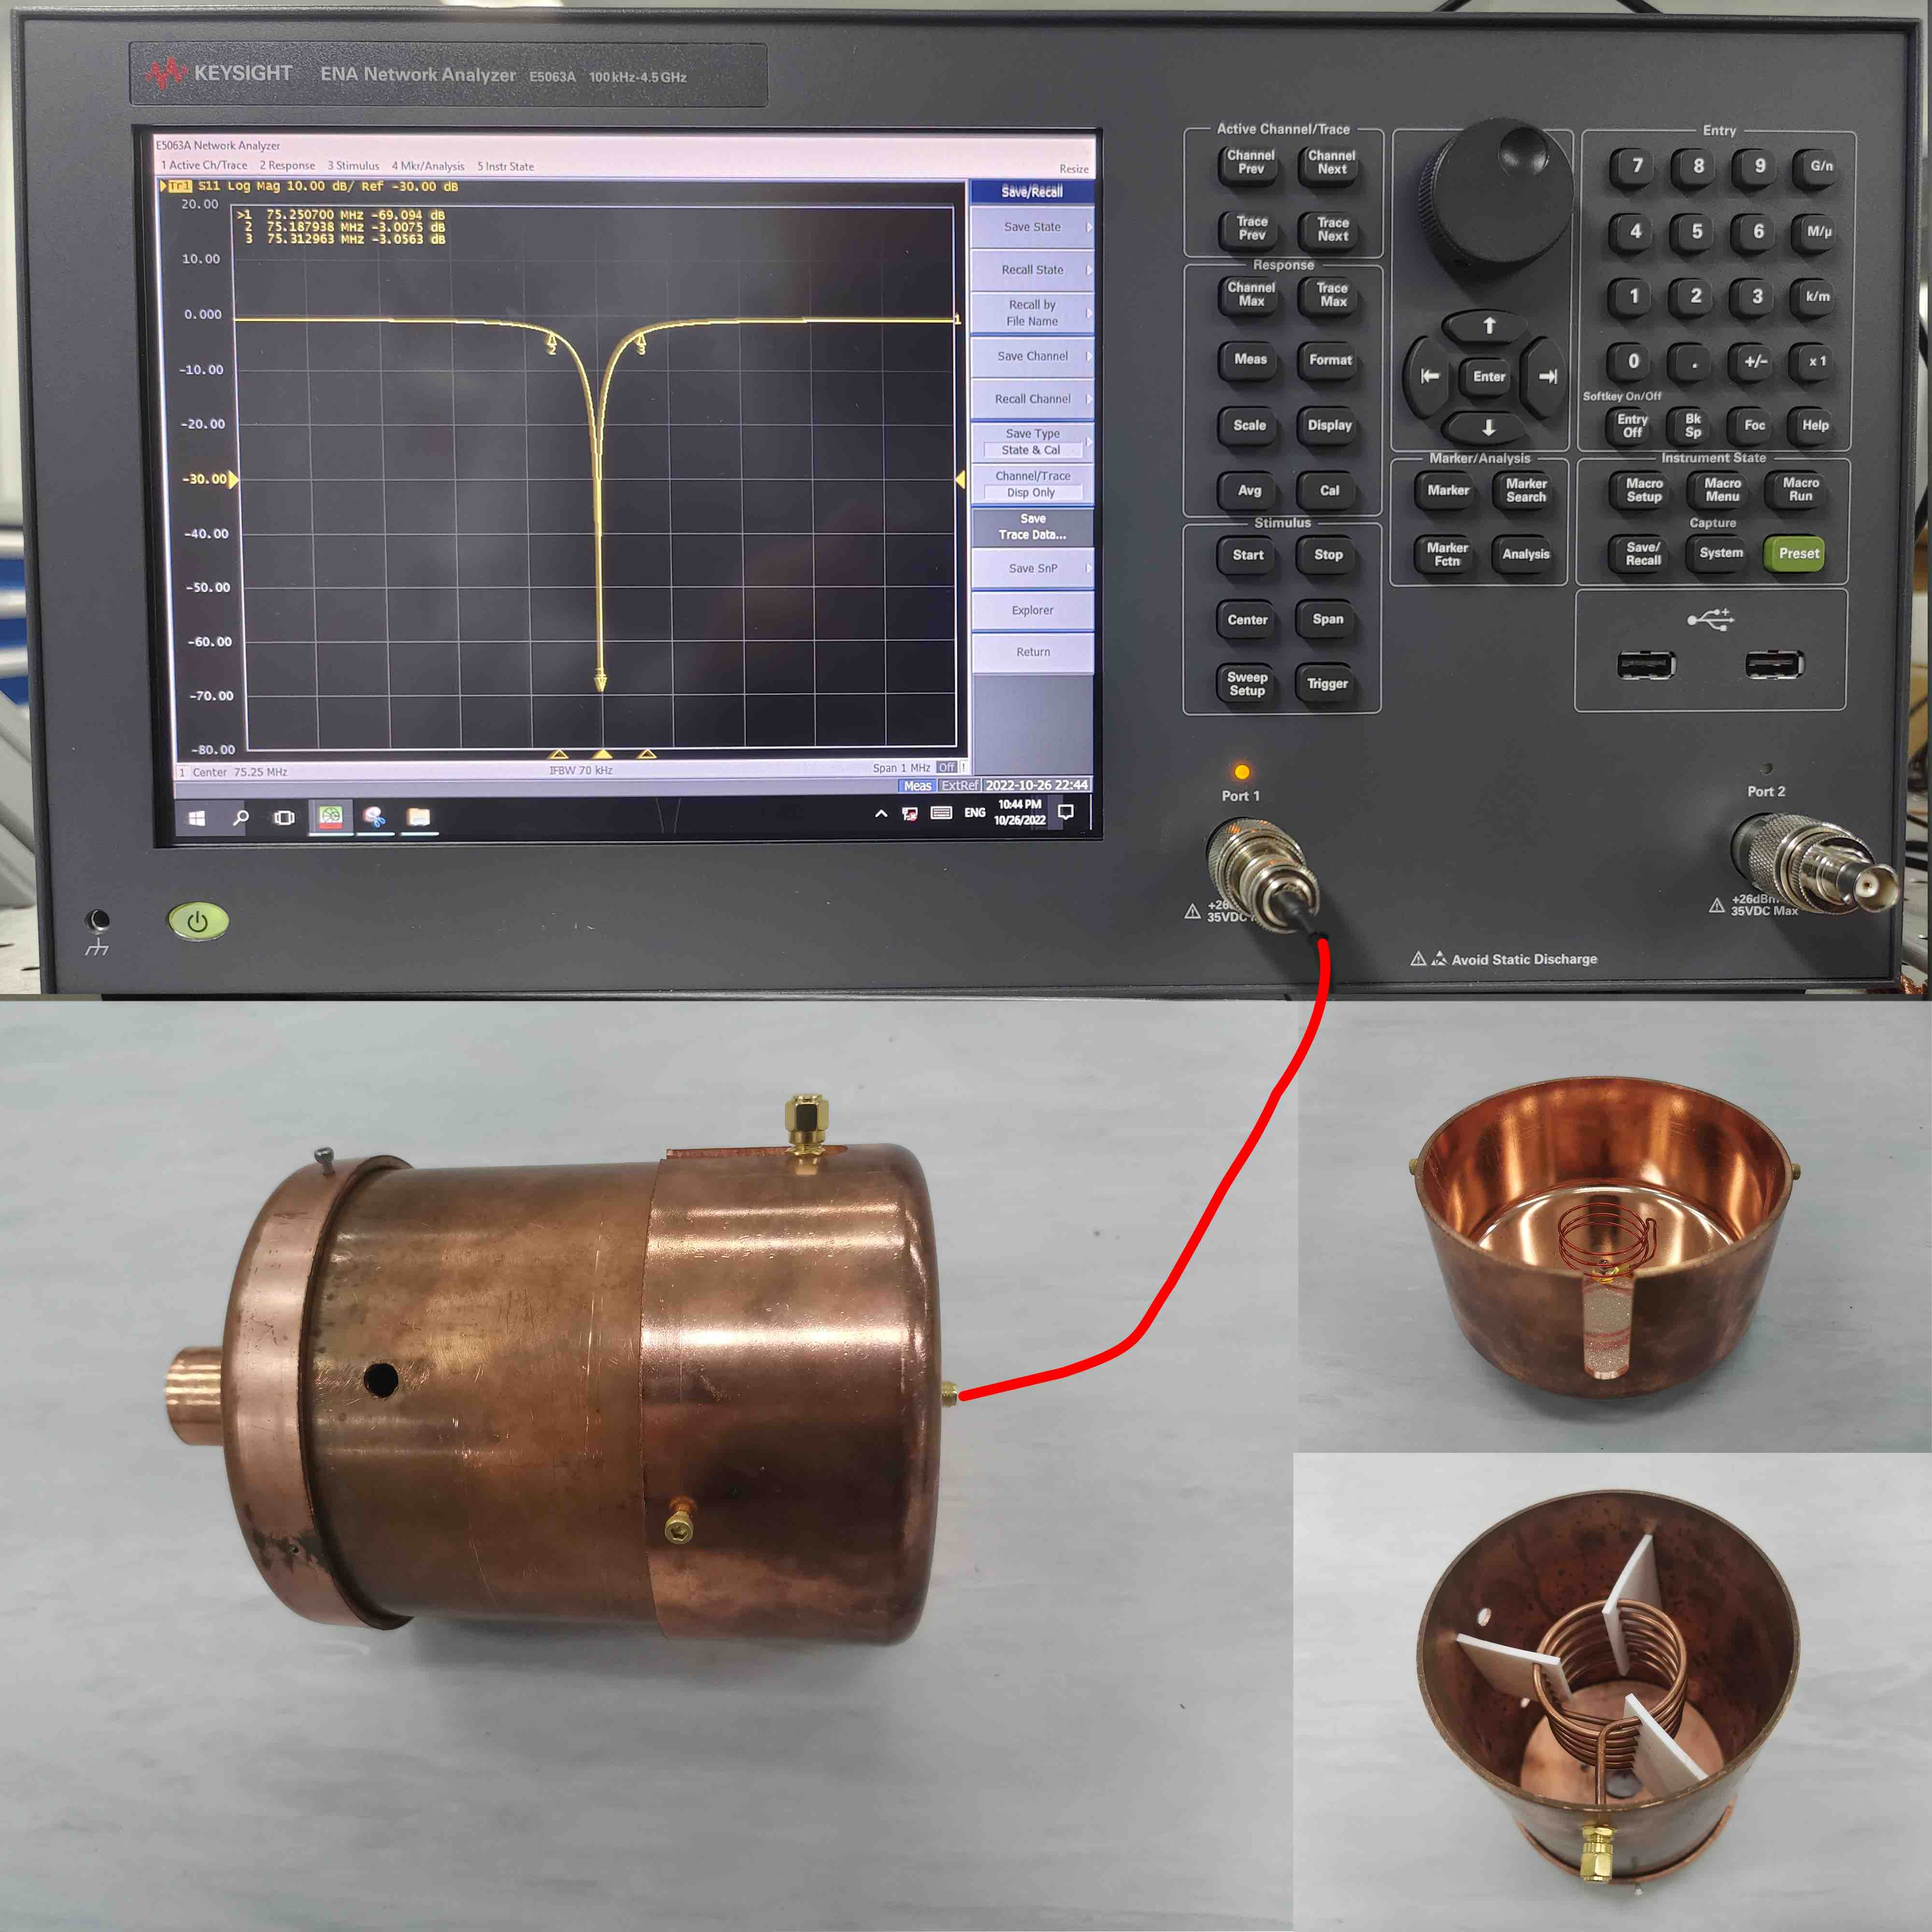
\includegraphics[width=1.0\linewidth]{helical/helical_experiment_test}
\end{figure}

我们选择在表\ref{tb:helical_simulation_parameters}中的2、6、9三行设置作为示例来比较HFSS模拟和实验的结果,散射参数$S_{11}$的对比结果如图\ref{fig:helical_compares}所示(中心频率平移到相互重合,以便清楚地显示$S_{11}$的差异)。结果中的差异$\Delta f(Q)=f(Q)_{exp}-f(Q)_{HFSS}$。实验测试的频率$f_0$和品质因子$Q$结果和误差棒如图\ref{fig:helical_compares_f_q}所示。误差条非常小,几乎不可见。频率的最大差异约为$0.7$MHz。除了一个设置的$Q$因子差为$-122$,其他$Q$因子的差异约为或小于$60$。相对较大的$Q$偏差的原因可能是由于频率和电阻影响。
频率的大小受到电感和电容的影响,电感和电容的具体值由谐振腔的几何结构和材料决定。
电阻受材料和加工过程的影响,例如焊点电阻、金属表面氧化等。此外,我们模拟了我们之前使用的几种螺旋设计,并与实验记录相比,频率差异小于$1$MHz,$Q$差异小于 $50$。

以上结果表明,仿真方法都能较好地预测实验结果。这验证了HFSS商业软件是帮助设计和预测螺旋谐振器行为的绝佳工具,为谐振腔的研究提供了极大的方便。

\begin{figure}
    \centering
    \caption[谐振腔仿真与实验散射参数结果对比]{谐振腔仿真与实验散射参数$S_{11}$结果对比。其中红色实线为HFSS仿真结果,蓝色实线为实验测得的结果。横坐标为频率(单位MHz),纵坐标为幅度(单位dB)。\label{fig:helical_compares}}
    \subcaptionbox[50MHz]{50MHz}{
        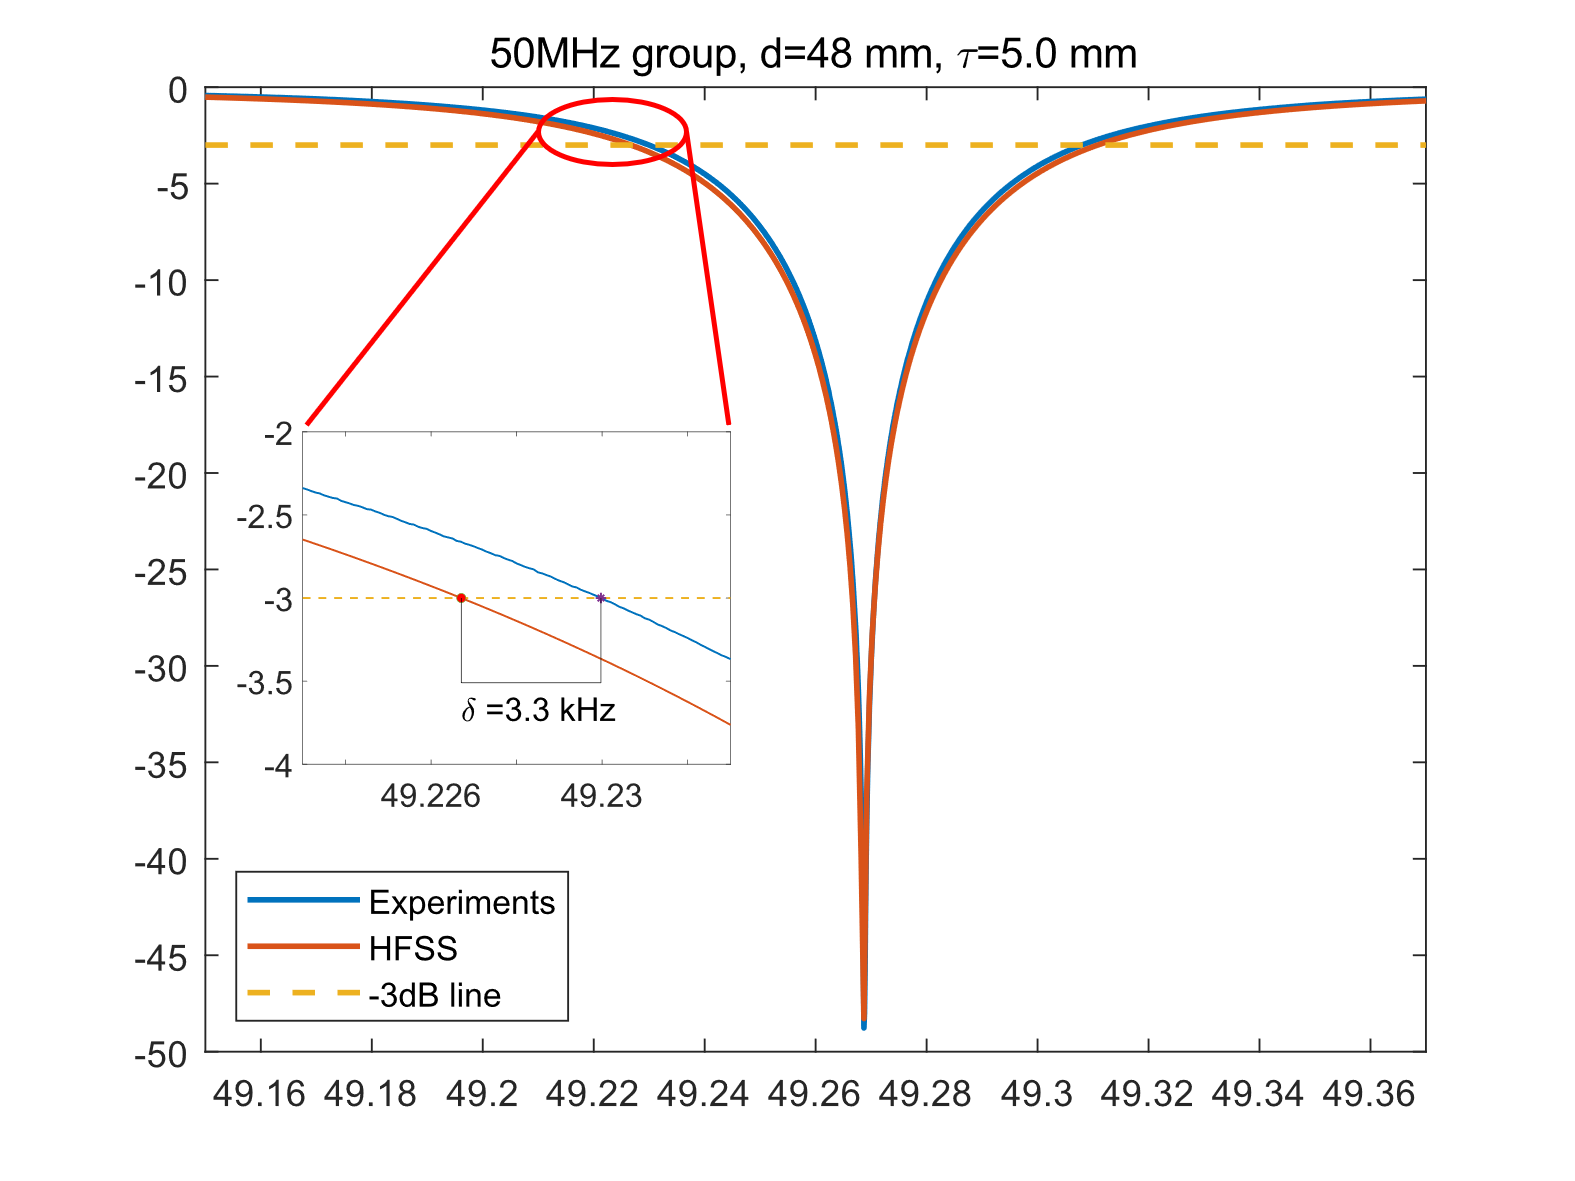
\includegraphics[width=1.0\linewidth]{helical/helical_50MHz_final}
    }
    \subcaptionbox[30MHz]{30MHz}{
        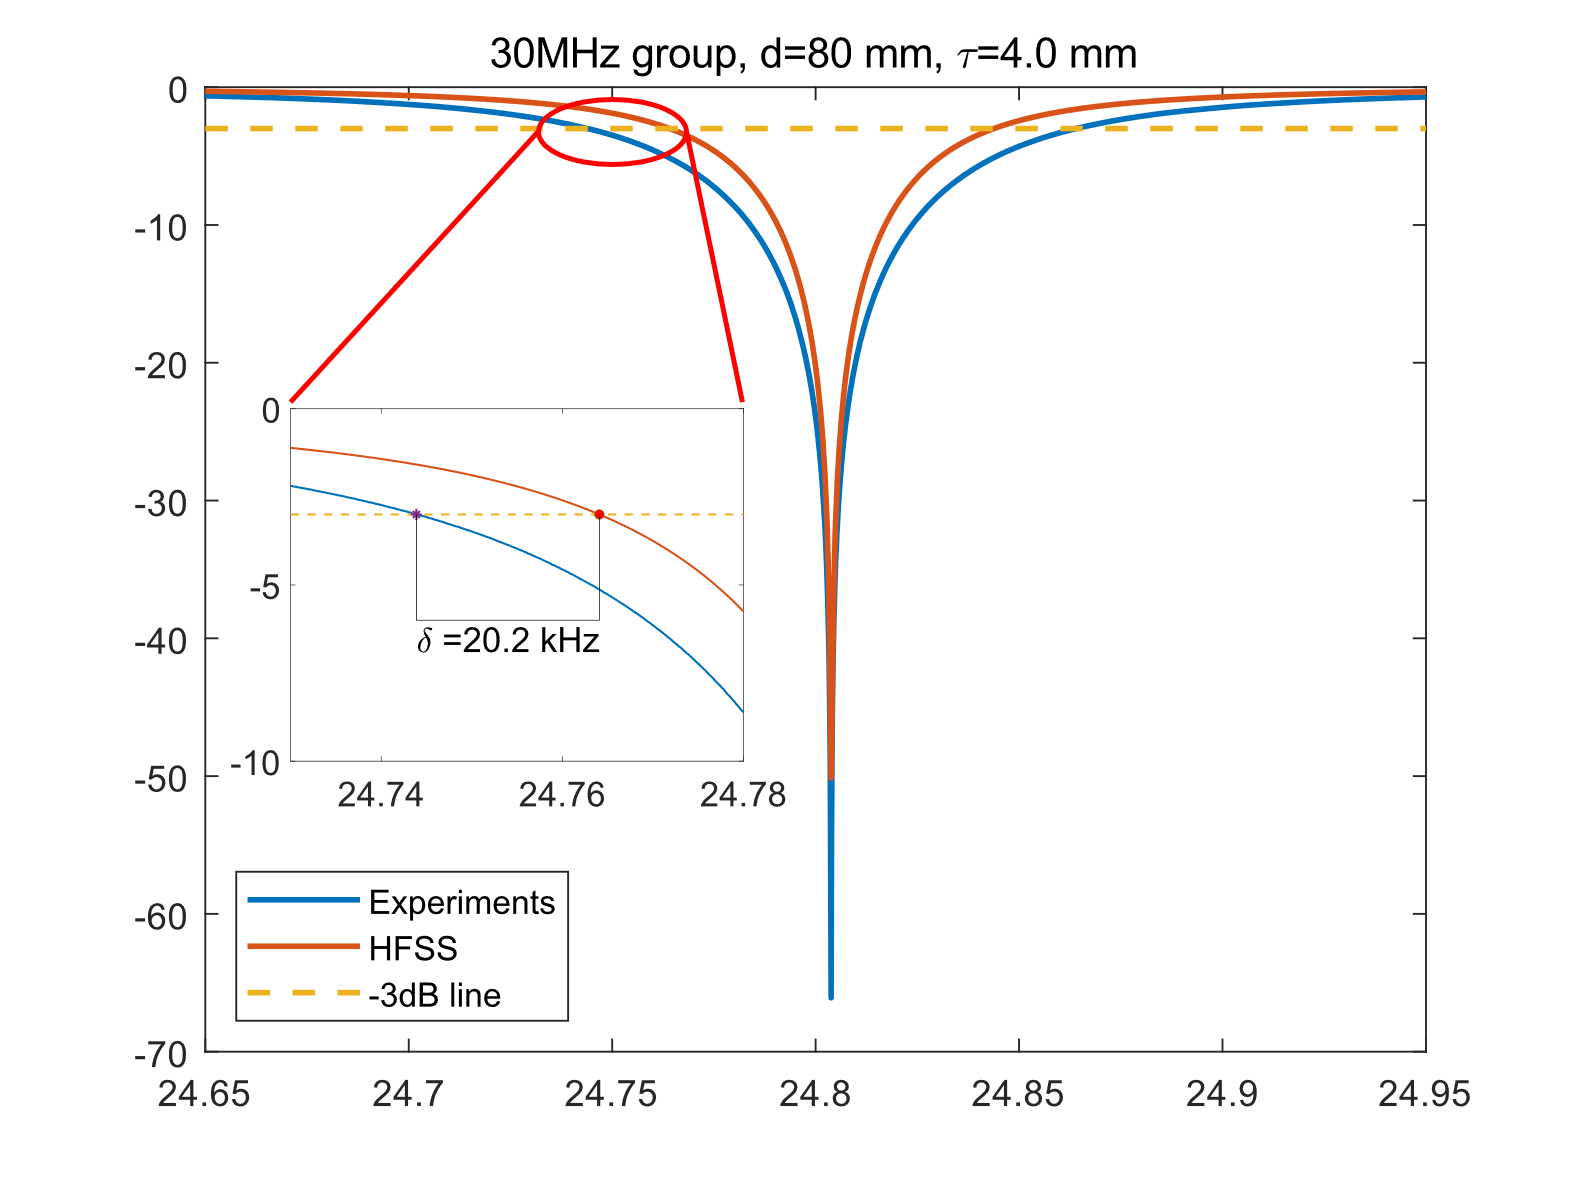
\includegraphics[width=0.46\linewidth]{helical/helical_30MHz_final}
    }
    \subcaptionbox[75MHz]{75MHz}{
        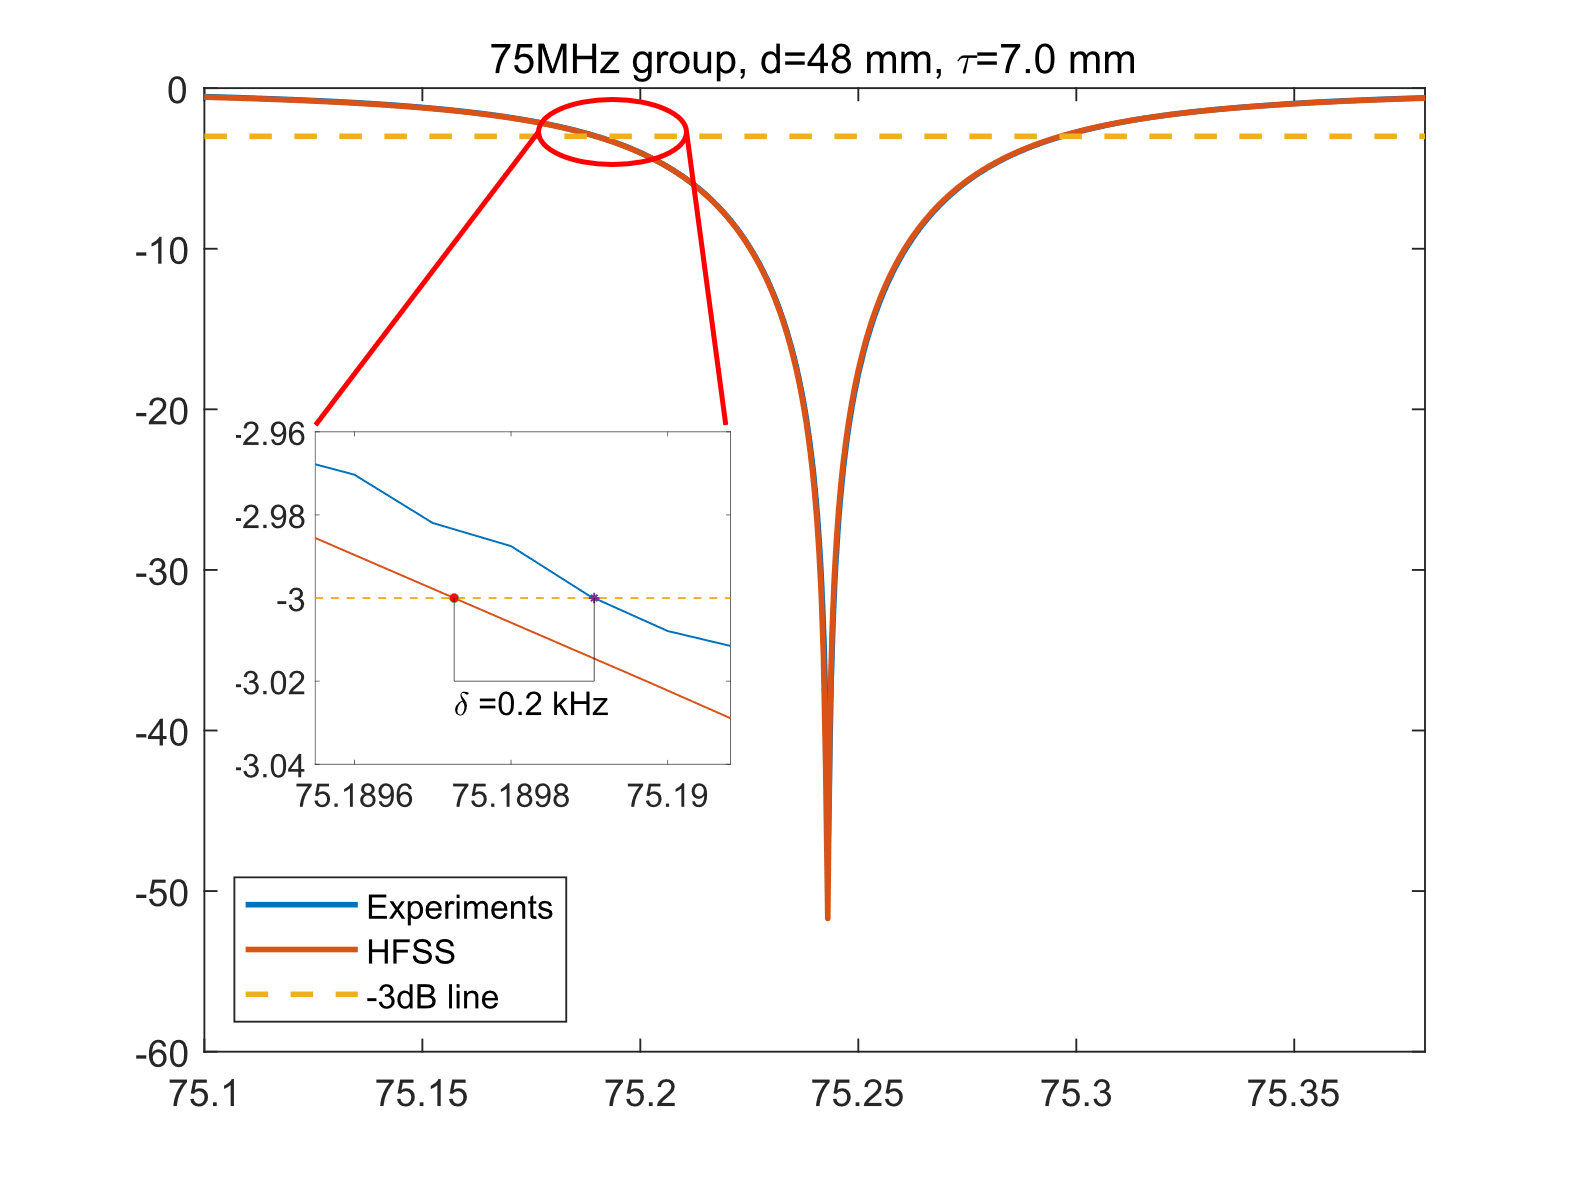
\includegraphics[width=0.46\linewidth]{helical/helical_75MHz_final}
    }
\end{figure}


\begin{figure}
    \centering
    \caption[谐振腔仿真与实验频率和Q结果对比]{谐振腔仿真与实验频率和Q结果对比。横坐标为表中对应的序号数,(a)纵坐标为实验与仿真预测的频率结果偏差$\Delta f$(单位MHz),(b)纵坐标为实验与仿真预测的Q值结果偏差$\Delta Q$(单位1)。\label{fig:helical_compares_f_q}}
    \subcaptionbox[谐振腔仿真与实验频率结果对比]{谐振腔仿真与实验频率结果对比}{
        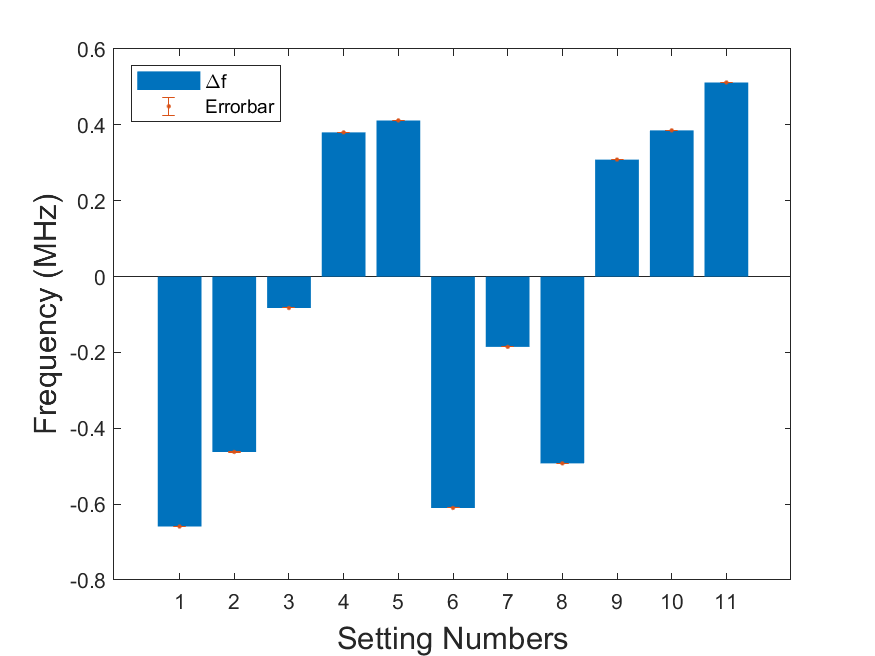
\includegraphics[width=0.48\linewidth]{helical/helical_delta_f}
    }
    \subcaptionbox[谐振腔仿真与实验Q结果对比]{谐振腔仿真与实验Q结果对比}{
        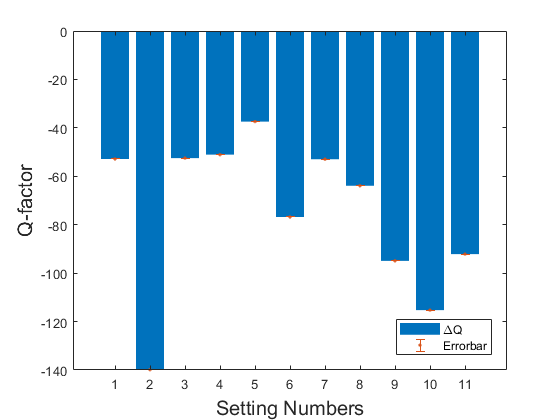
\includegraphics[width=0.48\linewidth]{helical/helical_delta_Q}
    }
\end{figure}

\section[几何参数对频率和Q的影响]{几何维度对频率和Q的影响}

在离子阱的应用中,螺线管谐振腔最重要的性能是谐振频率和Q因子,具有特定谐振频率和最高$Q$因子的谐振腔是最理想的\cite[]{Siverns_Simkins_Weidt_Hensinger_2012}。
谐振频率和Q可以由以下包含集总参数电感$L$、电容$C$和电阻$R$的公式表达:
\begin{align}
    f&=\frac{1}{2\pi\sqrt{LC}} \label{eq:helical_f_equation}\\
	Q&=\frac{\omega L}{R}=\frac{1}{R}\sqrt{\frac{L}{C}} \label{eq:helical_Q_equation}
\end{align}

对于特定的材料,几何物理参数完全决定了设备的所有特性和等效的集总电路参数。进一步地,频率主要取决于电感和电容两者的比值$L/C$,从几何角度看就是取决于谐振腔主线圈的直径、螺距以及总线长等;在此基础上,$Q$除了跟$L/C$有关外,还与电阻有关。
在之前的研究中,大多数研究人员将线圈直径、绕组间距和主线圈数视为非独立参数\cite[]{Siverns_Simkins_Weidt_Hensinger_2012,Macalpine_Schildknecht_1959}。
然而,在我们的模拟中,我们发现如果主线圈的总长度是固定的,谐振频率将比总导线长度变化小得多,结果如图\ref{fig:helical_fixedwirelength}所示。
这使得谐振频率的控制更容易。一项研究\cite[]{Nandi_Sikdar_Das_Ray_2022}也指出了这种类似的现象,它给出了谐振频率与主线圈长度之间的关系。螺线管谐振腔基本上与四分之一波长谐振器相同。
\begin{figure}
    \centering
    \caption[固定线长下改变主线圈参数的频率$f_0$变化]{固定线长下改变主线圈参数的频率$f_0$变化。(a)横坐标为主线圈直径$d$(单位mm),(b)主线圈螺距$\tau$(单位mm);纵坐标为频率$F$(单位MHz)。\label{fig:helical_fixedwirelength}}
    \subcaptionbox[改变主线圈直径参数]{改变主线圈直径参数}{
        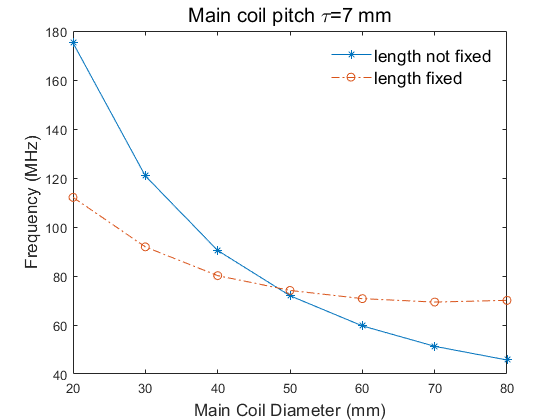
\includegraphics[width=0.48\linewidth]{helical/helical_fixedwirelength_1}
    }
    \subcaptionbox[改变主线圈螺距参数]{改变主线圈螺距参数}{
        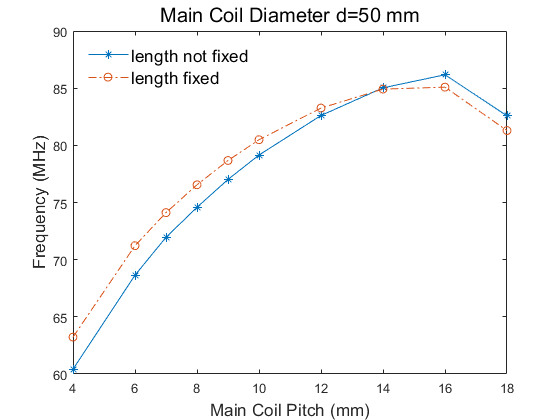
\includegraphics[width=0.48\linewidth]{helical/helical_fixedwirelength_2}
    }
\end{figure}

在我们的模拟中,主要线圈几何形状设置了两个限制,即固定的总导线长度$l_{total}$和固定的总导线高度$h$:
\begin{align}
    l_{total}&=N\sqrt{(\pi d)^2+\tau^2}+l_{out} \label{eq:helical_fixed_constraints_1}\\
	h&=N\tau+l_{out} \label{eq:helical_fixed_constraints_2}
\end{align}

因此,频率在$d=20 $mm到$d=80 $mm时平均变化约为$0.701$MHz/mm;虽然绕组间距效应不那么明显,但频率在$\tau=4 $mm到$\tau=118 $mm时平均变化约为$1.29$MHz/mm。这种现象有助于分离几何效应和频率变化之间$ Q $因子改进的原因。接下来的几节将在这些预设下,研究几个几何参数的效应来设计所需的频率$f_0$和$Q$因子。
\subsection[主线圈几何参数的影响]{主线圈几何参数的影响}

为了研究对谐振频率$f_0$和$Q$因子的几何效应,基于表\ref{tb:helical_simulation_parameters}中第9行的参数,对几组主线圈参数进行设置和模拟。
主线圈的直径和间距设置为双参数扫描;直径从$30-80$mm,步长为$10$mm;螺距设置为$4-18$mm,步长为$2$mm。
这些模拟的结果给出了一个谐振频率$f_0$和$Q$因子的几何效应图,将其绘制为等高线图,如图\ref{fig:helical_contour}所示。左上角的白色三角形是参数禁止区,因为主线圈参数不满足约束公式\eqref{eq:helical_fixed_constraints_1}和\eqref{eq:helical_fixed_constraints_2}。
使用一组确定的参数($d$和$\tau$),可以近似在这个等高线图上立即读出谐振频率$f_0$和$Q$因子,如图中红点代表表\ref{tb:helical_simulation_parameters}中第9行的参数设置。

\begin{figure}
    \centering
    \caption[螺线管谐振腔$f_0$、$Q$值等高图]{螺线管谐振腔$f_0$、$Q$值等高图。横坐标为主线圈直径$d$(单位mm),纵坐标为主线圈螺距$\tau$(单位mm)\label{fig:helical_contour}}
    \subcaptionbox[螺线管谐振腔$f_0$值等高图]{螺线管谐振腔$f_0$值等高图\label{fig:helical_contour_f}}{
        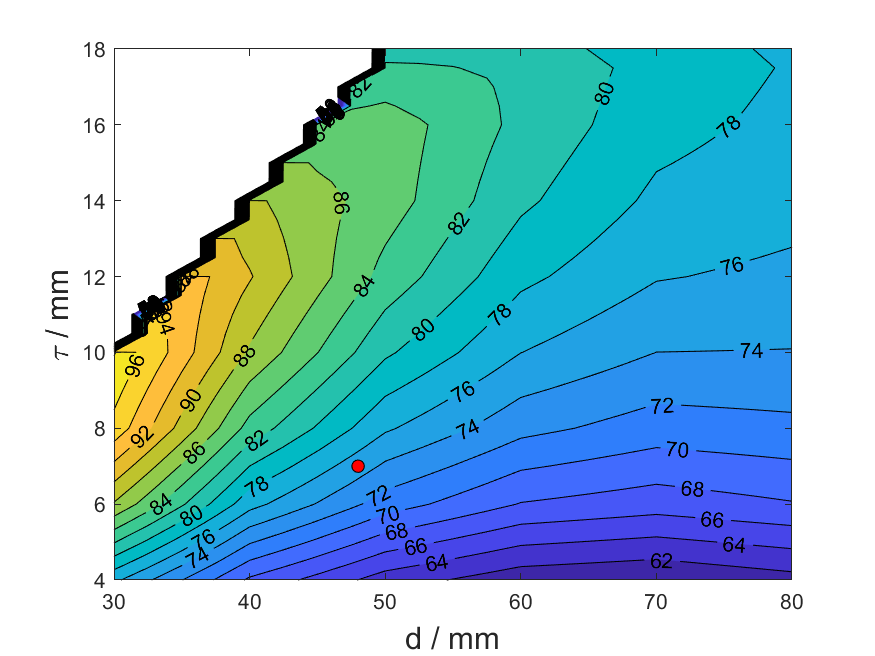
\includegraphics[width=0.48\linewidth]{helical/helical_contour_f}
    }
    \subcaptionbox[螺线管谐振腔$Q$值等高图]{螺线管谐振腔$Q$值等高图\label{fig:helical_contour_Q}}{
        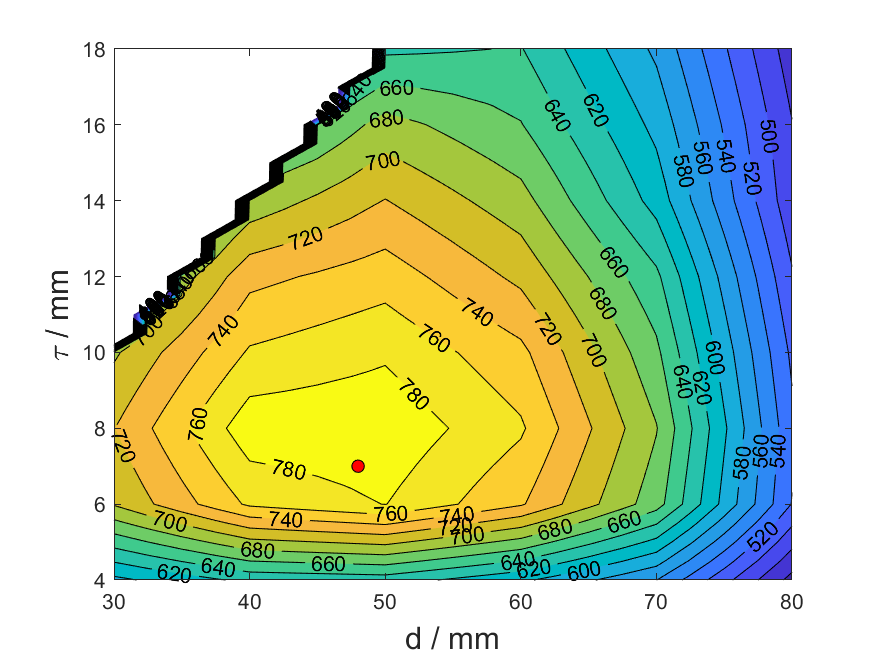
\includegraphics[width=0.48\linewidth]{helical/helical_contour_Q}
    }
\end{figure}

在图\ref{fig:helical_contour_f}中,频率$f_0$在绝大部分地方随着$\tau$的减小而减小。随着主线圈直径$d$的增加,电感$L$会先慢慢增加(当$d$较小时)然后减小(当$d$较大时)。同时,$C_c$和$C_s$单调地增加。因此在这个过程中频率会先急剧下降然后慢慢下降。参考频率计算公式\eqref{eq:helical_f_equation}和文献\cite[]{Siverns_Simkins_Weidt_Hensinger_2012,Macalpine_Schildknecht_1959}中的电感$L$和电容$C = C_c +C_s$计算公式:
\begin{align}
    L&=39.37b\frac{0.025d^2(1-(\frac{d}{D})^2)}{\tau^2} &\mu \textnormal{H/m} \label{eq:helical_L} \\
	C_c&=d(11.26\frac{b}{d}+8+\frac{27}{\sqrt{b/d}})  &\textnormal{pF/m} \label{eq:helical_C_c}\\
	C_s&=39.37b\frac{0.75}{lg(D/d)} &\textnormal{pF/m} \label{eq:helical_C_s}
\end{align}

然而,在左上和右下角,有两个非单调异常区域。一种是在大$d$和小$\tau$参数区(右下区域)。
频率等高线不是单调的,随着$d$的增大等高线向下弯曲。
这是因为当单独改变$d$时$L$有一个最大值,并且由$\tau$导致的$L$变化不足以逆转这个最大值附近的影响。另一处是在小$d$和大$\tau$参数区(左上区域)。在这里频率等高线也不是单调的,随着$\tau$的增大等高线向左弯曲(如果是将$\tau$作为横轴则是向下弯曲)。这是因为当$\tau$过大时会螺线圈会更加接近输出端会更加接近屏蔽壳引入较大的侧壁电容$C_s$而增大$\tau$带来的电感减少效应不足以抵消,从而导致频率未能随$\tau$单调增加。

对于$Q$的变化,如图\ref{fig:helical_contour_Q}所示,它具有一个明显的最大值。可见选择合适的$d$和$\tau$是十分重要的。图中$Q$的最大值位置约在$d=48$mm,$\tau=7.3$mm处,最大值$Q$约为$810$。图中红点表示了表\ref{tb:helical_simulation_parameters}中第9行的参数的$Q$值结果。

在图\ref{fig:helical_contour}的$ f_0,\ Q $结果图的帮助下,可以直接读出具有特定几何参数设置的任何$f_0$和$Q$结果。该图还可以帮助谐振腔设计和确定的$f_0$和$Q$。
此外,沿$d$或$\tau$方向任意点的偏导数将给出线圈参数对频率和$Q$的敏感性。几何参数对$f,\ Q$的敏感性决定了线圈的加工精度,以及实验误差范围。
以图\ref{fig:helical_contour}中的红点参数为例,计算线圈$d$和$\tau$灵敏度,结果如表\ref{tb:helical_d_tau_sensitivity}所示。
从结果中可以看出,灵敏度$d$的结果值小于$\tau$的结果值。因此,在加工过程中,$\tau$大小的偏差更有可能对 $f,\ Q$产生影响,值得更多地关注。

\begin{table}
    \centering
    \caption[谐振腔对主线圈直径和螺距参数的敏感性]{谐振腔对主线圈直径和螺距参数的敏感性\label{tb:helical_d_tau_sensitivity}}
    \begin{tabular}{ccccc}
        \toprule
        Operation & range (mm) & F sensitivity(MHz/mm) & Q sensitivity (/mm) \\
        \midrule
        $d$ Stretch & [-1,1] & $\approx$-0.606 & $\approx$ 0.4\\
        $\tau$ Stretch & [0, 0.5] & $\approx$ 2.988 & $\approx$ 23.491 \\
        Axial Shift & [-2, 2] & $\approx$ -0.049 & $\approx$ 0.185\\
        Radial Shift & [-2, 2] & $\approx$ 0.034 & $\approx$ -0.4904\\
        \bottomrule
    \end{tabular}
\end{table}

除了研究$f,\ Q$的独立参数变化效应外,我们还研究了主线圈平移对$f,\ Q$的影响,即沿径向或轴向。结果如图\ref{fig:helical_main_coil_compares}和表\ref{tb:helical_d_tau_sensitivity}所示。
从结果可以看出,主线圈的轴向平移和径向平移对$f,\ Q$影响不大。平移对$f,\ Q$的影响远小于几何参数 ($d,\ \tau$) 变化效应。因此,我们需要更多地关注加工过程中主线圈的俯仰精度,以获得更一致的实验结果。

\begin{figure}
    \centering
    \caption[谐振腔仿真与实验散射参数结果对比]{谐振腔仿真与实验散射参数结果对比。(a)横坐标为主线圈轴向偏移距离(单位mm),(b)主线圈平行于接地端径向偏移(单位mm),(c)主线圈垂直于接地端径向偏移(单位mm)。\label{fig:helical_main_coil_compares}}
    \subcaptionbox[主线圈轴向偏移]{主线圈轴向偏移\label{fig:helical_bias_axial}}{
        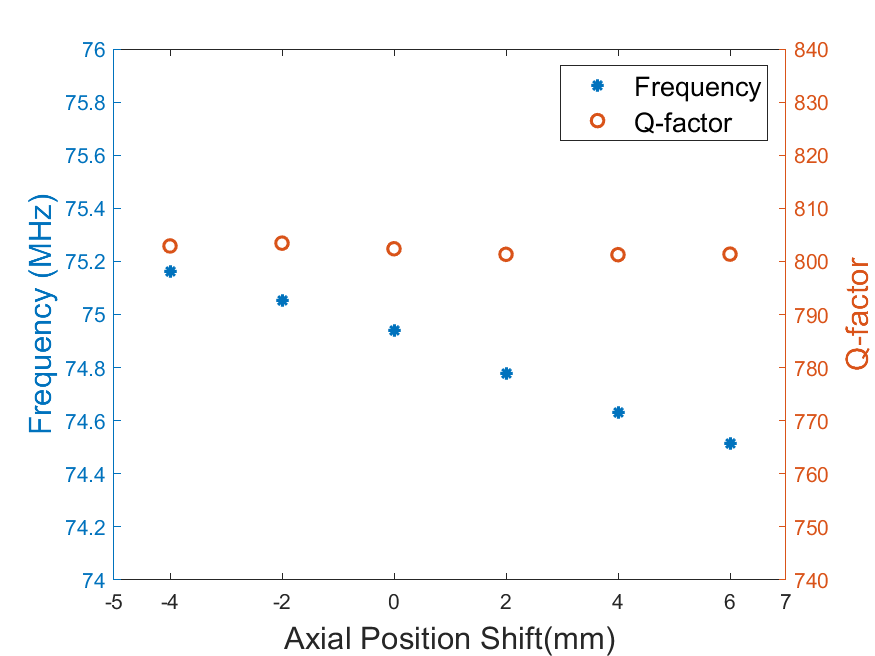
\includegraphics[width=1.0\linewidth]{helical/helical_bias_axial}
    }
    \subcaptionbox[主线圈径向偏移(平行于接地端)]{主线圈径向偏移(平行于接地端)}{
        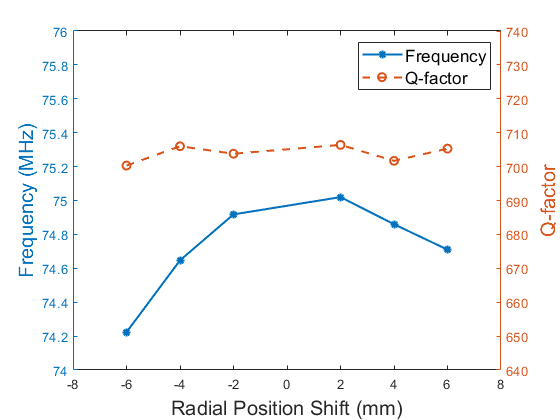
\includegraphics[width=0.46\linewidth]{helical/helical_bias_radial_gndalong}
    }
    \subcaptionbox[主线圈径向偏移(垂直于接地端)]{主线圈径向偏移(垂直于接地端)}{
        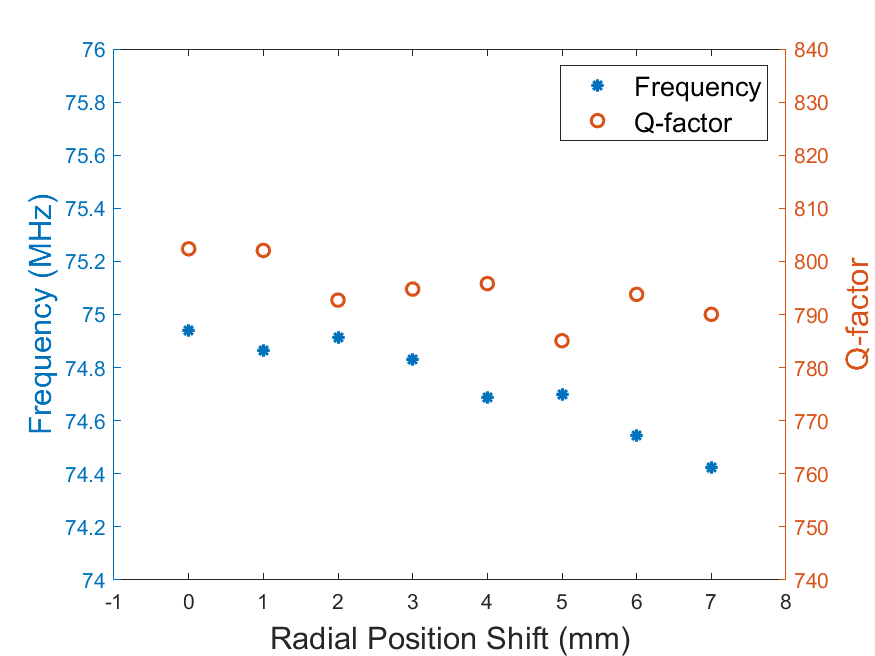
\includegraphics[width=0.46\linewidth]{helical/helical_bias_radial_gndperpendicular}
    }
\end{figure}


\subsection[输出线参数的影响]{输出线参数的影响\label{section:helical_output_wire}}
在我们的模拟中,我们发现输出导线长度对谐振$f,\ Q$有很大的影响。与之前的固定线长情况不同,这里我们不再做公式\eqref{eq:helical_fixed_constraints_1}和公式\eqref{eq:helical_fixed_constraints_2}的约束。
主线圈直径及其螺距保持在相同的长度,独立改变输出导线$l_{out}$的总长度,其中$l_{out} = l_{lout1} + l_{lout2}$。
$l_{out1}$和$l_{out2}$分别是屏蔽外壳中的输出线和连接器馈通部分的输出线,如图\ref{fig:helical_lout_2}所示。


\begin{figure}
    \centering
    \caption[输出线部分示意图]{输出线部分示意图。$l_{out1}$:输出线在屏蔽壳内部分的长度;$C_{lout1}$:输出线在屏蔽壳内部分的电容;$l_{out2}$:输出线在输出端口内部分的长度;$C_{lout2}$:输出线在输出端口内部分的电容;$D$:屏蔽壳内直径;$D_1$:输出端内直径.\label{fig:helical_lout_2}}
    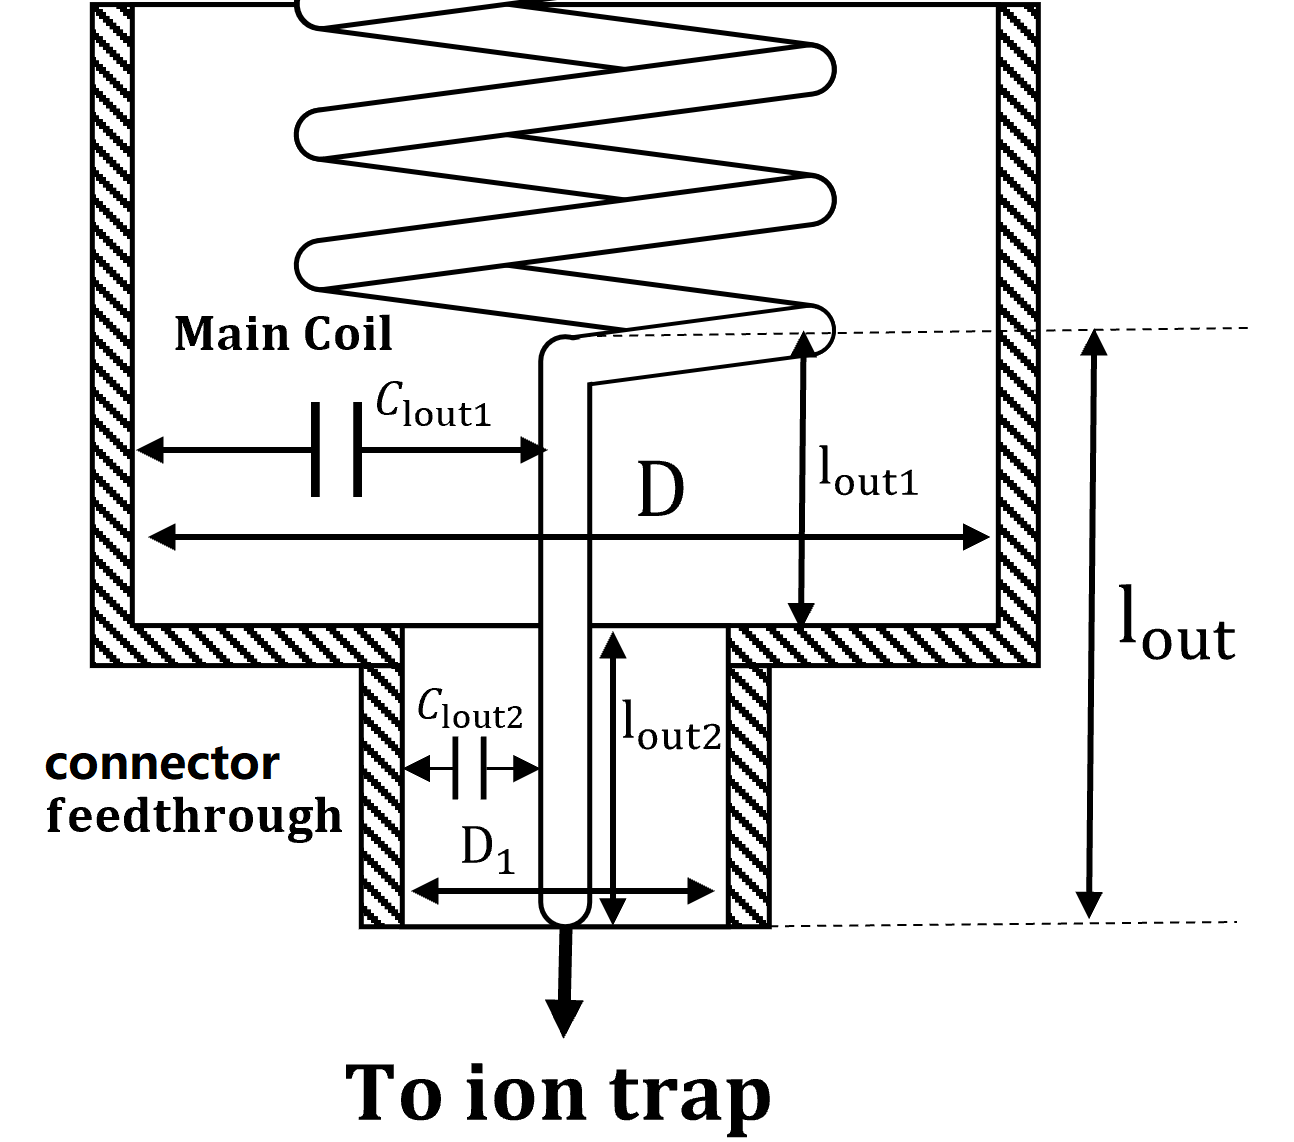
\includegraphics[width=0.6\linewidth]{helical/helical_lout_2}
\end{figure}

仿真结果如图\ref{fig:helical_lout_1}所示。随着输出导线长度的增加,谐振频率下降。$Q$随着谐振频率的减小而减小,两者成正比,与公式\eqref{eq:helical_Q_equation}具有相同的关系。这主要是输出线引入额外电容而对电阻和电感影响较小导致的。

\begin{figure}
    \centering
    \caption[输出线部分影响]{输出线部分影响。横坐标为输出线长$l_{out}$(单位mm),蓝色‘*’标和‘+’标分别为仿真和实验的频率$F$(单位MHz,对应左侧纵坐标),橙色‘o’标和‘x’标分别为仿真和实验的品质因子$Q$(单位1,对应右侧纵坐标)。\label{fig:helical_lout_1}}
    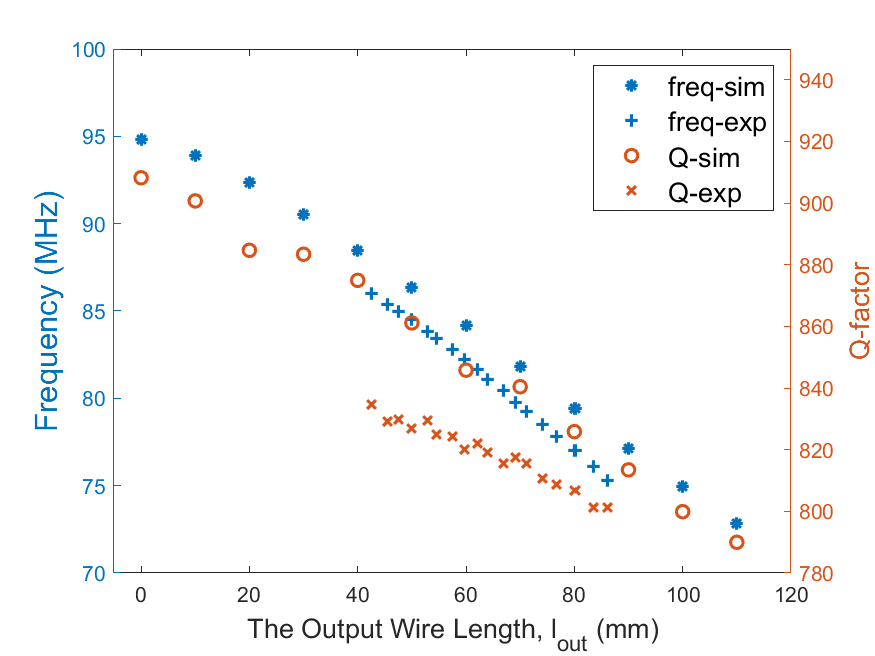
\includegraphics[width=1.0\linewidth]{helical/helical_lout_1}
\end{figure}

为了验证仿真结果,我们进行了输出导线长度切割实验,测量了输出导线长度和器件谐振频率$f_0$和$Q$。结果如图\ref{fig:helical_lout_1}所示。实验与模拟的频率差约为$2$MHz,实验测量的$Q$数据比模拟低约$150$。为了在同一图中绘制$ Q $数据,实验$ Q $数据偏移了$ 100$。除了偏移之外,频率$f_0$和$ Q $都与其对应的数据一致。该结果再次表明了仿真结果的可信度。

文献\cite[]{Gandolfi_Niedermayr_Kumph_Brownnutt_Blatt_2012,Macalpine_Schildknecht_1959, Deng_Sun_Yuan_Xu_Zhang_Lu_Luo_2014}之前研究中的理论预测和实验之间的大频率误差可能来自于忽略输出线电容\cite[]{Nandi_Sikdar_Das_Ray_2022, Batra_Panja_De_Roy_Majhi_Yadav_Sen_Gupta_2017}。我们给出了改进的LCR电路模型和一种新的电容评估公式来估计频率。与 HFSS 仿真结果相比,我们的新模型的频率预测有了很大的提高,更多细节见第\ref{section:helical_theory_model}节。

\subsection[屏蔽外壳参数的影响]{屏蔽外壳参数的影响}
\begin{figure}
    \centering
    \caption[屏蔽外壳的影响]{屏蔽外壳的影响,横坐标为屏蔽壳内直径$D$(单位mm),纵坐标为频率$F$(单位MHz)。蓝色实线和‘*’标点为频率(单位MHz,对应左侧纵坐标),橙色虚线和‘o’标点为品质因子Q(单位1,对应右侧纵坐标)。\label{fig:helical_shield_diameter}}
    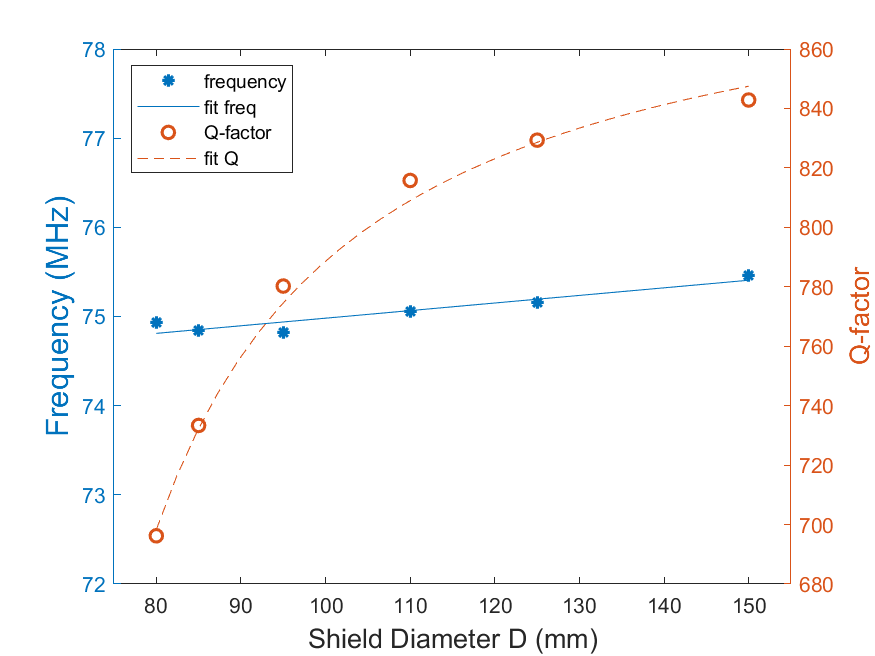
\includegraphics[width=1.0\linewidth]{helical/helical_shield_diameter}
\end{figure}

铜屏蔽外壳完成了电流回路,定义了螺旋谐振腔中的EM场边界条件。屏蔽外壳和主线圈形成电容$C_s$,因此屏蔽的直径对谐振频率有影响。屏蔽外壳可以屏蔽和减少电磁场辐射耗散,因此谐振器将具有高$Q$因子。在这里,通过数值模拟研究了屏蔽外壳直径$ D $对频率$f_0$和$ Q $因子的影响。结果如图\ref{fig:helical_shield_diameter}所示,当屏蔽直径$ D $增加时,频率$f_0$和$ Q $因子都会增加。频率变化很小,而$ Q $因子首先快速增长,然后逐渐减慢。频率的微弱增加是由于侧壁电容随着屏蔽外壳$D$的增大而减小。$Q$因子的增加是因为屏蔽直径越大,电场强度越小,屏蔽电流越小,电阻相等,耗散越小。因此为了获得更大的$Q$,在合理的设备尺寸下将首选较大的屏蔽直径。

屏蔽外壳高度的影响与相对于外壳沿轴向移动主线圈位置并相应地调整端帽位置相同。结果如图\ref{fig:helical_bias_axial}所示。屏蔽高度对频率$f_0$和$Q$因子的影响很小。

\subsection[耦合线圈参数的影响]{耦合线圈参数的影响}

耦合线圈是螺线管谐振腔的一个有趣部分。通过调节耦合线圈的形状和位置可以满足阻抗匹配工作,实现最佳耦合以最小化散射参数$S_{11}$。然而,据我们所知,以前还没有耦合线圈几何形状影响的具体相关研究。在这里,数值模拟方法提供了研究这些问题的机会。

\begin{figure}
    \centering
    \caption[耦合线圈的影响]{耦合线圈的影响。$\Delta h$:耦合线圈和主线圈之间的距离(单位mm);$d$:耦合线圈的直径(单位mm);$\tau$:耦合线圈的螺距(单位mm)。\label{fig:helical_primary_coil}}
    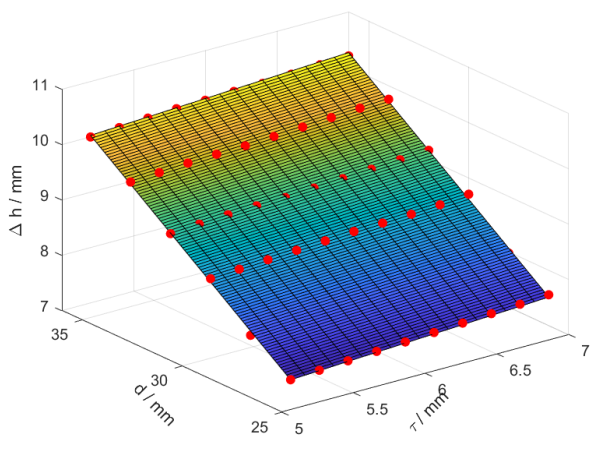
\includegraphics[width=1.0\linewidth]{helical/helical_primary_coil}
\end{figure}

为了研究主线圈形状效应,我们在其他参数满足表\ref{tb:helical_simulation_parameters}中第9行的情况下,模拟了各种耦合线圈尺寸(耦合线圈直径$d_1$和螺距$\tau_1$)及其轴向位置,并试图满足阻抗匹配。
对于每个耦合线圈(直径$d_1$和螺距$\tau_1$),扫描和优化耦合线圈在轴向的位置,以实现最小耦合反射$S_{11}$。
如果$S_{11}$系数可以达到$-45$dB或更低,认为阻抗匹配过程完成,同时记录耦合线圈轴向位置。仿真结果如图\ref{fig:helical_primary_coil}所示。
$x$轴和$y$轴分别为直径$d_1$和俯仰$\tau_1$,$z$轴为耦合线圈达到最佳耦合条件时的轴向位置。
结果表明,所有$ d_1,\ \tau_1 $参数设置都具有最佳的耦合位置$ \delta_1$,几乎所有数据点($d_1,\tau_1\delta_1$)都位于同一平面表面上。
这意味着耦合线圈的绝对形状对于实现阻抗匹配过程并不重要。总可以通过调整耦合线圈轴向位置来补偿耦合线圈的所有变形形状。

\section{谐振腔耦合过程特性}
谐振腔的实际使用离不开一个十分重要的过程,即阻抗匹配,我们一般称为耦合。经验上来看,我们知道可以通过移动耦合线圈和主线圈之间的距离或者改变耦合线圈的形状来实现耦合。一般来说实践上我们更倾向于改变耦合线圈和主线圈之间的距离的方式来实现耦合,存在一个最优距离使得匹配最佳,两者的距离太近或者太远都无法实现最佳匹配。只有在最佳匹配的时候微波功率透过谐振腔的传输率才能达到最大。在耦合的过程中谐振腔的最佳耦合频率会发生微小的偏移,而Q值则会发生较大的变化。值得注意的是,我们发现耦合过程中最佳耦合频率点和Q值的变化并不像最佳耦合点一样有最有值,如图\ref{fig:helical_coupling_delta}所示,它们是随着耦合距离单调变化的。也就是说,在最佳耦合点左右两侧,虽然透过率都会下降,但是两侧的Q值却是大不相同的。从图\ref{fig:helical_coupling_delta}中可见最佳匹配点左右两侧的Q值差能达到一倍之多,这给我们带来的启示是:我们可以通过牺牲一定的微波功率透过率来获得更高的Q值或者相反。
\begin{figure}
    \centering
    \caption[谐振腔耦合过程特性]{谐振腔耦合过程特性。横坐标为耦合线圈到主线圈的距离$\Delta h$,左侧和右侧的纵坐标分别是品质因子数值(单位1)和散射系数值(单位dB)。其中蓝色‘o’标线是谐振腔的品质因子Q,红色‘*’标线是相应的最佳耦合时的反射系数最小值$S_{11}^{min}$,绿色‘o’标线是相应的最佳耦合时的透射系数最大值$S_{21}^{max}$。\label{fig:helical_coupling_delta}}
    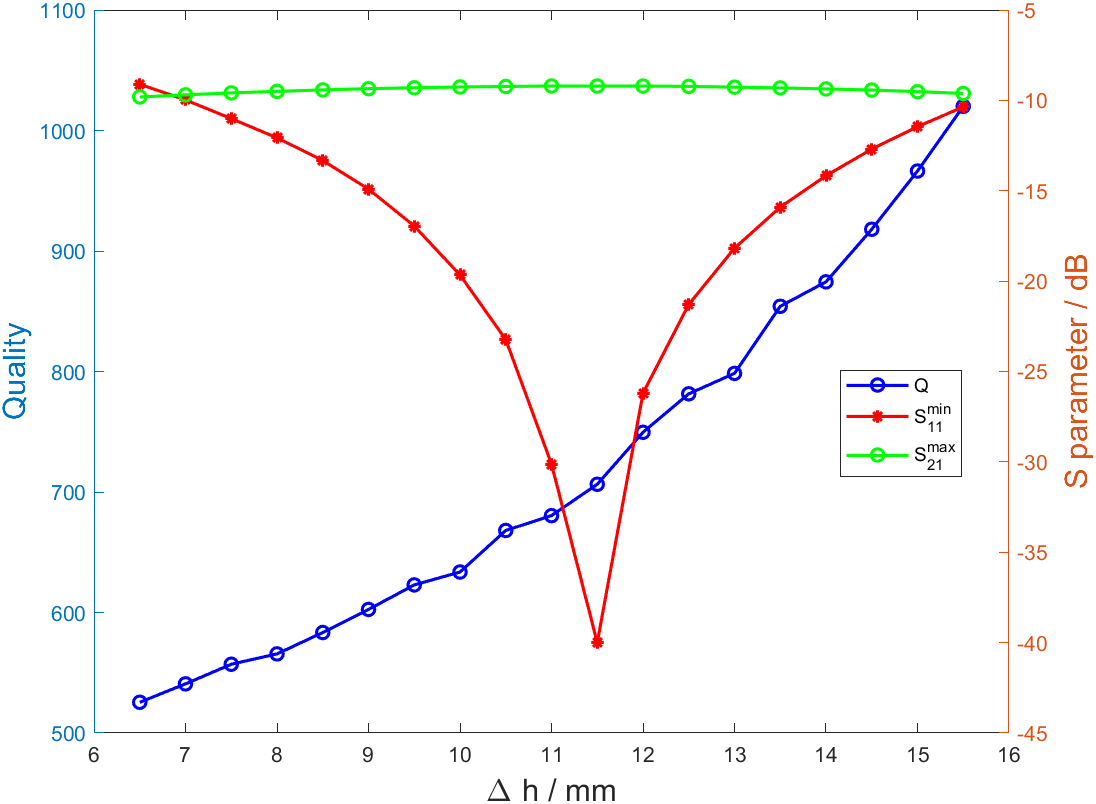
\includegraphics[width=0.8\linewidth]{helical/helical_coupling_delta}
\end{figure}

从上面的耦合过程结果来看,耦合线圈距离主线圈距离越远的情况下Q值越高。也就是说两者相互‘影响’越小的情况下Q值会越高。这个影响实际上就是等效的阻抗带来的耗散,为了验证这一点我们进行了另一组仅改变耦合线圈电阻值的实验,结果如图\ref{fig:helical_coupling_rin}所示。从图\ref{fig:helical_coupling_rin}中可以看出,随着耦合线圈电阻值的增加,Q值逐渐下降,同时也伴随着最佳耦合频率的偏移。不难发现,增加耦合线圈电阻值的过程这个结果跟图\ref{fig:helical_coupling_delta}中耦合线圈与主线圈距离的减小过程的结果是相互对应的。
\begin{figure}
    \centering
    \caption[谐振腔耦合过程特性]{谐振腔耦合过程特性。横坐标为耦合线圈的阻值$R$,左侧和右侧的纵坐标分别是品质因子数值(单位1)和散射系数值(单位dB)。其中蓝色‘o’标线是谐振腔的品质因子Q,红色‘*’标线是相应的最佳耦合时的反射系数最小值$S_{11}^{min}$,绿色‘o’标线是相应的最佳耦合时的透射系数最大值$S_{21}^{max}$。\label{fig:helical_coupling_rin}}
    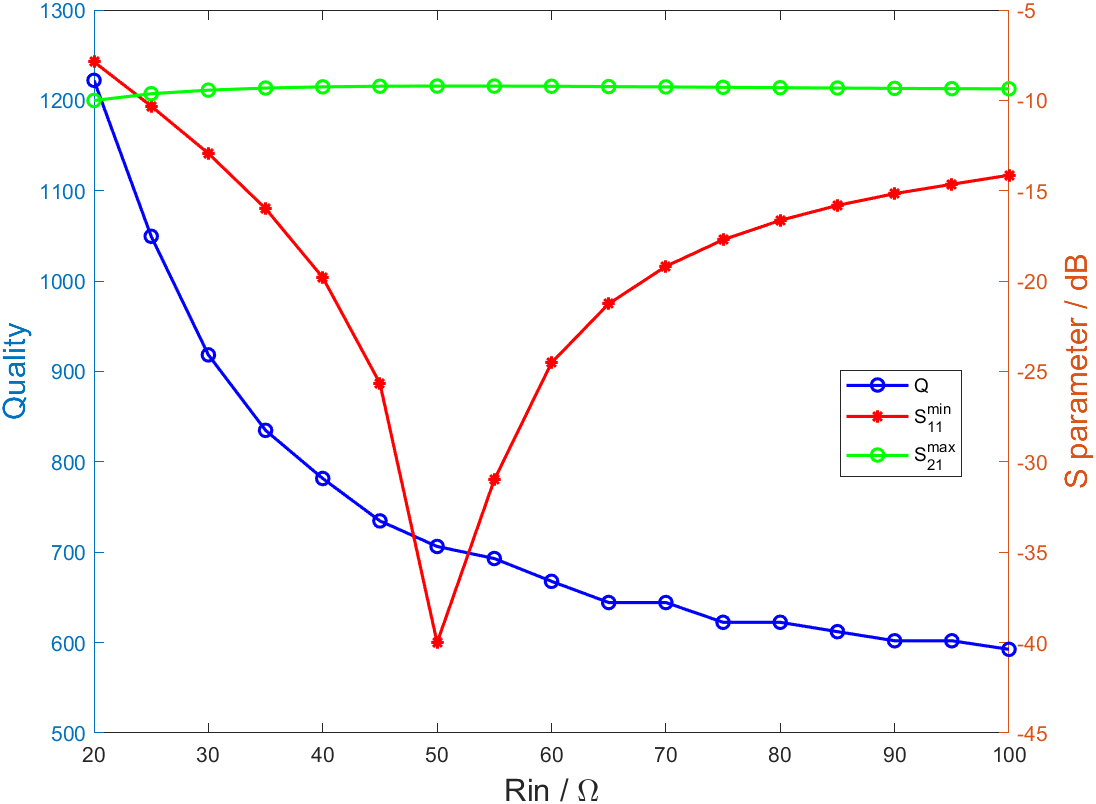
\includegraphics[width=0.8\linewidth]{helical/helical_coupling_rin}
\end{figure}


% \textcolor{red}{可以考虑将耦合过程会有不同的Q值的那个图也放上来说明一下\dots}

\newpage
\section[螺线管谐振腔的数学建模]{螺线管谐振腔的数学建模\label{section:helical_theory_model}}

螺线管谐振腔的集总电路模型可以解释和预测器件的行为。一个好的电路模型可以帮助研究人员轻松地设计具有特定属性的设备。在这里,对于螺线管谐振腔,谐振频率和较高的Q因子是最重要的两个指标。首先,对于谐振频率,我们假设额外的输出导线长度电容是频率误差发生的主要原因,如第\ref{section:helical_output_wire}节所述。

\begin{figure}
    \centering
    \caption[LCR电路模型]{LCR电路模型。$L$表示谐振腔的电感,主要包括耦合线圈和主线圈的电感;$R$表示整个谐振腔的电阻;$C$表示谐振腔的电容,$C_x$表示谐振腔内部结构的电容,$C_{lout}$表示谐振腔输出线引入的电容。\label{fig:helical_RLC_circuit1}}
    \includegraphics[width=1.0\linewidth]{helical/helical_RLC_circuit1}
\end{figure}

因此,输出线电容被添加到LCR电路模型中,如图\ref{fig:helical_RLC_circuit1}所示。总等效电容可视为传统电容CT和输出线总电容$C_{lout}$的总。传统的电容部分与以往的研究相同,而输出线和外部屏蔽将形成同轴电容:
\begin{align} 
	C_{lout}&=C_{lout1}+C_{lout2} \label{eq:helical_lout}\\ 
	C_{lout1}&=\frac{2\pi\epsilon_0 l_{out1}}{ln(D/d_0)} \label{eq:helical_lout1}\\ 
	C_{lout2}&=\frac{2\pi\epsilon_0 l_{out2}}{ln(D_1/d_0)} \label{eq:helical_lout2}
\end{align}
其中输出线电容$C_{lout1}$($C_{lout2}$)是长度为$l_{out1}$($l_{out2}$)的输出线与内径为$D$($D_1$)侧壁形成的电容。

然而,在补偿输出线长效应后,频率预测仍然低于数值模拟或实验结果。经过多次尝试,我们发现主要原因是对电容$C_c$和$C_s$的高估。最近的一项研究\cite[p52,f5.3]{article_2010}给出了一个螺线管电容$C_c$的新估计公式:
\begin{align}
    C_c=\frac{4\epsilon_0 b}{\pi}(1+k_c)/cos^2\psi 	\label{eq:helical_C_c_new}
\end{align}

其中$k_c=0.717439(d/b)+0.933048(d/b)^{3/2}+0.106(d/b)^2$,$d$是螺线管的直径,$b$是螺线管的长度,$\psi$是螺距角($\tan\psi=\tau/(\pi d)\approx 1$),$\epsilon_0$是真空介电常数。

另一方面,屏蔽壁电容$C_s$在主线圈和外部屏蔽壁之间形成,与电容$C_{lout}$相同,因此同轴电容公式可用于计算$C_s$。主线圈的等效同轴线长度为$Nd_0$,单匝等效长度为$d_0$,总主线圈有$N$匝,因此屏蔽电容计算为:

\begin{align}
    C_s=2\pi\epsilon_0 \frac{Nd_0}{ln(D/d')} \label{eq:helical_C_s_new}
\end{align}

其中$d'$是一个等效的线圈直径,$d'=d+\pi d_0/4$,其中$\pi d_0/4$是一个用于修正线圈边缘效应的因子。

此外,实际的主线圈螺旋长度有限,匝稀疏,因此需要更新或修改文献\cite[]{Siverns_Simkins_Weidt_Hensinger_2012}中的电感计算方法。短螺旋电感估计方法可计算为:

\begin{align}
    L=\frac{\mu_0 \pi (d/2)^2 }{\tau^2} (\sqrt{b^2+(d/2)^2}-d/2) \label{eq:helical_L_new}
\end{align}

最后,我们通过更新上述所有估计的方法,得到了一个新的频率预测模型。我们比较了频率预测模型、Sussex模型\cite[]{Siverns_Simkins_Weidt_Hensinger_2012}、SUST模型(本文)和 HUST模型\cite[]{Deng_Sun_Yuan_Xu_Zhang_Lu_Luo_2014}的准确性。
基于数值模拟结果,通过统计直方图对模型的有效性和准确性进行比较和评估,如图14(c)所示。频率误差的平均值和标准差越小,精度越好,误差离散越小。
所有的模型都与仿真的结果为标准做比较。
图\ref{fig:helical_freqmodelcompare}中的每一个数据结果都是一些列可行的$d,\tau$参数组合的模型预测和仿真结果的差值$\delta f=f_{model}-f_{HFSS}$,最终绘制出误差的统计分布。
针对不同的谐振频率组计算和模拟一系列离散的$d,\tau$参数(与表\ref{tb:helical_simulation_parameters}$30$MHz、$50$MHz、$75$MHz)。$d$的样本在$20-80$mm的范围内,步长为$10$mm;$\tau$的样本在$4-18$mm的范围内,步长为$2$mm。
平均偏差和标准偏差都在每个图的顶部标记。平均值是一个有符号值,表示模型的整体频率预测效果。标准差表示频率误差的离散程度。

\begin{figure}
    \centering
    \caption[三种理论模型的预测效果比较]{三种理论模型的预测效果比较。左、中、右图分别是30MHz、50MHz、75MHz附近频率设置的模型与参考表中偏差的结果的频数统计图。作为参考,每幅图上方给出了所有偏差的均值和其标准差。\label{fig:helical_freqmodelcompare}}
    \subcaptionbox[HUST模型结果]{HUST模型结果\label{fig:helical_freqmodelcompare_hust}}{
        \includegraphics[width=0.55\linewidth]{helical/helical_freqmodelcompare_hust}
    }
    \subcaptionbox[Sussex模型结果]{Sussex模型结果\label{fig:helical_freqmodelcompare_sussex}}{
        \includegraphics[width=0.55\linewidth]{helical/helical_freqmodelcompare_sussex}
    }
    \subcaptionbox[SUST模型结果]{SUST模型结果\label{fig:helical_freqmodelcompare_sust}}{
        \includegraphics[width=0.55\linewidth]{helical/helical_freqmodelcompare_sust}
    }

\end{figure}
% \begin{figure}
%     \centering
%     \caption[HUST模型结果]{HUST模型结果\label{fig:helical_freqmodelcompare_hust}}
%     \includegraphics[width=0.33\linewidth]{helical/helical_freqmodelcompare_hust}
% \end{figure}

% \begin{figure}
%     \centering
%     \caption[Sussex模型结果]{Sussex模型结果\label{fig:helical_freqmodelcompare_sussex}}
%     \includegraphics[width=0.33\linewidth]{helical/helical_freqmodelcompare_sussex}
% \end{figure}

% \begin{figure}
%     \centering
%     \caption[SUST模型结果]{SUST模型结果\label{fig:helical_freqmodelcompare_sust}}
%     \includegraphics[width=0.33\linewidth]{helical/helical_freqmodelcompare_sust}
% \end{figure}

直方图结果表明:对于$75$MHz组,本文中的模型的均值和标准差(SUST)在三个模型中都是最小的,预测的准确性是最好的。对于 $50$MHz组,SUST和HUST模型之间的平均偏差值和标准偏差值基本相似。它们都预测了比Sussex模型更准确的谐振频率。对于$30$MHz组,HUST频率预测的平均值最小,SUST模型准确率次之,但它们都优于Sussex模型。HUST和SUST模型的标准偏差相似,但它们都优于Sussex模型。需要注意的是,在30MHz组中,由于主线圈线长度约束,所有$56$种可能组合中只有$11$个可行数据,参见公式\eqref{eq:helical_fixed_constraints_1}和\eqref{eq:helical_fixed_constraints_2},因此结果可能会波动和偏差很大。

在上述结果中,对于$30-80$MHz频率范围内的情况,本文提出的LCR模型提高了预测精度。输出线效应(参见第\ref{section:helical_output_wire}节)作为对分布式电容效应的替代解释,给出了更简单直观的物理解释。

% \section[螺线管谐振腔的加工和制作]{螺线管谐振腔的加工和制作}
\newpage
\section[螺线管谐振腔的机械结构优化]{螺线管谐振腔的机械结构优化}

\subsection[旧版谐振腔]{旧版谐振腔}
旧版的谐振腔设计如图\ref{fig:helical_old_design}所示。在该设计中,主线圈的接地/直流输入端口安装在谐振腔侧壁、即主屏蔽壳上。在采用以SMA为代表的射频连接头作为端口时,会产生额外的径向长度,导致配件之间的机械冲突,安装的时候主线圈很难直接放入外筒中。装配时一般需要先将输出头向内弯折,进入筒后再进行折回,将射频接头上紧固定;或者先将射频头固定在侧壁上,装入主线圈后再进行焊接。上述两种安装方式都缺乏便利性,比如弯折过程中射频连接头焊接会脱落、或壳内焊接的复杂度较高。更重要的是,安装时往往会破坏主线圈的结构,很难完全恢复到进筒前的结构参数。还有,该设计中对主线圈的支持较弱,主线圈易形变。这在装配时会导致难以将线圈按照目标设计参数准确地进行装配,增加调试成本。即使装配好了,在工作过程中也会对外界机械抖动等较为敏感、稳定性差。该设计的耦合方式也就奥维笨拙,在实际使用中需要华为大量时间来拆卸谐振腔、调整腔内小线圈的形状来实现最佳耦合。
除此之外,该设计的主线圈输出端口的便利性、稳定性以及屏蔽性能较差。为了减小金属电容板与线圈之间的等效电容影响,通孔直径较大,使得谐振腔的信号泄露增加、屏蔽效果减弱。而谐振腔在与后级设备进行连接时,通过中空螺柱进行压接连接,稳定性较差。

为此,我们设计了一款新的谐振腔来解决以上提到的一些问题。

\begin{figure}
    \centering
    \caption[旧版的谐振腔设计]{旧版的谐振腔设计,有机械冲突、耦合方式较差。\label{fig:helical_old_design}}
    \includegraphics[width=1.0\linewidth]{helical/helical_old_design}
\end{figure}
\subsection[易装配易耦合的新版谐振腔]{易装配易耦合的新版谐振腔}
新的易装配易耦合的谐振腔设计如图\ref{fig:helical_new_design}所示。它解决了现有技术对主线圈的安装较为不便、对主线圈固定的稳定性差、对次级线圈耦合部分缺乏灵活调节的问题。新的设计主要包括以下结构:
\begin{enumerate}
    \item 主腔体屏蔽与支撑部分,包括:主屏蔽壳、底部和顶部两个固定板(记为固定板一与固定板二)、四个固定柱、一个输出屏蔽壳;
    \item 线圈及其固定与调节结构,包括:一个或两个主线圈(以下图示说明均使用两个主线圈情况、但本结构同样适用于一个主线圈的情况)、一对主线圈固定支架、一个次级线圈、一个非旋转伸缩套筒、一个射频分压电路模块;
    \item 电学相关接口与紧固零件,包括:射频输入与输出接头、直流输入接头、射频分压输出接头、及若干固定螺丝。
\end{enumerate}

新设计的实物图如图\ref{fig:helical_new_design_real}所示,将主线圈的接地/直流输入端口转移至底部固定板一。安装时可以直接固定好底座,然后将主屏蔽壳套上,再盖上顶部的固定板,最后用四个固定柱将上下两个固定板连接起来即可。安装过程不存在装配上的机械冲突。
新设计采用一对主线圈固定支架对主线圈进行支撑与固定,通过固定支架上面的凹槽设计来约束线圈为目标参数(螺线的直径、螺距、长度)。这样在装配时易按照设计目标参数进行装配,在使用过程中也能够保持稳定。
新设计巧妙地采用了非旋转伸缩套筒来实现小线圈的平动耦合。非旋转伸缩套筒可实现高精度的平动,常用于光学系统中透镜的高精度调节。套筒中心可以用来固定射频接头,并与次级线圈连接,方便次级线圈的固定和外部信号输入。非旋转伸缩套筒的表面可以镀上氧化层,形成次级线圈部分与其它部分的绝缘,很好地隔离了两者,保证了次级线圈与主线圈仅通过自由空间进行耦合,接地部分不会相互干扰。
本设计通过主线圈末端焊接射频连接头、并固定至顶部固定板,来实现谐振腔的输出。该设计中,谐振腔主腔体几乎完全封闭,增加屏蔽效果,减少腔内信号泄露、以及腔外噪声的耦入。输出为标准射频接口,与后级设备连接的便利性更高,且稳定性也有了进一步的提升。

与现有技术相比,本设计设计更为合理,元件装配更加方便,谐振耦合更加精细快捷,谐振腔长时工作的稳定性更高。
\begin{figure}
    \centering
    \caption[易装配易耦合的谐振腔设计]{易装配易耦合的谐振腔设计\label{fig:helical_new_design}}
    \includegraphics[width=1.0\linewidth]{helical/helical_new_design}
\end{figure}

\begin{figure}
    \centering
    \caption[易装配易耦合的谐振腔设计实物图]{易装配易耦合的谐振腔设计实物图\label{fig:helical_new_design_real}}
    \includegraphics[width=1.0\linewidth]{helical/helical_new_design_real}
\end{figure}
% !TeX root = ../sustechthesis-example.tex

\chapter[离子阱频率稳定]{离子阱频率稳定\label{section:trap_frequency_stablization}}

% \textcolor{red}{这部分主要介绍参考文献\cite[]{Johnson_Wong_Campos_Restelli_Landsman_Neyenhuis_Mizrahi_Monroe_2016}}

带电粒子通常由射频(RF)电势控制,其场梯度提供时间平均力,这些力构成了四极质量滤波器、离子质谱仪和射频(Paul)离子阱等应用的基础\cite[]{Dehmelt_1990, Paul_1990}。这些射频电势,通常在 1 kHz 到 100 MHz 的频率处数百或数千个伏特,在真空中驱动高阻抗负载,通常由射频放大器和谐振升压变换器(例如四分之一波或螺旋谐振器)产生\cite[]{Siverns_Simkins_Weidt_Hensinger_2012}。这种电路容易受到放大器增益、变压器的机械振动和系统中的温度漂移的波动的影响。离子阱对这些波动特别敏感,因为射频电势决定了被捕获离子的谐波振荡频率。稳定的阱频率在从量子信息处理\cite[]{Blatt_Wineland_2008, Monroe_Kim_2013}和量子模拟\cite[]{Richerme_Gong_Lee_Senko_Smith_Foss_Feig_Michalakis_Gorshkov_Monroe_2014, Jurcevic_Lanyon_Hauke_Hempel_Zoller_Blatt_Roos_2014}到原子运动的量子态的制备\cite[]{Leibfried_Blatt_Monroe_Wineland_2003}、原子干涉测量\cite[]{Johnson_Neyenhuis_Mizrahi_Wong_Campos_Monroe_2015}、和量子有限计量\cite[]{Chou_Hume_Koelemeij_Wineland_Rosenband_2010}等方面至关重要。


理论上离子阱中影响阱频率的各种因素
在离子阱系统中,阱频率的表达式为:
\begin{align}
    \omega=e\mu V_0/\sqrt{2}m\Omega R^2
\end{align}

这些参数分别是:
\begin{itemize}
    \item $e$: 离子电荷量;
    \item $\mu$: 几何效率因子;
    \item $m$: 粒子质量;
    \item $R$: 电极间距;
    \item $\Omega$: 输入微波信号的频率;
    \item $V_0$: 输入信号的电压;
\end{itemize}


上面的各个参数中$e$,$\mu$,$m$是常数,R在阱几何形状确定的情况下也是常数。因此,关键的参数在于与射频相关的 $\Omega$ 和 $V_0$ 。这其中,当今射频生成器件自身的频率和幅度稳定性是相当高的,可能产生抖动因素的实际上主要是经过谐振腔后的输出幅度。我们使用的螺线管谐振腔$Q$值较高,只要谐振腔的中心透过频率稍微发生偏移,输出幅度就可能发生较大的抖动。因此阱频稳定主要是通过稳定谐振腔输出的射频幅度实现的。

% 物理上离子阱中影响阱频率的各种因素



\section[离子阱频率稳定原理]{离子阱频率稳定原理}
受环境振动和温度变化影响,谐振腔的几何形状,主要是螺旋线的长度和腔体长度会发生变化,进而导致谐振腔的中心频率发生偏移。从谐振腔的S参数图\ref{fig:helical_compares}中可以看出螺线管谐振腔的Q值很大,透过峰较尖锐,即中心频率附近信号透过衰减较大。因此在输入信号频率抖动极小的情况下,受谐振腔中心频率偏移影响,信号的透过幅度将会发生较大的变化。
文献\cite[]{Johnson_Wong_Campos_Restelli_Landsman_Neyenhuis_Mizrahi_Monroe_2016}中介绍了采用模拟系统实现的离子阱频率稳定方案。该方案的简化版采用了鉴频器、射频功率放大器、模拟PID控制器、电容分压器、混频器、本地振荡源等器件。采用模拟方案涉及到的器件较多、灵活性差,因此我们采用基于数字系统的稳定方式。

基于RTMQ系统的数字PID离子阱频率稳定原理图如图\ref{fig:trap_frequency_lock}所示。信号通过PID对DDS进行幅度调制产生,随后经过射频功率放大器进入谐振腔耦合输入端。通过调节谐振腔耦合输入端对谐振腔进行阻抗匹配耦合,使得输出功率最大化。随后,在输出端焊接一个射频分压电路,按照100:1的分压比采集射频电压作为检测信号送入鉴频器。接着鉴频器的输出接入RTMQ板卡的16位AD转换芯片,进而转换成数字信号作为PID输入,完成整个控制回路闭环。其中,分压电路图如图\ref{fig:trap_frequency_lock}中小图所示,$C_1=C_2\approx10$uF用于同步两个输出端的射频相位;$C_3\approx0.5$pF,$C_4\approx50$pF构成理论上为$100:1$射频分压电路(实际上受到焊接电容影响测得的分压比约为$53:1$)。

\begin{figure}
    \centering
    \caption[数字PID离子阱频率稳定原理图]{基于RTMQ系统的数字PID离子阱频率稳定原理图。DDS:数字频率发生器;PID:比例微分积分控制器;ADC:模拟数字转换器;$C_1,C_2$:相位同步电容;$C_3,C_4$:射频分压电容。\label{fig:trap_frequency_lock}}
    \includegraphics[width=1.0\linewidth]{trap_frequency_lock}
\end{figure}


\section[离子阱频率稳定系统搭建]{离子阱频率稳定系统搭建}

由于系统中需要使用放大器,而放大器对不同频率的信号放大效果有所区别。过大的放大信号可能会损坏谐振腔的分压板,因此这里先用DDS的输出和放大器预先对放大器进行标定,结果如图\ref{fig:helical_lock_amplifier}所示。从结果图中的拟合直线截距上可以看出,信号功率放大器可以对信号放大约32.83dBm。

\begin{figure}
    \centering
    \caption[DDS输出功率和放大器输出功率]{DDS输出功率和放大器输出功率。横坐标为DDS输出功率(单位dBm),纵坐标为测量得到的放大后的射频功率(单位dBm)。蓝色实心点是测得的数据点,蓝色虚线是从数据点中拟合出的直线,系数$a=0.9644$,截距$b=32.83$表示功率放大器的放大dBm数。\label{fig:helical_lock_amplifier}}
    \includegraphics[width=1.0\linewidth]{helical_lock_amplifier}
\end{figure}

阱频稳定模块实验测试图如附录图\ref{fig:trap_frequency_lock_real}所示。

\section[离子阱频率稳定系统结果]{离子阱频率稳定系统结果}

谐振腔输出稳定效果测量结果如图\ref{fig:helical_lock_measure}所示,蓝色测量数据是在未进行稳定时测的的谐振腔输出幅度与输入功率设定值的关系,橙色和灰色测量数据分别为将数字PID控制器目标值设定为-638和-909时的测量结果。在未稳定的情况下,谐振腔的输出幅度会跟随外部输入信号的幅度变化而变化,呈现出一定的比率关系。如图中蓝色测量数据,其斜率约为244.55;经过稳定后,在大范围内谐振腔的输出幅度仍然会跟随外部输入信号的幅度变化而变化,不过其呈现的比例关系会受到稳定抑制作用而减小,如图中橙色和灰色测量数据,其斜率在155附近。从中可见,添加数字PID控制器对谐振腔的输出幅度会有明显的稳定抑制作用。

\begin{figure}
    \centering
    \caption[谐振腔输出稳定效果测量结果]{谐振腔输出稳定效果测量结果。横坐标为DDS的设定输出功率数字值(非实际功率值),纵坐标我板卡上ADC测得的输出电压数字值(非实际功率值)。该图个数据点测量的是PID参考功率数值一定的情况下,改变输入的射频功率大小,看实际输出功率大小的变化。整体上斜率越小表明控制器对功率大小的变化有抑制作用。\label{fig:helical_lock_measure}}
    \includegraphics[width=1.0\linewidth]{helical_lock_measure}
\end{figure}



% !TeX root = ../sustechthesis-example.tex

\chapter[脉冲激光拍频锁定]{脉冲激光拍频锁定}

\textcolor{red}{这部分叙述主要参考文献\cite[]{Islam_Campbell_Choi_Clark_Conover_Debnath_Edwards_Fields_Hayes_Hucul_et_al_2014}}

\section[脉冲激光拍频锁定原理]{脉冲激光拍频锁定原理}

\section[脉冲激光拍频锁定系统搭建]{脉冲激光拍频锁定系统搭建}

\section[脉冲激光拍频系统锁定结果]{脉冲激光拍频系统锁定结果}


% !TeX root = ../sustechthesis-example.tex

\chapter[激光功率稳定]{激光功率稳定}
\section[激光功率稳定]{激光功率稳定}
在离子阱量子计算中,激光功率稳定非常重要,因为激光功率的波动会影响离子阱中囚禁离子的运动和量子态\cite[]{Blums_Scarabel_Shimizu_Ghadimi_Connell_Händel_Norton_Bridge_Kielpinski_Lobino_et_al_2020}。具体来说,激光功率稳定有以下几个作用:
\begin{enumerate}
    \item 提高量子比特的质量:激光功率稳定可以减少离子阱中囚禁离子的运动和量子态的噪声,从而提高量子比特的质量和精度;
    \item 延长量子比特的寿命:激光功率稳定可以减少离子阱中囚禁离子的能量损失,从而延长量子比特的寿命;
    \item 提高量子计算的成功率:激光功率稳定可以减少离子阱中囚禁离子的运动和量子态的噪声,从而提高量子计算的成功率;
    \item 实现精确的量子操作:激光功率稳定可以实现精确的量子操作,例如囚禁离子的冷却、囚禁离子的量子门操作等;
    \item 
\end{enumerate}

因此,在离子阱量子计算中,保持激光功率稳定是非常重要的,可以提高量子比特的质量、延长量子比特的寿命、提高量子计算的成功率和实现精确的量子操作。



\section[激光功率外部稳定原理]{激光功率外部稳定原理}
激光功率稳定与多种因素有关,通常来说有温度控制、电流控制、光学反馈控制、机械稳定性等,这些因素基本都针对激光器本身进行稳定。除了对激光器本身进行稳定外,还可以激光输出的后续光路中设计相关的控制系统对激光进行稳定。这种方式独立于激光器吱声的出光稳定,可以在激光出光稳定的基础上进一步提高激光功率的稳定性。下面介绍这种激光功率外部稳定原理和实现。

\begin{figure}
    \centering
    \caption[激光功率外部稳定]{激光功率外部稳定\label{fig:laser_stabilization0}}
    \includegraphics[width=1.0\linewidth]{laser_stabilization0}
\end{figure}

整个激光功率外部稳定系统主要包括如图\ref{fig:laser_stabilization0}几部分:激光器、透镜组、半波片HWP、光偏振分束镜PBS、光功率分配镜PS(B)、声光调制器AOM、光分束镜PS(B)、光子探测器PD、ADC芯片、数字PID、直接数字信号合成器DDS、射频功放PA、射频功率分配器PS(RF)。

整个过程如下,首先激光器产生激光经过透镜和反光镜组将激光变换到要求的光斑大小和入射位置;接着使用半波片(HWP)将光转化为垂直和水平偏振成分;接着使用偏振分数器将偏振光提纯为匹配AOM偏振需求的光;随后使用光功率分配器分出一部分激光用于构成反馈回路,另一部分光经过控制回路控制的AOM调制后成为可用的功率稳定激光;激光经过AOM后会产生若干级衍射光,起哄主要能量集中在0级和1级衍射光上,我们可以选择其中一路来进行探测和稳定(这里选择1级光);将一级光经过光功率分束镜一部分作为测试监测,另一部分用于反馈控制回路中。控制器采用基于RTMQ板卡数字系统实现,主要器件为ADC、数字PID、DDS,除此之外还需要功率放大器(PA)和射频功率分配器(可选,如果只有一路则不用,实际使用中可以分出多路来调控多了AOM)。通过调节射频功率的大小可以控制AOM1级光和0级光的功率分布,在合理范围内,功率越大1激光分得的功率越高。数字PID根据1级衍射光的功率变化控制DDS输出不同功率的射频信号,从而实现对1级衍射激光的稳定。

对于整个控制回路,一般来说只需要分出两路如AOM0和AOM1,一路AOM0用来做功率稳定的反馈回路,另一路AOM1用来做工作光,然后可以拓展地在另一路后面添加光功率分配镜来获得更多路的稳定光,如附录图\ref{fig:laser_stabilization}所示。


\section[激光功率锁定系统搭建]{激光功率锁定系统搭建}
激光功率锁定系统测试如附录图\ref{fig:laser_stabilization_real}所示。


\section[激光功率锁定系统结果]{激光功率锁定系统结果}
% D:\Database\Files\2021-2024-研究生事件文件\2022-2023\研究\2023年4月13日-光功率稳定\2023年4月27日_光功率计测试数据

数据的测量采用如图所示的RIGOL示波器进行,在50kHz的采样率下采集约3.5s的数据。激光功率外部稳定本底、稳定前、稳定后原始数据如图\ref{fig:laser_stabilization_data}所示,从图中看可以看出PD在无激光输入的暗态下本底噪声较小。除此之外,可以看到经过稳定后的激光功率小于稳定前的激光功率,这其中的主要原因是稳定过程中AOM动态分离了部分激光功率。为了能够有效地对比稳定前后的效果,我们用各组数据的均值对功率测试的结果进行归一化处理$P_{norm}=P_{orignal}/mean(P_{orignal})$,结果如图\ref{fig:laser_stabilization_data0}所示。由于本底噪声过于接近0,因此本底噪声的归一化结果呈现发散状态,在这里不具有参考价值。从图\ref{fig:laser_stabilization_data0}中可以明显看出经过数字PID稳定系统后的功率更加稳定了。

\begin{figure}
    \centering
    \caption[激光功率外部稳定原始数据]{激光功率外部稳定本底、稳定前、稳定后原始数据\label{fig:laser_stabilization_data}}
    \includegraphics[width=1.0\linewidth]{laser_stabilization_data}
\end{figure}

\begin{figure}
    \centering
    \caption[激光功率外部稳定归一化后数据]{激光功率外部稳定归一化后本底、稳定前、稳定后数据\label{fig:laser_stabilization_data0}}
    \includegraphics[width=1.0\linewidth]{laser_stabilization_data0}
\end{figure}

一般来说可以通过计算两组数据归一化后的方差之比可以粗略地获得稳定效果,方差越小稳定性越高。经计算稳定前后激光功率数据的方差比为$\frac{\sigma_{unstable}}{\sigma_{stabled}}\approx 9.17$。整体上经过激光功率稳定系统后,稳定前好了约9倍。为了能够更加直观地评估稳定的效果,我们将归一化后的所有数据点绘制出统计柱状图(由于本底的归一化不具有参考价值因此这里省略),结果如图\ref{fig:laser_stabilization_data1}所示。
\begin{figure}
    \centering
    \caption[激光功率外部稳定柱状图对比数据]{激光功率外部稳定归一化后本底、稳定前、稳定后数据柱状图。\label{fig:laser_stabilization_data1}}
    \includegraphics[width=0.8\linewidth]{laser_stabilization_data1}
\end{figure}

为了能更好了解稳定效果的长时间表现情况,我们重新以3Hz的采样率采集了一组长期数据,并绘制出了归一化后稳定前后数据的阿兰方差,如图\ref{fig:laser_stabilization_data2}所示。从结果对比来看,稳定后的激光功率数据的阿兰方差在各个滑动窗口都低于未稳定时的。表明这里的数字稳定系统在较长时间的各个滑动窗口稳定性都好于未稳定时的。
\begin{figure}
    \centering
    \caption[激光功率外部稳定阿兰方差对比数据]{激光功率外部稳定归一化后本底、稳定前、稳定后数据阿兰方差。\label{fig:laser_stabilization_data2}}
    \includegraphics[width=0.8\linewidth]{laser_stabilization_data2}
\end{figure}



% !TeX root = ../sustechthesis-example.tex

\chapter[离子阱频率锁定]{离子阱频率锁定}

% \textcolor{red}{这部分主要介绍参考文献\cite[]{Johnson_Wong_Campos_Restelli_Landsman_Neyenhuis_Mizrahi_Monroe_2016}}

带电粒子通常由射频(RF)电势控制,其场梯度提供时间平均力,这些力构成了四极质量滤波器、离子质谱仪和射频(Paul)离子阱等应用的基础\cite[]{Dehmelt_1990, Paul_1990}。这些射频电势,通常在 1 kHz 到 100 MHz 的频率处数百或数千个伏特,在真空中驱动高阻抗负载,通常由射频放大器和谐振升压变换器(例如四分之一波或螺旋谐振器)产生\cite[]{Siverns_Simkins_Weidt_Hensinger_2012}。这种电路容易受到放大器增益、变压器的机械振动和系统中的温度漂移的波动的影响。离子阱对这些波动特别敏感,因为射频电势决定了被捕获离子的谐波振荡频率。稳定的阱频率在从量子信息处理\cite[]{Blatt_Wineland_2008, Monroe_Kim_2013}和量子模拟\cite[]{Richerme_Gong_Lee_Senko_Smith_Foss_Feig_Michalakis_Gorshkov_Monroe_2014, Jurcevic_Lanyon_Hauke_Hempel_Zoller_Blatt_Roos_2014}到原子运动的量子态的制备\cite[]{Leibfried_Blatt_Monroe_Wineland_2003}、原子干涉测量\cite[]{Johnson_Neyenhuis_Mizrahi_Wong_Campos_Monroe_2015}、和量子有限计量\cite[]{Chou_Hume_Koelemeij_Wineland_Rosenband_2010}等方面至关重要。


理论上离子阱中影响阱频率的各种因素
在离子阱系统中,阱频率的表达式为:
\begin{align}
    \omega=e\mu V_0/\sqrt{2}m\Omega R^2
\end{align}

这些参数分别是:
\begin{itemize}
    \item $e$: 离子电荷量;
    \item $\mu$: 几何效率因子;
    \item $m$: 粒子质量;
    \item $R$: 电极间距;
    \item $\Omega$: 输入微波信号的频率;
    \item $V_0$: 输入信号的电压;
\end{itemize}


上面的各个参数中$e$,$\mu$,$m$是常数,R在阱几何形状确定的情况下也是常数。因此,关键的参数在于与射频相关的 $\Omega$ 和 $V_0$ 。这其中,当今射频生成器件自身的频率和幅度稳定性是相当高的,可能产生抖动因素的实际上主要是经过谐振腔后的输出幅度。我们使用的螺线管谐振腔$Q$值较高,只要谐振腔的中心透过频率稍微发生偏移,输出幅度就可能发生较大的抖动。因此阱频稳定或者说阱频锁定主要是通过稳定谐振腔输出的射频幅度实现的。

% 物理上离子阱中影响阱频率的各种因素

受环境振动和温度变化影响,谐振腔的几何形状,主要是螺旋线的长度和腔体长度会发生变化,进而导致谐振腔的中心频率发生偏移。从谐振腔的S参数图中可以看出螺线管谐振腔的Q值很大,透过峰较尖锐,即中心频率附近信号透过衰减较大。因此在输入信号频率抖动极小的情况下,受谐振腔中心频率偏移影响,信号的透过幅度将会发生较大的变化。

\section[离子阱频率锁定原理]{离子阱频率锁定原理}

\section[离子阱频率锁定系统搭建]{离子阱频率锁定系统搭建}

由于系统中需要使用放大器,而放大器对不同频率的信号放大效果有所区别。过大的放大信号可能会损坏谐振腔的分压板,因此这里先用DDS的输出和放大器预先对放大器进行标定,结果如图\ref{fig:helical_lock_amplifier}所示。从接种的拟合直线截距上可以看出,信号功率放大器可以对信号放大月32.83dBm。

\begin{figure}
    \centering
    \caption[DDS输出功率和放大器输出功率]{DDS输出功率和放大器输出功率\label{fig:helical_lock_amplifier}}
    \includegraphics[width=1.0\linewidth]{helical_lock_amplifier}
\end{figure}

阱频锁定模块实验测试图如附录图\ref{fig:trap_frequency_lock_real}所示。

\section[离子阱频率锁定系统结果]{离子阱频率锁定系统结果}


谐振腔输出锁定效果测量结果如图\ref{fig:helical_lock_measure}所示。

\begin{figure}
    \centering
    \caption[谐振腔输出锁定效果测量结果]{谐振腔输出锁定效果测量结果\label{fig:helical_lock_measure}}
    \includegraphics[width=1.0\linewidth]{helical_lock_measure}
\end{figure}



% !TeX root = ../sustechthesis-example.tex

\chapter[脉冲激光操控离子(量子门)实验]{脉冲激光操控离子(量子门)实验}

\textcolor{red}{
这章看情况,如果实验系统跟得上的话加上,具体实验设计留再讨论...
}

\section[态初始化保真度]{态初始化保真度}

\section[XXXX]{XXXX}

\section[XXXX]{XXXX}

\section[XXXX]{XXXX}

\section[XXXX]{XXXX}



% 结论
\backmatter
% !TeX root = ../sustechthesis-example.tex

\begin{conclusion}

量子计算拥有着广阔的发展和应用前景。离子阱量子计算因其较高的相干时间和保真度是量子计算未来重要的发展方向之一。

\end{conclusion}





% 参考文献
\bibliography{ref/refs}  % 参考文献使用 BibTeX 编译
% \printbibliography       % 参考文献使用 BibLaTeX 编译(兼容性不佳,不太推荐)

% 附录
\appendix
% !TeX root = ../sustechthesis-example.tex

\chapter{补充内容}

% 一些数学、图片、表格、代码等的补充... 

\begin{figure}
    \centering
    \caption[8位超前进位加法器的FPGA实现结构图]{8位超前进位加法器的FPGA实现结构图(Vivado)\label{fig:ahead_adder_8bits}}
    \includegraphics[width=1.0\linewidth]{rtmq/ahead_adder_8bits}
\end{figure}

\begin{figure}
    \centering
    \caption[16位超前进位加法器的FPGA实现结构图]{16位超前进位加法器的FPGA实现结构图(Vivado)\label{fig:ahead_adder_16bits}}
    \includegraphics[width=1.0\linewidth]{rtmq/ahead_adder_16bits}
\end{figure}


\begin{figure}
    \centering
    \caption[32位Booth乘法器编码和加法树表]{32位Booth乘法器编码和加法树表\label{fig:booth_multiplier_32bits_basic}}
    \includegraphics[width=1.0\linewidth]{rtmq/booth_multiplier_32bits_basic}
\end{figure}

\begin{figure}
    \centering
    \caption[脉冲激光拍频锁定系统图]{脉冲激光拍频锁定系统图\label{fig:beat_note_stabilization_real}}
    \includegraphics[width=1.0\linewidth]{beat_note_stabilization_real}
\end{figure}

\begin{figure}
    \centering
    \caption[阱频锁定模块实验测试图]{阱频锁定模块实验测试图\label{fig:trap_frequency_lock_real}}
    \includegraphics[width=1.0\linewidth]{trap_frequency_lock_real}
\end{figure}

\begin{figure}
    \centering
    \caption[激光功率锁定系统测试图]{激光功率锁定系统测试图\label{fig:laser_stabilization_real}}
    \includegraphics[width=1.0\linewidth]{laser_stabilization_real}
\end{figure}

\begin{figure}
    \centering
    \caption[激光功率外部稳定的拓展方案架构图]{激光功率外部稳定的拓展方案架构图\label{fig:laser_stabilization}}
    \includegraphics[width=1.0\linewidth]{laser_stabilization1}
\end{figure}

% 致谢
% !TeX root = ../sustechthesis-example.tex

\begin{acknowledgements}
  衷心感谢导师张君华副研究员和量子院路尧、王钊副研究员、张丽昀助理教授等对本人的精心指导,老师们的言传身教将使我终生受益。

  依稀记得刚来实验室时君华老师对我的真切关怀,那时候对深圳这座城市完全是陌生的,对将要从事的离子阱量子计算领域的研究也是半知半解的。十分感谢君华老师带我熟悉深圳和实验室的环境,并且给我推荐了如《量子力学概论》、《量子信息》、《Atom》等领域相关的书籍作为入门学习。这些书籍为我随后在离子阱量子计算方向的研究打下了很好的基础。与此同时,路尧老师在经常会在实验室白板上分享有关光与离子相互作用的知识。这些知识十分具体,将从前在书本上学习到的许多量子的概念结合离子阱这个系统进行了具象化。路老师的这些分享帮助了我快速熟悉和了解离子阱量子计算整个系统的原理和实验,使我受益匪浅。在研一下学期到研二期间,十分荣幸能够与王钊老师一起合作关于用于离子阱系统的螺线圈谐振腔的研究。这是我着手的第一个真正意上的研究工作。我们从文献阅读到仿真模拟,再到实验制作与验证以及随后的理论模型的建立等等。在此期间王老师给了我许多有益的建议和帮助,比如在实验前要做好充分的准备、每次实验要有良好的计划和预期、如何合理规划实验与数据处理的时间等等。与王老师的合作初步建立起了我对科研项目的整体认识。在研二和三期间与君华老师、路尧老师、王钊老师一起进行脉冲激光实现离子量子门方案的实验平台的过程中,君华老师在RTMQ系统的开发和使用上给了我很大的支持,包括检查代码问题、测控板问题等等;路尧老师和王钊老师分别在整体系统架构和原理方面,以及离子的囚禁和真空系统方面给了我很大的帮助。尽管受到各种限制没能最终完全实现基于脉冲激光的离子量子门的整个系统的搭建和测试而有些遗憾,在搭建诸如激光功率稳定、脉冲激光拍频锁定、捕捉离子、测控系统开发、谐振腔等等重要的子系统的过程中也学到了许多宝贵的知识,积累了丰富的经验,为以后的研究打下了坚实的基础。在整个研究期间,张丽昀老师在实验室布局、器件采购和实验设备的使用上一直细心耐心地安排,给了我许多指导。
  
  作为一个新的实验组,组里的各位老师都朝气磅礴,作为组里的第一名学生,我深受各位老师们的感染。老师们在离子阱量子计算领域专业的素养、乐于分享的精神、乐观开朗的态度、精益求精的品质等等,在科研过程中一直都潜移默化地影响着我,使我取得了巨大的成长和进步。再次感谢各位老师的引导和陪伴!

  % 在美国麻省理工学院化学系进行九个月的合作研究期间,承蒙 Robert Field 教授热心指导与帮助,不胜感激。

  % 感谢×××××实验室主任×××教授,以及实验室全体老师和同窗们学的热情帮助和支持!

  最后,感谢父母、家人还有各位同学朋友的关爱和支持,亲人的期望和祝福是我前进的不竭动力,同学朋友们的陪伴和交流使我的研究生生活更加丰富多彩。感谢一路有你们,你们永远在我心中!

  % 本课题承蒙国家自然科学基金资助,特此致谢。
\end{acknowledgements}


% 个人简历、在学期间完成的相关学术成果
% !TeX root = ../sustechthesis-example.tex

\begin{resume}

  \section*{个人简历} % 根据正文撰写语言选择

  1998年04月,出生于河南省南阳市邓州市;

  2017年09月,考入山东大学机电与信息工程学院学习;
  
  2021年06月,本科毕业并获得通信工程学士学位;

  2021年09月,进入南方科技大学量子科学与工程研究院学习;
  
  2024年06月,研究生毕业并电子科学与技术硕士学位;

  \textbf{获奖情况:}

  2021年12月,获“华为杯”第十八届中国研究生数学建模竞赛国家级三等奖;

  2022年02月,获第十三届“挑战杯”广东大学生创业计划竞赛优秀奖;

  2023年11月,获南方科技大学研究生国家奖学金;
  
  % 如获三好学生、优秀团干部、×奖学金等(不含科研学术获奖)。

  % 工作经历:……

  % \section*{Resume} % 根据正文撰写语言选择
  % FamilyName GivenName was born in 1997, in Shenzhen, Guangdong, China.

  % In September 2015, he/she was admitted to Southern University of Science and Technology (SUSTech). In June 2019, he/she obtained a bachelor's degree in engineering from the Department of Computer Science and Engineering, SUSTech.【注:此行填写已获得的本科学士学位】

  % In September 2019, he/she began his/her graduate study in the Department of Computer Science and Engineering, SUSTech, and got a master of engineering degree in Electronic Science and Technology, in July 2022.【注:未获得硕士学位的学生无需此行】

  % Since September 2022, he/she has started to pursue his/her master/doctor's degree of engineering in Electronic Science and Technology in the Department of Computer Science and Engineering, SUSTech.【注:此行填写正在攻读学位】

  % Awards: XXXX scholarship, SUSTech, 2019.

  % Work experience: XXXX Corp., Software engineer Intern (June 2021 - August 2021); XXXX Corp., Software engineer Intern (June 2021 - August 2021).

  \section*{在学期间完成的相关学术成果}
  % \section*{Academic Achievements during the Study for an Academic Degree}

  % 特别注意,下面的引用文献部分需要使用半角括号,例如[J],(已被xxxx录用)。(本行在使用时请删除)。

  \subsection*{学术论文}
  % \subsection*{Academic Articles}

  \begin{achievements}
    \item Pei S, Huang L L, Li G, et al. Magnetic Raman continuum in single-crystalline $\mathrm{H_3LiIr_2O_6}$[J]. Physical Review B, 2020, 101(20): 201101. (SCI收录, IDS号为LJ4UN, IF=3. 575, 对应学位论文2.2节和第5章.)
    \item Pei S, Tang J, Liu C, et al. Orbital-fluctuation freezing and magnetic-nonmagnetic phase transition in $\mathrm{α-TiBr_3}$[J]. Applied Physics Letters, 2020, 117(13): 133103. (SCI收录, IDS号为NY3GK, IF=3. 597, 对应学位论文2.2节和第3章.)
  \end{achievements}

  \subsection*{申请及已获得的专利(无专利时此项不必列出)}
  % \subsection*{Patents}

  \begin{achievements}
    % \item 任天令, 杨轶, 朱一平, 等. 硅基铁电微声学传感器畴极化区域控制和电极连接的方法: 中国, CN1602118A[P]. 2005-03-30.
    % \item Ren T L, Yang Y, Zhu Y P, et al. Piezoelectric micro acoustic sensor based on ferroelectric materials: USA, No.11/215, 102[P]. (美国发明专利申请号.)
    \item 彭道杰,一种谐振腔:中国,实用新型专利,专利号:202222817815.1
    \item 彭道杰,一种可多自由度活动的机械手:中国,发明专利,专利号:202310229097.2
    \item 彭道杰,一种差分式谐振腔位移传感系统:中国,发明专利,专利号:202310108732.1
    \item 路尧,彭道杰,谐振器:中国,实用新型专利,专利号:202321801161.1
    \item 彭道杰,一种融合型飞行器及其控制方法:中国,发明专利,专利号:202310808122.2
    \item 彭道杰,一种双目视角差立体深度测量方法、系统及存储介质:中国,发明专利,专利号:202310916798.3
  \end{achievements}

  \subsection*{参与的科研项目及获奖情况(无获奖时此项不必列出)}
  \begin{achievements}
    \item 姜锡洲,×××××研究,××省自然科学基金项目。课题编号:××××,长长长长长长长长长长长长长长长长长长长长长长长长长长长长长长长长长长长长长长长长长长长。
    \item ×××,×××××研究,××省自然科学基金项目。课题编号:××××。
    \item ×××,×××××研究,××省自然科学基金项目。课题编号:××××。
  \end{achievements}

\end{resume}


\end{document}
